% Main-text consolidation: eligibility review 20261011
% Decision acquisition editorial integration v1
% External deadline editorial integration v1
% Editorial consolidation 2026-10-11
% Self-contained manuscript; empirical values are generated from archived runs.
\documentclass[12pt]{article}
\usepackage[margin=0.75in]{geometry}
\usepackage[T1]{fontenc}
\usepackage{amsmath,amssymb,amsthm,booktabs,array}
\usepackage[hidelinks]{hyperref}
\usepackage{xurl}
\usepackage{microtype}
\usepackage{placeins}
\usepackage{pgfplots}
\pgfplotsset{compat=1.18}
\renewcommand{\topfraction}{0.95}
\renewcommand{\bottomfraction}{0.9}
\renewcommand{\textfraction}{0.05}
\renewcommand{\floatpagefraction}{0.75}
\setlength{\emergencystretch}{1em}
\newtheorem{proposition}{Proposition}
\newtheorem{corollary}{Corollary}
\newcommand{\F}{\mathcal{F}}
\newcommand{\R}{\mathbb{R}}
\newcommand{\M}{\mathcal{M}}
\newcommand{\Oset}{\mathcal{O}}
\newcommand{\clip}{\operatorname{clip}}
\title{Exact Algorithms and Limits for Auditing Machine-Learning Forecasts with Aggregate Targets}
\author{Jishan Kapoor\\
Independent Researcher\\
Toronto M4Y 1C9, Canada\\
Corresponding author: \href{mailto:kapoorjishan19@gmail.com}{kapoorjishan19@gmail.com}}
\date{}
\begin{document}
\maketitle

\begin{abstract}
Auditing machine-learning forecasts with incomplete verification targets requires distinguishing observed accuracy from conclusions valid for every admissible completion. We derive sharp paired squared-loss bounds for nonnegative targets constrained by disjoint aggregate totals. Our main contribution is an exact endpoint-conditioned representation of budgeted recovery: a weighted pricing oracle and compact linear program generate randomized batches respecting the query budget on every draw, with the hidden record fixed beforehand. Deterministic recovery reduces to sorted windows and budget allocation; deterministic adaptation cannot improve its minimax width. For one block with $m$ missing and $r\geq2$ retained coordinates, the deterministic-to-randomized worst-expected-width ratio is at most $m/r$ when both optima are positive; separated clusters attain the bound when $r$ divides $m$. Across 28 synthetic instances, all compact runs complete, with numerical agreement in 12 eligible exhaustive comparisons. A 48-coordinate, 24-query setting contains more than 32 trillion possible batches. In the Portugal archive-aware six-hour-gap setting, paired bounds certify 478 of 540 whole-period comparisons, versus 64 using separately bounded individual losses, with identical information and no additional queries. A confirmation on 19 previously unfitted consumers finds only a small incremental acquisition benefit from machine-learning guidance over ordinary one-query width acquisition. Later forecast copies eliminate recovery in that confirmation, and robust randomization worsens realized width in the historical audit. The results establish exact structured recovery and its limits.
\end{abstract}
\noindent\textbf{Keywords:} artificial intelligence; machine learning; model evaluation;
randomized algorithms; robust optimization; partial identification.

\section{Introduction}
Auditing artificial intelligence forecasts requires verification targets
as well as saved predictions. When targets are missing, deletion changes
the evaluated record and imputation makes its score depend on a chosen
completion. Production monitoring systems explicitly join predictions to
subsequently collected actuals \cite{azuremonitor,awsmonitor}. The question
here is which model comparisons follow from the available measurements
alone, and which additional targets would most reduce the remaining ambiguity.
The certificate and our robust recovery policies operate on saved predictions;
they require neither model gradients nor an additional fitted missing-shape
model. Model-based acquisition, including the decision-directed rule below, uses a fitted surrogate to select queries; its final certificate remains independent of that surrogate.

Aggregate observations provide useful constraints without specifying that
shape. Differences between cumulative meter readings constrain the energy
within their interval \cite{canada}. NorPEN documents missing high-frequency
transmissions alongside more reliably collected hourly billing registers
\cite{norpen}. Elexon's procedures reconcile interval sums with register
advances and recover a missing interval from the advance and the other
readings \cite{elexon}; AEMO provides for replacing substituted readings
when actual data are recovered \cite{aemo}. These sources motivate retained
totals and subsequent correction. They do not establish that exact totals
survive every outage, or that selectively retrieving individual readings
is cheaper than retrieving an entire gap.

We represent the unknown targets by a common feasible set of nonnegative
values consistent with the observed readings and disjoint aggregate totals.
A strict forecast ordering is established only if every feasible completion
gives that ordering. For squared error, the unknown squared target cancels
from the paired loss difference, leaving a linear objective. Sharp extrema
then depend on the residual energy and the range of forecast disagreement
within each block. Thus a large missing fraction can still permit a decision,
while a small gap can remain consequential.

The main contribution is an exact representation of the structured
recovery game, including its endpoint-conditioned pricing rule, executable
randomized batches and tight comparison with deterministic adaptive queries. Its results distinguish established optimization
tools from the specialized reductions developed here:
\begin{enumerate}
\item Deterministic worst-width recovery reduces to sorted retained windows
and budget allocation across blocks. A zero-answer argument shows that
deterministic adaptation cannot improve this minimax value.
\item Randomized recovery admits an exact weighted-endpoint pricing oracle
and a compact budget-flow linear program. The solution generates executable
batches satisfying a hard reading budget without enumerating all query
subsets. The hidden record is fixed before the random draw.
\item For one block with $m$ missing and $r\geq2$ retained coordinates and positive optima,
the deterministic-to-randomized worst-expected-width ratio is at most $m/r$.
Separated clusters attain this bound when $r$ divides $m$.
\end{enumerate}
The deterministic benchmark includes adaptive policies; the randomized
result concerns nonadaptive batches. No optimality among randomized
adaptive policies, overlapping aggregates or heterogeneous query costs
is claimed.

A supporting decision-directed extension has a closed-form one-query certification
probability under a declared Dirichlet surrogate. A new-consumer evaluation
compares executable stopping costs with every baseline and an exhaustive
hindsight lower bound; this separates algorithmic benefit from limited
remaining query headroom.

The deterministic extension to independently bounded totals and a secondary
minimax-regret option are retained in the appendices. The randomized theory
uses exact totals; neither robust-width objective maximizes empirical certification. The separate decision-directed score targets one-query certification probability and does not claim global stopping optimality.

The experiments test both the applicability and the limits of these results.
In the historical energy audits, permitted direct copies from the saved forecast archive
reconstruct most masked targets before recovery, leaving a small incremental
certification benefit from exact rather than greedy allocation. Randomization
improves its robust objective but worsens observed expected width; this
tradeoff persists under target-independent secondary optimization and on
additional consumers. Naturally accumulated precipitation records provide
a separate zero-query application: some comparisons follow from surviving
totals even though individual forecast scores are not identified.

The practical question is whether a justified model comparison can be reached
with fewer requested readings before later forecast information arrives.
The external evaluation tests an executable stopping workflow under fixed
early and later audit cutoffs, using all forecast records allowed by each
cutoff. It separates observed record-count benefits from the exact batch
width guarantee and from unmeasured transaction cost or field latency.
In the earlier Low Carbon London (LCL) two-reading-batch experiment, the executable exact policy reaches $B_{80}=4$ versus 4 for the better greedy/Hara baseline; the predeclared 15\% budget criterion is not met. These are record-count results under the stated benchmark archive, not measured operational cost savings.

The development below defines the observation model, sharp decision
guarantees and deterministic recovery, followed by the randomized method in
Section~\ref{sec:randomized-recovery}. The experiments lead with a frozen new-consumer
decision-acquisition confirmation, followed by the earlier external
deadline evaluation; historical archive attribution, adverse randomized
outcomes, scaling and natural accumulated records supply complementary
evidence. Supporting protocols, restricted-record grids and development
chronology remain in the appendices.

\section{Related Work and Contribution Boundary}
Partial identification already studies conclusions that survive incomplete
observations \cite{manski,polo}; probabilistic observation models address
imperfect verification \cite{bessac}. Squared-loss cancellation is an
instance of the established paired-loss structure discussed by Patton
\cite{patton}. Energy-constrained imputation and disaggregation also predate
this work \cite{cpi,hu,heat}. Our target is the extreme difference between
two fixed forecasts over all measurement-compatible completions, rather
than one plausible reconstructed trajectory. The sharp formulas are a
starting point for the recovery problem, not a claim to invent partial
identification or conservation-based reconstruction.

Active evaluation acquires labels to assess fixed predictors.
Sawade et al.\ \cite{sawade} optimize asymptotic comparison power;
Hara et al.\ \cite{hara} reduce variance of estimated loss differences.
Decision-region acquisition with expected-cost objectives is established
\cite{javdani2014}, as are active testing and pretrained classifier
selection \cite{active,okanovic2025}. These objectives differ from our
worst remaining range of a fixed-record contrast under disjoint exact
totals. The empirical Hara comparator is a declared regression adaptation,
not a replication of its original classification experiment. The learned
one-query extension supplies a specialized score and a matched comparison;
it does not establish general superiority over active evaluation.

Robust information discovery and optimization after queries are also
established \cite{ddid,chen2026}. Randomized combinatorial optimization
admits general oracle and separation frameworks \cite{kawase2024}.
The deterministic retained-window subproblem uses classical
minimum-diameter geometry \cite{aggarwal}; budget allocation uses dynamic
programming. Martin et al.\ \cite{martin1990} establish polyhedral
representations of discrete dynamic programs through acyclic hyperflows.
Consequently a compact flow formulation alone is not a new optimization
paradigm. The specialized content here is the endpoint-conditioned
representation preserving the mass-times-range objective, its weighted
pricing oracle and executable hard-budget distribution, together with
the deterministic adaptivity identity and tight one-block randomization
gap.

Secondary optimization of robust optima follows established concerns
about dominated solutions \cite{iancu2014}. We specify such a rule and
evaluate its effect rather than claiming the principle as new. The
deterministic guarantee covers adaptive policies, whereas the randomized
result concerns nonadaptive batches with the hidden record fixed before
the draw. It does not cover arbitrary measurement constraints or an
optimal randomized adaptive strategy. Table~\ref{tab:closest-work}
compares the nearest settings under their respective assumptions;
Appendix~\ref{app:extended-related-work} retains the complete literature
discussion. Mathematical exactness does not make these distinct problems
one empirical benchmark or imply that one method dominates the others.

\begin{table}[htbp]\centering\footnotesize
\caption{Closest methodological settings and the contribution boundary.}
\label{tab:closest-work}
\begin{tabular}{>{\raggedright\arraybackslash}p{0.16\linewidth}>{\raggedright\arraybackslash}p{0.25\linewidth}>{\raggedright\arraybackslash}p{0.25\linewidth}>{\raggedright\arraybackslash}p{0.23\linewidth}}\toprule
Work & Information and uncertainty & Acquisition and objective & Solution or guarantee\\\midrule
Maia Polo et al.~\cite{polo} & Weak labels and partially identified performance & No coordinate-recovery design; classification metric bounds & Convex optimization under its observation assumptions\\
Hara et al.~\cite{hara} & Unlabeled test pool and surrogate label model & Adaptive labeling; variance of estimated test-loss differences & Unbiased estimation with a surrogate-based acquisition approximation\\
Chen et al.~\cite{chen2026} & Queried parameters and budgeted uncertainty & Queries followed by item selection; robust objective or feasibility & General hardness, special-case algorithms and mixed-integer formulations\\
Kawase and Sumita~\cite{kawase2024} & Set family and objective scenarios & Randomized feasible-set choice; worst expected objective & General oracle/separation framework and approximation results\\
This work & Nonnegative targets with disjoint exact sums & Fixed-pair recovery; deterministic width or randomized expected width & Exact window/DP and compact LP; deterministic adaptivity identity and sharp one-block gap\\
\bottomrule\end{tabular}\end{table}

\section{Observation Model and Evaluation Target}

Table~\ref{tab:notation} collects the main symbols. The development first
defines the common feasible record and sharp comparison bounds, then treats
deterministic batch recovery. The randomized method in
Section~\ref{sec:randomized-recovery} also assumes exact totals; it minimizes
worst expected width when the hidden record is fixed before the batch draw.
The deterministic extension to interval totals is given separately in
Appendix~\ref{app:interval-theory}.

\begin{table}[htbp]\centering\small
\caption{Main notation. Quantities refer to one fixed model pair and its
declared evaluation record; exact and interval totals are distinguished.}
\label{tab:notation}
\begin{tabular}{p{0.23\linewidth}p{0.70\linewidth}}\toprule
Symbol & Meaning\\\midrule
$N$, $y_i$, $a_i$, $b_i$ & Target count, target value, and two fixed predictions.\\
$\Oset$, $\M$ & Observed coordinates (including permitted reconstructions) and remaining missing coordinates.\\
$I_g$, $\M_g$, $m_g$ & Disjoint aggregate block, its missing coordinates, and their count.\\
$\F$ & All target records compatible with the declared observations and aggregate constraints.\\
$E_g$; $[\ell_g,u_g]$ & Exact residual total; residual-total interval after subtracting observed values.\\
$D(y)$, $c_i$ & Paired MSE difference $L_a(y)-L_b(y)$ and coefficient $2(b_i-a_i)/N$ of a missing target.\\
$B$, $Q$, $S_g(Q)$ & Hard reading budget, queried batch, and unqueried coordinates in block $g$.\\
$W(Q,y)$ & Remaining comparison-interval width after querying $Q$ on record $y$.\\
$\pi$, $R_B$ & Distribution over admissible batches and its optimal worst expected width.\\
$m$, $r$, $D_B$ & In the one-block gap theorem: missing count, retained count $r=m-B$, and optimal deterministic worst-case width.\\
\bottomrule\end{tabular}
\end{table}


\subsection{Fixed forecasts and a common record}
Let $p^{(j)}\in\R^N$ be the predictions of candidate $j$ for the same $N$
scheduled nonnegative targets. For the energy experiments, predictions are
issued before these targets occur and are frozen before evaluation masks
are imposed. The separate precipitation application uses documented
retrospective reforecasts and naturally accumulated observations. The
finite-record mean squared error (MSE) is
\begin{equation}
 L_j(y)=\frac{1}{N}\sum_{i=1}^N(p_i^{(j)}-y_i)^2.
 \label{eq:loss}
\end{equation}
All candidates use identical targets and the same denominator. The primary
unit is kWh per interval, so the loss is in kWh$^2$. Equal-weight root mean
squared error (RMSE) has
the same ordering as MSE on this common record, although its numerical
difference is not the MSE difference bounded below.

We condition on a declared evaluator-access regime and treat forecast
vectors as fixed. The original daily \emph{restricted-record} regime supplies
the current evaluation record's predictions, observed targets and totals;
it does not supply later forecast records or retained feature caches.
Any target reconstructed from additional authorized records must first be
added to the observed set. Section~\ref{sec:archive-access} evaluates this
augmentation using all available saved test persistence forecasts.
Sharpness and recovery optimality below are relative to the resulting
information set, not every record held anywhere in a forecasting system.

The observed coordinates $\Oset$ have fixed recorded values $o_i$.
The remaining coordinates $\M$ are unavailable to the evaluator.
Disjoint register blocks $I_g$ have retained total-energy constraints
$T_g^-\leq\sum_{i\in I_g}y_i\leq T_g^+$. The total may include both
observed and missing coordinates. In the primary model,
\begin{equation}
 \F=\left\{y:\begin{array}{l}
 y_i=o_i\ (i\in\Oset),\quad y_i\geq0\ (i\in\M),\\
 T_g^-\leq\sum_{i\in I_g}y_i\leq T_g^+\quad\forall g
 \end{array}\right\}.
 \label{eq:feasible}
\end{equation}
Every missing coordinate belongs to exactly one block with a finite upper
total. Nonnegativity and these totals make $\F$ bounded. This default needs
no maximum load estimated from the training data and imposes no smoothness
assumption on a missing load shape.

\subsection{Counter semantics and feasibility}
For missing indices $\M_g=I_g\cap\M$, subtract the surviving interval
energies before optimization:
\begin{align}
 r_g^-&=T_g^- -\sum_{i\in I_g\cap\Oset}o_i,\\
 r_g^+&=T_g^+ -\sum_{i\in I_g\cap\Oset}o_i,\\
 \ell_g&=\max(0,r_g^-),\qquad u_g=r_g^+.
 \label{eq:residual}
\end{align}
If $\ell_g>u_g$, the information is inconsistent and the method returns a
data-quality failure. A block with no missing values must likewise have its
known sum inside its supplied total interval. These are exact-arithmetic
feasibility conditions. The reference API rejects infeasibility; the
experimental pipeline's roundoff convention is specified below and is
distinct from uncertainty in a physical measurement.

An exact total is defensible for differences of retained readings of the
same monotone cumulative counter when the targets are the intervening
counter increments. This is a statement about the recorded counter scale,
not about an error-free measurement of physical energy. Integrating a few
instantaneous power samples does not in general produce exactly the same
quantity. Counter resets, rollover, unit mismatches, import/export mixing,
and timestamp mismatch must be checked before applying the constraints.
The primary experiments use nonnegative consumption. Signed net exchange
requires an appropriate signed feasible set and cannot automatically inherit
the nonnegative formulas.

Where the retained total has a defensible uncertainty range, its interval
is applied before subtracting observed values. If the observed interval
values themselves are uncertain, treating them as exact is inappropriate;
their uncertainty must also be included in $\F$. The 1\% and 5\% ranges
used below are controlled sensitivity settings, not estimated meter-error
distributions or claimed metrological specifications.

\section{Sharp Comparisons and Decision Guarantees}
\subsection{Cancellation of the unknown quadratic term}
For two fixed forecasts $a,b$, put $D(y)=L_a(y)-L_b(y)$. Expanding gives
\begin{align}
 D(y)&=K+\sum_{i\in\M}c_i y_i,\label{eq:linear}\\
 c_i&=\frac{2(b_i-a_i)}{N},\\
 K&=\frac{\sum_{i=1}^N(a_i^2-b_i^2)
       +2\sum_{i\in\Oset}(b_i-a_i)o_i}{N}.
\end{align}
The $y_i^2$ terms cancel because both forecasts are evaluated against the
same unknown truth. All observed contributions and all scheduled targets
remain in the calculation.

\begin{proposition}[Sharp bounds from exact totals]
Suppose $\F$ is nonempty and each nonempty missing block has an exact
residual total $E_g\geq0$. Then the attainable range of $D$ is exactly
$[D^-,D^+]$, where
\begin{align}
 D^-&=K+\sum_g E_g\min_{i\in\M_g}c_i,\label{eq:sharpmin}\\
 D^+&=K+\sum_g E_g\max_{i\in\M_g}c_i.
 \label{eq:sharp}
\end{align}
Blocks with no missing coordinates contribute zero to these sums.
\end{proposition}
\begin{proof}
For $E_g>0$, $\sum_i c_i y_i/E_g$ is a convex combination of the
coefficients in block $g$. Its minimum and maximum are attained by placing
the whole residual energy on an index with the smallest or largest
coefficient. For $E_g=0$, nonnegativity forces every missing value to zero.
Disjoint blocks permit simultaneous attainment of these extrema. Convexity
of $\F$ and linearity of $D$ imply attainment of every intermediate value.
\end{proof}

Thus $D^+<0$ establishes that $a$ has smaller MSE for every admissible
completion, while $D^->0$ establishes that $b$ does. Otherwise a strict
ordering does not follow from these constraints. If $D^-<0<D^+$,
the two extremal completions explicitly demonstrate opposite orderings.
An interval touching zero may establish a weak ordering but does not
establish a strict winner. The implementation conservatively labels such
cases unresolved.

In exact arithmetic, sharpness also establishes completeness of this
strict-decision rule.
If $0\in[D^-,D^+]$, the feasible set contains a tie, so no rule whose
strict winner must be valid for every member of the same feasible set can
certify a strict winner. If the interval straddles zero, opposite winners
are feasible as well. Thus stronger guaranteed decisions require additional
information or additional assumptions, rather than a different treatment
of the same unconstrained missing shape. The recovery method below adds
information by retrieving selected values.

\subsection{Why some gaps are informative and others are not}
\begin{corollary}[Width and identified contrasts]
For exact residual totals,
\begin{equation}
 D^+-D^- = \frac{2}{N}\sum_g E_g
 \left[\max_{i\in\M_g}(b_i-a_i)
       -\min_{i\in\M_g}(b_i-a_i)\right].
 \label{eq:width}
\end{equation}
For a positive-energy block, its contribution vanishes precisely when
the forecast contrast is constant across its missing coordinates.
\end{corollary}
The corollary follows by subtracting the two sharp bounds. It explains why
an audit cannot be characterized by its missing fraction alone. A constant
bias adjustment can be evaluated from the aggregate even if all intervals
within that block are absent. A shape-changing adjustment may remain
unresolved. A block with only one missing value is reconstructed exactly
by its total. In the two-target scenarios, fine aggregate blocks can
therefore reconstruct the missing truth. The six- and twelve-target
conditions also test multiple missing coordinates within a retained block;
resolution in these conditions is important when assessing usefulness
beyond single-value reconstruction.

More generally, for the missing-target set
$\F_{\M}=\{x\geq0:Ax=e\}$, any coefficient vector
$c=A^\top\lambda$ gives a fixed contrast $c^\top x=\lambda^\top e$.
The necessary and sufficient condition is that $c$ is orthogonal to
$\operatorname{span}(\F_{\M}-\F_{\M})$. Equivalence to membership in the row space
of $A$ requires that feasible variations span its null space, as occurs
when a strictly positive feasible point exists. A zero-energy block can
fix coordinates and must not be used to claim the unqualified converse.

Refining a retained total into compatible sub-block totals or recovering
additional true readings shrinks $\F$, so sharp comparison intervals cannot
widen. This is a direct consequence of optimizing over nested sets.

\subsection{Uncertain totals and optional physical limits}
For a nonempty missing block with residual sum in $[\ell_g,u_g]$, let
$c_g^{\min}$ and $c_g^{\max}$ denote the minimum and maximum coefficient.
Its exact contributions become
\begin{align}
 d_g^-&=\min(\ell_g c_g^{\min},u_g c_g^{\min}),\\
 d_g^+&=\max(\ell_g c_g^{\max},u_g c_g^{\max}).
 \label{eq:tolerance}
\end{align}
These replace the block terms in \eqref{eq:sharpmin} and \eqref{eq:sharp}. The coefficient scan
and scalar endpoint choice remain linear in the number of missing values.

Documented coordinate bounds $l_i\leq y_i\leq h_i$ can tighten the result.
For this extension, initialize at $l$, sort coefficients increasingly, and
allocate the mandatory residual energy to the smallest coefficients subject
to capacity. Allocate any optional energy only where the coefficient is
negative. Negating the coefficients gives the maximum. The cost is
$O(m_g\log m_g)$ per block. With bounded coordinates and an uncertain total,
the optimum can use an interior total; evaluating just two fixed-total
solutions is not a valid general replacement for this procedure.
Overlapping aggregate constraints require a general linear program instead
of independent block allocation. The primary study uses no capacity bounds.

Fixed nonnegative loss weights satisfying $\sum_i w_i>0$ are accommodated by replacing $1/N$ with
$w_i/\sum_k w_k$ in each summand. If the target is average power with
unequal interval durations $d_i$, transform $x_i=d_i y_i$ in the energy
constraint; the linear objective coefficient for $x_i$ is then
$2w_i(b_i-a_i)/(d_i\sum_k w_k)$. Merely sorting the unadjusted coefficients
would solve a different problem. Our experiments forecast interval energy
directly.

\subsection{Why separate error bounds can be weaker}
Let $l_a,u_a$ and $l_b,u_b$ be sharp individual loss bounds on the same
$\F$. Independent subtraction gives $[l_a-u_b,u_a-l_b]$, which contains
the direct paired interval. It may combine two extremal completions that
cannot simultaneously be the truth.

For example, take $a=(1,1)$, $b=(2,2)$, and unknown nonnegative
$y_1+y_2=2$. The individual MSE ranges are $[0,1]$ and $[1,2]$, giving
an independent difference interval $[-2,0]$. The paired difference is
exactly $-1$, so the direct method establishes the strict ordering.
Conversely, with $a=(0,2)$ and $b=(2,0)$ under the same total, the
paired difference spans $[-4,4]$; no strict winner can be justified.
These are analytical examples, not experimental measurements.

For completeness, the individual squared-error minimum over a nonnegative
simplex is obtained by Euclidean projection of the prediction vector onto
that simplex. The maximum is attained at a vertex. For exact residual
energy $E$ and missing prediction vector $p$,
\begin{align}
 s^-&=\|p-\Pi_{\Delta(E)}(p)\|_2^2,\\
 s^+&=\sum_i p_i^2+E^2-2E\min_i p_i,
 \label{eq:separate}
\end{align}
where $\Delta(E)=\{x\geq0:\sum_i x_i=E\}$. These standard calculations
provide the same-information comparator in the experiments. For uncertain
totals the minimizing total is
$\clip(\sum_i\max(p_i,0),\ell,u)$; the maximum is the larger endpoint
value of the convex quadratic in \eqref{eq:separate}.

\subsection{Supporting decision-directed acquisition}
The bounds also permit acquisition aimed at a model decision rather than
interval width. A separate machine-learning-guided rule integrates the
post-query strict-certificate event under a Ridge-centred Dirichlet
surrogate. Its parameters are fixed before acquisition; the final
all-completions certificate continues to use the original measurement
constraints. Maximizing this score optimizes its one-query surrogate
utility, not general sequential stopping cost. The formal probability
formula, its restricted small-instance cost result, and a counterexample
separating probability from width optimization are retained in
Appendix~\ref{app:supporting-decision-theory}.

The same appendix defines a hindsight certificate-cost lower bound by
exhaustive subsets of the completed reference record. It is a diagnostic
benchmark, not an executable query policy. Comparing every method with
this common bound distinguishes an algorithmic improvement from limited
remaining acquisition headroom. The confirmation evaluates the learned
rule alongside ordinary width acquisition and other matched comparators.

\section{Budgeted Recovery of Missing Readings}
A comparison that remains unresolved can guide data repair.
Suppose an operator can retrieve at most $B$ missing interval-energy values
from a meter buffer or a secondary archive. Each recovered target has unit
cost. The policy chooses one batch before seeing any of the requested
values. The budget represents a limit on records retrieved and validated;
equal record cost is an explicit abstraction, not a measured staffing or
communication cost. The budget counts recovered targets, not network packets or
cumulative-register endpoint requests. This extension applies when such
retrieval is operationally possible; it does not recover permanently lost
information without an additional measurement source. The budget and
optimality statement apply to one specified model pair. Different pairs
can request different values; a joint recovery plan for all candidates
would require a different multi-objective optimization.

\subsection{An exact objective before reading recovery}
For an exact-total block let $Q_g\subset\M_g$ be the queried indices and
$S_g=\M_g\setminus Q_g$ the remaining missing indices. If $S_g$ is nonempty,
the comparison-width contribution after observing the query answers is
\begin{equation}
 W_g(Q_g,y)=\left(E_g-\sum_{i\in Q_g}y_i\right)
 \left(\max_{i\in S_g}c_i-\min_{i\in S_g}c_i\right).
 \label{eq:querywidth}
\end{equation}
The constant term of the comparison changes too, but does not affect its
width. The worst possible width over the currently feasible targets is
\begin{equation}
 H_g(Q_g)=E_g\left(\max_{i\in S_g}c_i-\min_{i\in S_g}c_i\right),
 \label{eq:worstquery}
\end{equation}
because the queried values can all be zero while the remaining coordinates
carry the full residual energy. A singleton $S_g$ has zero range. Thus the
last missing target need not be queried: its exact total already determines
it after the other missing values are recovered. Zero-energy blocks also
need no recovery.

\begin{proposition}[Optimal batch recovery within a block]
Sort the $m_g$ missing-target coefficients as
$c_{g,(1)}\leq\cdots\leq c_{g,(m_g)}$. For $0\leq k\leq m_g-1$, the
smallest worst-case width obtainable by recovering $k$ values is
\begin{equation}
 h_g(k)=E_g\min_{1\leq s\leq k+1}
 \{c_{g,(s+m_g-k-1)}-c_{g,(s)}\}.
 \label{eq:window}
\end{equation}
An attaining batch queries the coordinates outside a minimizing consecutive
window of $m_g-k$ sorted coefficients.
\end{proposition}
\begin{proof}
Equation~\eqref{eq:worstquery} reduces the problem to retaining $m_g-k$
coefficients with minimum range. Any such subset spans at least $m_g-k$
ordered entries. A consecutive window of that size within its span has no
larger range. Conversely each consecutive window is a feasible retained
subset. Minimizing over the $k+1$ possible windows proves the formula;
the zero-query-energy completion attains its worst-case width.
\end{proof}

\subsection{Allocation across retained-total blocks}
Disjoint blocks permit simultaneous attainment of their worst cases.
For allocation, index only blocks with $m_g\geq2$ and $E_g>0$ by
$g=1,\ldots,G$; all other blocks have zero width and require no query.
Consequently the global problem is
\begin{equation}
 \min_{\substack{k_g\in\{0,\ldots,m_g-1\}\\\sum_g k_g\leq B}}
 \sum_g h_g(k_g),
 \label{eq:allocation}
\end{equation}
with empty and already determined blocks assigned zero cost and no queries.
Dynamic programming gives an exact solution. If $V(g,b)$ is the minimum
cost for the first $g$ blocks using exactly $b$ recoveries, then
\begin{equation}
 V(g,b)=\min_{0\leq k\leq\min(b,m_g-1)}
 \{V(g-1,b-k)+h_g(k)\}.
\end{equation}
Initialize $V(0,0)=0$, other states to infinity, and select the smallest
$V(G,b)$ over $b\leq B$. Store the minimizing window and allocation to
return actual interval indices. Coefficient ties and equal-cost allocations
use deterministic index-based rules. The algorithm uses only archived
forecasts, surviving values, and retained totals before requesting the batch.

An implementation has four steps: remove determined blocks; sort each
remaining block's coefficients while retaining their interval indices;
enumerate the minimum-range window at every feasible local budget and
apply the allocation recurrence; then recover the selected indices and
map them to record timestamps. Put $q=\min(B,\sum_g(m_g-1))$ and
$K_g=\min(q,m_g-1)$. Sorting costs
$O(\sum_g m_g\log m_g)$; enumerating the scalar window costs requires
$O(\sum_g(K_g+1)^2)$ operations. The allocation recurrence has at most
$O(G(q+1)^2)$ transitions. A backpointer implementation needs $O(q+1)$
rolling scalar states and $O(G(q+1))$ backpointer storage, in addition to
the sorted inputs and local window choices. The released readable Python
prototype instead copies and sorts query-index tuples at each transition,
adding up to $O(q\log(q+1))$ work per transition and $O((q+1)^2)$
auxiliary tuple storage. The reported timings include this bookkeeping;
they do not describe a backpointer-only implementation.

\begin{proposition}[A limitation of one-step greedy recovery]
For the greedy batch rule that repeatedly chooses the coordinate giving
the largest immediate decrease in worst-case width, no positive universal
approximation factor for width reduction holds, even with one block and
two queries. The ratio of its remaining width to the optimal remaining
width is unbounded, including instances with a strictly positive optimum.
\end{proposition}
\begin{proof}
Take one block of residual energy $E=3$, budget two, and coefficients
$(0,\varepsilon/2,\varepsilon,1,1)$, where $0<\varepsilon<1/2$.
Greedy uniquely removes the first coefficient and then the second,
leaving worst-case width $3(1-\varepsilon)$. The minimum-range
three-element window is $(0,\varepsilon/2,\varepsilon)$, so the exact
rule removes the two unit coefficients and leaves width $3\varepsilon$.
The ratio of width reductions is
$\varepsilon/(1-\varepsilon)\to0$, whereas the ratio of remaining
widths is $(1-\varepsilon)/\varepsilon\to\infty$.
\end{proof}
These coefficients are realized by nonnegative five-target forecasts
$a_i=0$ and $b_i=5c_i/2$. Their initial comparison interval contains
zero: its endpoints are $K=-5/2-25\varepsilon^2/16$ and $K+3$.
Independent enumeration of every subset of at most two queries verifies
the executable examples. This is an analytical limitation of the width
heuristic; it does not assert frequent greedy failure or an approximation
claim for empirical certification rates.

For an analytical example, a block with $E=6$ and coefficients
$(0,1,2,10)$ initially has width 60. One query at the coefficient 10
guarantees remaining width at most 12, regardless of the answer returned.
This illustrates the objective; it is not a measured
experiment or an assertion that typical loads have this shape.

The optimality statement concerns \emph{worst-case interval width} for
nonadaptive batches, exact totals, nonnegative uncapped targets, and equal
query costs. It does not optimize realized width, the probability of
certification, or the number of correct empirical decisions. An alternative
batch can perform better at the realized load profile. Optimizing average behavior under a stochastic load model would require
an explicitly specified target distribution.
Section~\ref{sec:interval-recovery} gives a separate batch extension for
independently bounded totals. Unequal query costs and capacity constraints
remain outside the implemented recovery rules.
Optimal batches for different budgets need not be nested. Their optimal
worst-case widths cannot increase with budget, but their realized widths
or resolution rates need not be monotone across independently chosen batches.

\subsection{Deterministic adaptivity cannot improve this minimax width}
Adaptive and fixed information have a substantial optimal-recovery
literature \cite{osipenko}. Classical sufficient conditions involving
central symmetry do not directly apply to a positive-energy simplex with
more than two coordinates. The proof below instead uses a feasible
zero-answer transcript for the restricted coordinate-query geometry.
The following statement uses the specific
nonnegative exact-sum geometry and a hard query budget.
\begin{corollary}[Deterministic adaptive recovery]
Under the assumptions above, let $W^*(B)$ be the optimal value in
\eqref{eq:allocation}. Among all deterministic policies that select each
next query using the answers already observed and request at most $B$
values for every feasible record, the smallest worst-case terminal
comparison width is exactly $W^*(B)$.
\end{corollary}
\begin{proof}
A query whose answer is already determined---a zero-residual block or its
last missing coordinate---can be omitted and its answer simulated in the
policy's history. This preserves its terminal information while using no
more queries. For the resulting nonredundant policy, answer zero to each
query. The transcript is feasible: each positive-energy block retains at
least one unqueried coordinate, to which its remaining energy can be
assigned at termination. Let $Q_0$ be the queried set on this transcript.
Its terminal width is $\sum_g E_g\operatorname{range}(c_{\M_g\setminus Q_0})$,
which is at least $W^*(B)$ because $|Q_0|\leq B$. A completion assigning
the residual energies to unqueried coordinates realizes this transcript.
Every deterministic adaptive policy consequently has worst-case width
at least $W^*(B)$. The optimal fixed batch is itself a deterministic policy,
giving the reverse inequality.
\end{proof}
This deterministic result does not rule out gains in average width or
empirical resolution. Section~\ref{sec:randomized-recovery} characterizes
the separate randomized worst-expected-width objective.


\subsection{Extension to independently bounded totals}
The deterministic batch objective also admits an exact extension when each
disjoint aggregate lies in a specified interval. Appendix~\ref{app:interval-theory}
gives the optimizer and proof; the randomized theory below concerns exact
totals only.

\section{Randomized Recovery under a Hard Budget}
\label{sec:randomized-recovery}

Randomization permits a different guarantee from deterministic minimax
recovery. We retain exact disjoint totals, nonnegative uncapped targets,
unit query costs, and one fixed forecast contrast. The benchmark first incorporates permitted direct persistence copies
and aggregate-determined values. Sharpness is relative to the declared
feasible set; inverse constraints from other fitted predictors are not
included in the evaluated archive regime.
Remove zero-energy, singleton, and constant-coefficient blocks, whose width
is already zero. Index the remaining blocks by $g=1,\ldots,G$.
If none remain, the optimal width is zero and no query is needed.
Let $\mathcal Q_B$ contain batches with at most $B$ queries in total and
at most $m_g-1$ in block $g$; querying its final coordinate is redundant.
A policy selects $Q\sim\pi$ before reading its answers. The hidden record
$y\in\F$ is fixed before this random draw: the adverse completion may
depend on $\pi$, but cannot depend on the realized batch.

\subsection{Expected width and an exact finite linear program}
Write $S_g(Q)=\M_g\setminus Q$, let $d_g(S)$ denote the coefficient range
on $S$, and set $d_g(S)=0$ for a singleton or empty set. Define
$v_{gi}(Q)=\boldsymbol{1}\{i\in S_g(Q)\}d_g(S_g(Q))$.
Equation~\eqref{eq:querywidth} gives
\begin{equation}
 W(Q,y)=\sum_g\sum_{i\in\M_g}y_i v_{gi}(Q),\qquad
 R_B=\min_{\pi\in\Delta(\mathcal Q_B)}\sup_{y\in\F}
       \mathbb E_{Q\sim\pi}W(Q,y).
 \label{eq:random-objective}
\end{equation}
Here $\Delta(\mathcal Q_B)$ is the set of distributions over admissible
batches. The budget holds for every draw, rather than only in expectation.
The coefficients $c_i$ already include the MSE normalization in
\eqref{eq:linear}.

\begin{proposition}[Finite characterization]
\label{prop:random-finite}
For every batch distribution,
\begin{equation}
 \sup_{y\in\F}\mathbb E_\pi W(Q,y)
 =\sum_g E_g\max_{i\in\M_g}\mathbb E_\pi v_{gi}(Q).
 \label{eq:random-value}
\end{equation}
Consequently $R_B$ is the value of the primal and dual programs
\begin{equation}
 \begin{aligned}
 \min_{\pi,t}\quad &\sum_g E_g t_g,\\
 \text{subject to}\quad
 &\sum_Q\pi_Qv_{gi}(Q)\leq t_g\quad(g,i),\qquad
   \sum_Q\pi_Q=1,\quad\pi_Q\geq0;
 \end{aligned}
 \label{eq:random-primal}
\end{equation}
\begin{equation}
 \begin{aligned}
 \max_{w,\eta}\quad &\eta,\\
 \text{subject to}\quad
 &\eta\leq\sum_g\sum_i w_{gi}v_{gi}(Q)\quad(Q\in\mathcal Q_B),\\
 &\sum_i w_{gi}=E_g,\quad w_{gi}\geq0.
 \end{aligned}
 \label{eq:random-dual}
\end{equation}
The variables $t_g$ and $\eta$ are free; the primal inequalities imply
$t_g\geq0$.
\end{proposition}
\begin{proof}
Interchanging finite sums makes the expected width linear in each
block's target vector. Its maximum over a nonnegative simplex of mass
$E_g$ places that mass on a largest expected coefficient. The blocks are
independent, proving \eqref{eq:random-value}. Introducing their maxima
gives the primal. Linear-programming duality gives the stated dual;
the primal is feasible and has a finite optimum.
\end{proof}

Mixed-strategy robust optimization and dual separation are established
methods. Kawase and Sumita provide a general framework based on weighted
scenario optimization \cite{kawase2024}; Mastin, Jaillet, and Chin study
randomized minmax regret and improvements over deterministic strategies
\cite{mastin2015}. The specialization here is the conditional-width
geometry, the exact coordinate-recovery oracle and compact formulation
below, and the sharp comparison with deterministic adaptive recovery.

\subsection{An exact pricing oracle}
To separate \eqref{eq:random-dual}, minimize
$\sum_{g,i}w_{gi}v_{gi}(Q)$ over admissible batches. Within a block, order
coefficients increasingly, breaking ties by original coordinate index.
For local budget $k$, put $r=m_g-k$. If $r\geq2$, fix the first and last
retained positions $l<u$, with $u-l+1\geq r$. The least cost for these
endpoints is
\begin{equation}
 (c_{g,(u)}-c_{g,(l)})
 \left(w_{g,(l)}+w_{g,(u)}+
       \sum_{i\in T_{g,l,u,r}}w_{g,(i)}\right),
 \label{eq:random-pricing}
\end{equation}
where $T_{g,l,u,r}$ contains the $r-2$ smallest interior weights.
Every retained subset has such endpoints; once they are fixed, its range
is fixed and these interior choices minimize its nonnegative weighted
cost. Enumerate the endpoints, assign cost zero when $r=1$, and apply
the budget-allocation recurrence across blocks. This supplies exact
polynomial-time separation for rational input. Unlike deterministic
minimum-range recovery, an optimal weighted retained set need not be
a consecutive coefficient window.

\subsection{A compact program and an executable batch distribution}
The following formulation avoids a variable for every possible batch.
Set $q=\min(B,\sum_g(m_g-1))$. Any smaller batch can be padded to $q$
queries without widening its conditional interval for any record, so
requiring exactly $q$ loses no optimality for this objective.
The case $B=0$ is obtained directly from the original width formula.

Construct a directed acyclic graph with nodes $(g,b)$ for completed
blocks $0\leq g\leq G$ and budgets $0\leq b\leq q$. For each admissible
$k$ and endpoint pair $(l,u)$ of a retained set of size $r=m_g-k\geq2$,
create an edge $e=(g,b,k,l,u)$ from $(g-1,b)$ to $(g,b+k)$.
For $r=1$, use a single canonical zero-width edge. Impose nonnegative
unit flow $p_e$ from $(0,0)$ to $(G,q)$, with conservation at all other
nodes. Impossible nodes and edges may be omitted.

For an endpoint edge, introduce interior joint inclusion masses satisfying
\begin{equation}
 0\leq z_{ei}\leq p_e\quad(l<i<u),\qquad
 \sum_{l<i<u}z_{ei}=(r-2)p_e.
 \label{eq:random-hypersimplex}
\end{equation}
Its endpoint inclusion masses are $p_e$; interior inclusion masses are
$z_{ei}$, and all others are zero. Denote these by $\alpha_{ei}$ and
put $d_e=c_{g,(u)}-c_{g,(l)}$. Zero-width edges contribute zero.
The compact program minimizes $\sum_gE_gt_g$ subject to the flow
constraints, \eqref{eq:random-hypersimplex}, and
\begin{equation}
 \sum_{e\text{ for block }g}d_e\alpha_{ei}\leq t_g
 \quad(g,i).
 \label{eq:random-compact}
\end{equation}

\begin{proposition}[Exact compact representation]
\label{prop:random-compact}
This program has value $R_B$ and yields an attaining distribution with
at most $B$ queries in every batch. For $B\geq1$, a safe unpruned bound
on its numbers of variables and constraints is
$O(B\sum_g\min(B,m_g)m_g^3)$.
For one block with a fixed local budget, only $O(m_g^3)$ variables are needed.
\end{proposition}
\begin{proof}
A distribution over batches induces flows along their budget paths and
the corresponding endpoint and interior inclusion masses, satisfying
all constraints. Conversely, a nonnegative unit flow on an acyclic graph
decomposes into source-to-sink paths. For any edge with $p_e>0$,
the vector $(z_{ei}/p_e)_{l<i<u}$ belongs to
$\{x\in[0,1]^{u-l-1}:\sum_i x_i=r-2\}$. This hypersimplex is the convex
hull of the indicators of its $(r-2)$-element subsets. To see integrality,
any nonintegral feasible vector has at least two fractional entries;
opposite small perturbations of those entries express it as the midpoint
of two distinct feasible vectors, so it is not a vertex.
Thus each positive-flow edge admits a distribution of legal interiors.
Sample a flow path and, conditionally on each selected edge, such an
interior subset. Every resulting batch uses exactly $q$ queries and
has the coordinate coefficients in \eqref{eq:random-compact}. Hence
the two formulations attain the same objective. There are $O(B)$ budget
layers per block, $O(\min(B,m_g))$ local budget choices, $O(m_g^2)$
endpoint choices, and $O(m_g)$ interior variables per endpoint edge,
giving the bound.
\end{proof}

The decomposition is constructive: sample outgoing edges proportionally
to their flows and sample a fixed-cardinality subset with the conditional
interior marginals. For the latter, cumulative marginal intervals and a
uniform offset in $[0,1)$ give systematic sampling with the required
cardinality and marginal probabilities. Preserve the original coordinate
indices when returning the queried complements. The implementation reports
floating-point feasibility and marginal repairs; its numerical solution
is not an outward-rounded proof certificate.

\subsection{A sharp separation from deterministic adaptive recovery}
\begin{proposition}[One-block randomization gap]
\label{prop:random-gap}
For one exact-total block with $E>0$, $m$ missing coordinates, and
$0\leq B\leq m-2$, put $r=m-B$ and
$h=\min_{|S|=r}d(S)$. Let $D_B=Eh$ be its optimal deterministic
worst-case width, which also equals the optimum over deterministic
adaptive policies. Then
\begin{equation}
 \frac{r}{m}D_B\leq R_B\leq D_B.
 \label{eq:random-gap}
\end{equation}
When $r$ divides $m$, the lower bound is attained by instances with
$D_B>0$, so the factor $m/r$ cannot be improved in general.
\end{proposition}
\begin{proof}
Pad every batch to $B$ queries. Each retains $r$ coordinates, and therefore
\[
 \sum_{i=1}^m\mathbb E_\pi v_i(Q)
 =r\mathbb E_\pi d(S(Q))\geq rh.
\]
Its largest expected coordinate coefficient is at least $rh/m$;
\eqref{eq:random-value} proves the lower bound. A point mass at the
deterministic optimal batch proves the upper bound. Equality of
deterministic batch and adaptive optima follows from the preceding
zero-answer argument.

For sharpness, form $m/r$ coefficient clusters, each containing $r$
equally spaced points of range $h>0$, and separate adjacent clusters
by gaps strictly greater than $h$. Every $r$-point subset has range
at least $h$, and a complete cluster attains it. Uniformly retain one
cluster and query its complement. Each coordinate then has expected
coefficient $hr/m$, giving $R_B=Ehr/m$.
\end{proof}

If $D_B=0$, both optima are zero and their ratio is undefined.
The separation concerns randomized nonadaptive batches versus all
deterministic adaptive policies; it does not establish optimality among
randomized adaptive policies. Every realized sharp comparison interval
contains the comparison value for the fixed record and for every completion
consistent with its query answers. The improvement is in worst expected width, not a bound
on every realized width, a higher certification probability, or measured
retrieval savings. The result does not extend here to overlapping or
uncertain totals, physical caps, or heterogeneous query costs.


\subsection{Choosing among equally robust policies}\label{sec:tie-selection}
The primary minimax objective need not select a unique policy. Robust
optima can be dominated away from their worst case, a general issue studied
by Iancu and Trichakis~\cite{iancu2014}. For example, take one block with
$E=1$, $c=(0,2,4,12)$ and $B=2$. A policy retaining pairs
$\{1,2\},\{1,3\},\{2,3\}$ with probabilities $0.4,0.2,0.4$ has expected
coefficient vector $(1.6,1.6,1.6,0)$. Retaining $\{1,2\}$ and $\{3,4\}$
with probabilities $0.8,0.2$ instead gives $(1.6,1.6,1.6,1.6)$.
Both have optimal worst expected width $1.6$: dual weights
$(0.2,0.6,0.2,0)$ certify this value. The first policy is never worse,
and is strictly better when $y_4>0$.

Write $e_{gi}(\pi)=\mathbb E_\pi v_{gi}(Q)$. After finding $R_B$, a
target-independent secondary rule minimizes
\begin{equation}
 H(\pi)=\sum_g\frac{E_g}{m_g}\sum_{i\in\M_g} e_{gi}(\pi)
 \quad\text{subject to}\quad
 \sum_g E_g\max_i e_{gi}(\pi)\leq R_B.
 \label{eq:secondary-policy}
\end{equation}
This is expected width at the uniform-within-block feasible completion,
not an estimated load distribution. It is a linear objective on the
optimal face of the finite LP. A policy that is no worse at every feasible
record and strictly better somewhere would also improve $H$, contradicting
secondary optimality. Thus this standard refinement removes dominated
expected-width functions; it need not identify a unique distribution or
maximize certification.

We also check the stronger requirement of never worsening the archived
policy $\pi_0$. Expected-width dominance is equivalent to
$\sum_g E_g\max_i[e_{gi}(\pi)-e_{gi}(\pi_0)]\leq0$.
Block epigraph variables, free in sign, encode this condition linearly.
Minimizing $H$ over that set preserves a primary-optimal $\pi_0$'s robust
value in exact arithmetic. The two refinements answer different questions:
the first chooses a reference criterion on the optimal face; the second
only allows improvements over the particular saved policy. Neither uses
hidden targets or guarantees that certification improves.

\subsection{Interpreting the robust objective}
A four-coordinate family displays the full tradeoff without selecting a
favorable observed record. Let $c=(0,\delta,L,L+\delta)$, $L\geq2\delta>0$,
and $B=2$. An optimal deterministic policy retains the first pair; its width
is $E\delta\lambda$, where $\lambda$ is that pair's share of total energy.
Equally mixing the two within-cluster retained pairs gives width
$E\delta/2$ in expectation at every feasible record and attains the lower
bound in Proposition~\ref{prop:random-gap}. It improves on that deterministic
policy when $\lambda>1/2$, ties at $1/2$, and worsens when $\lambda<1/2$.
The robust guarantee protects against an unspecified feasible allocation
chosen before the random draw; it is not an average-load or decision-cost
optimum. More generally Proposition~\ref{prop:random-gap} implies
$(D_B-R_B)/D_B\leq B/m$ for positive one-block optima. The low-budget
$(m,B)=(60,4)$ and $(120,6)$ fixtures therefore permit at most $6.67\%$
and $5\%$ relative robust gains, motivating the larger budget fractions in
the computational study below.

\section{Evaluation Design}
\label{sec:evaluation-overview}
Low Carbon London (LCL) supplies public half-hour readings \cite{lcl}.
The benchmark evaluates persistence and fits Ridge regression, histogram
gradient boosting and multilayer-perceptron forecasters using the declared
January--September 2013 training period, October--December validation
period and January--February 2014 test period. Household selection uses
training availability among the lowest 100 source IDs. The earlier batch
experiment and subsequent confirmation select separate sets of 20;
19 in the latter have eligible test days, without outcome-based
replacement. The confirmation's 60 learned-model fits use unchanged
specifications. Source-quality counts were already known: this is
new-consumer evaluation within the same source and calendar, not an
untouched infrastructure or prospective outage study.

Each eligible day has four constructed exact six-hour totals and one
masked six-hour gap under three fixed streams. The same surviving
readings, totals and permitted forecasts reach every policy. The early
benchmark audit occurs at the start of day $D+1$, before any issued
forecast uses target day $D$ as a lag. At noon on $D+1$, persistence
forecasts for $D+2$ supply every target in $D$. Their saved values and
source traces provide free reconstruction. These issue times are declared
benchmark coordinates; source timezone conventions and production arrival
or repair times are not established. The experiment models an incomplete
audit export, not a physical failure shared by the forecast service.

Before acquisition, permitted copies, singleton residuals and zero-total
deductions are incorporated. An active block has positive residual total,
at least two unknown coordinates, and remaining contrast coefficients
that are not all equal. Every unknown coordinate in that block is
eligible, including an individual zero-coefficient coordinate; a policy's
score may still assign it zero selection probability. For a simultaneous
batch, each block with $m_g$ remaining unknowns satisfies
$|Q_g|\leq m_g-1$, avoiding a paid final reading already implied by its
total. Earlier policies request at most two readings per stage; all six
confirmation policies request one and apply free deductions between
requests. All stop at a certificate, numerical tie or six charged
readings. Costs are individual hourly records for one fixed model pair,
not shared requests across six pairs, network transactions or money.

The earlier experiment's predeclared 15\% improvement in the budget
needed for 80\% coverage failed and remains reported. The supporting
learned policy selects its Dirichlet concentration on development data
and freezes it before new fitting. The later primary criterion---mean
requests at most 1.10 times the matched hindsight minimum, complete
strict coverage and no incorrect decisions---was chosen after the
development headroom diagnosis. Ordinary width acquisition already met
that development ratio. Every comparator is therefore reported; this
criterion is not exclusive evidence for the learned rule. Equal-household
summaries and descriptive paired-household bootstrap intervals retain
initially uncertified cases and disclose any noncertifiable cases.

Appendix~\ref{app:detailed-decision-protocol} preserves source screening,
chronology, proposals, stopping conventions and the full endpoint history.
Historical energy and natural-accumulation analyses provide complementary
evidence under their own stated archives. Checks use binary64 arithmetic
with declared tolerances, not outward-rounded arithmetic certification.
The supplement distinguishes saved-forecast replay, source reconstruction
and model refitting; independently implemented checks remain within-study
verification rather than external investigator replication.

\section{Results}
\subsection{Runtime and memory of compact randomized recovery}
The frozen synthetic grid varies blocks $G\in\{1,2,4\}$, coordinates per
block $m\in\{6,12\}$ and budget fraction $f\in\{1/4,1/2\}$, with two
joint coefficient/total profiles; four additional one-block cases use
$m\in\{24,48\}$ and $f=1/2$. All 28 compact runs succeed. Twelve prescribed
exhaustive comparisons agree within $1.27\times10^{-15}$ after division by
$\max(1,W_0)$; 16 instances exceed the predetermined enumeration limit.
All 560 sampled-policy checks pass.
For the two $m=48$, $B=24$ profiles, $\binom{48}{24}=32{,}247{,}603{,}683{,}100$
fixed-size batches are represented by 10,076 linear-program variables.
Their measured method times are 0.606--1.631 seconds with approximately
97.3\,MiB peak worker memory. The batch count is not a measured speedup,
evidence of computational hardness, or a comparison with another compact
formulation.

Table~\ref{tab:compact-scaling-audit} reports method time and worker peak
memory on an Intel Core i7-8565U, Windows 11 and a single numerical thread.
Method time includes construction, solution and policy compilation after
imports; worker memory includes interpreter and imports. Each instance ran
once on a shared host. The two profiles vary coefficient ties and total
heterogeneity jointly, so their effects are not isolated. These are bounded
operability measurements, not runtime dominance or asymptotic-complexity
evidence. Full case manifests, solver residuals, timing boundaries and the
memory-watchdog limitation are retained in
Appendix~\ref{app:historical-results}.

\begin{table}[htbp]
\centering\small
\caption{Frozen compact-policy scaling audit. Each row contains two coefficient/total profiles; all runs succeeded. Time and peak-memory ranges span those profiles. Vars. is the LP variable count; Finite is the number of prescribed exhaustive comparisons completed.}
\label{tab:compact-scaling-audit}
\begin{tabular}{rrrrrrr}
\hline
$G$ & $m$ & $B$ & Vars. & Method time (s) & Peak (MiB) & Finite \\
\hline
1 & 6 & 1 & 14 & 0.010--0.015 & 71.4--71.7 & 2/2 \\
1 & 6 & 3 & 31 & 0.011--0.019 & 71.5--71.5 & 2/2 \\
1 & 12 & 3 & 91 & 0.012--0.014 & 71.8--71.8 & 2/2 \\
1 & 12 & 6 & 197 & 0.014--0.023 & 72.0--72.1 & 2/2 \\
2 & 6 & 3 & 142 & 0.013--0.024 & 71.9--71.9 & 2/2 \\
2 & 6 & 6 & 164 & 0.020--0.022 & 72.1--72.1 & 2/2 \\
2 & 12 & 6 & 1,346 & 0.091--0.127 & 75.7--76.1 & 0/2 \\
2 & 12 & 12 & 2,974 & 0.246--0.594 & 80.2--80.4 & 0/2 \\
4 & 6 & 6 & 946 & 0.042--0.053 & 74.2--74.2 & 0/2 \\
4 & 6 & 12 & 1,162 & 0.047--0.069 & 74.8--74.8 & 0/2 \\
4 & 12 & 12 & 22,538 & 3.356--4.056 & 126.3--126.8 & 0/2 \\
4 & 12 & 24 & 38,820 & 9.933--10.012 & 160.5--168.6 & 0/2 \\
1 & 24 & 12 & 1,366 & 0.091--0.105 & 75.6--75.7 & 0/2 \\
1 & 48 & 24 & 10,076 & 0.606--1.631 & 97.3--97.3 & 0/2 \\
\hline
\end{tabular}
\end{table}
\FloatBarrier
\subsection{Historical archive evidence and attribution}
The retrospective energy audit demonstrates why available information must
be used before acquiring readings. On the original Portugal six-hour-gap
archive, 95.33\% of masked target occurrences are recovered from saved
persistence copies. Daily certification starts at 96.67\% and reaches
98.71\% with at most two readings per pair; the exact allocator adds only
0.042 percentage points over greedy. The complete period grids and
same-information matched-coverage comparisons are retained in
Appendix~\ref{app:historical-results}.

Table~\ref{tab:recovery-attribution} separates free reconstruction, paid
recovery and allocation of the same budget. The large restricted-record
gain is not attributed to exact allocation after archive reconstruction.
In the primary six-hour-gap period comparison, paired cancellation certifies
478 of 540 Portugal comparisons (88.5\%), versus 64 (11.9\%) for separate-loss
bounds. However, the historical donor makes zero errors at full coverage in
9,720 Portugal, 324 household and 972 counter exact-total period decisions.
This favors that comparator on the realized panel; it does not guarantee
its ordering on every compatible completion. The audit's distinguishing
output is the all-completions certificate, not demonstrated full-period
ranking-accuracy superiority.

\begin{table*}[htbp]
\centering\normalsize\setlength{\tabcolsep}{4pt}
\caption{Three mask seeds. Attribution for the daily six-hour-gap, exact-six-hour-total experiment, with the same closure rules as the period audit. Free gain: archive-aware minus isolated-daily zero-query certification; Paid gain: archive-aware exact two-query minus zero-query certification; Exact gain: exact minus greedy at the same archive-aware budget. Gains are percentage points. Queries: mean actual readings per day/pair; $W_E,W_G$: remaining worst width as percentages of initial archive-aware width (within-meter ratios of sums, macro-averaged; zero initial width contributes zero). This table reports daily outcomes, not a global period-wide query allocation.}
\label{tab:recovery-attribution}
\begin{tabular}{lrrrrrr}
\toprule
Source & Free gain & Paid gain & Exact gain & Queries & $W_E$ & $W_G$\\
\midrule
Portugal & 77.882 & 2.032 & 0.042 & 0.093 & 27.4 & 30.3\\
Household & 44.580 & 5.217 & 0.226 & 0.236 & 24.5 & 26.0\\
Counters & 55.596 & 0.366 & 0.020 & 0.022 & 15.3 & 16.4\\
\bottomrule
\end{tabular}
\end{table*}
\FloatBarrier
\paragraph{Complete scenario-grid check.}
The 478-versus-64 example is one cell of the existing historical design.
To assess its representativeness, a post-review descriptive analysis matches
the saved paired and separate-loss endpoints across all 324 scenario cells:
the original 34 series, both access regimes, all declared gap lengths,
mask mechanisms and aggregate block sizes, and total tolerances of
0\%, 1\% and 5\%. No forecast, mask, acquisition policy or endpoint was
refitted or retuned. The resulting 66,096 repeated model-pair comparisons
are not independent experiments. Table~\ref{tab:certificate-grid} includes
all cohort/access/tolerance combinations, including unresolved outcomes.

For Portugal's archive-aware exact-total grid, paired bounds certify
7,836 of 9,720 comparisons, versus 2,513 with separate-loss bounds: an
additional 5,323 certificates, or 54.76 percentage points. The single-cell
76.67-point example is therefore not the full-grid effect size.
Every cohort/access/tolerance combination has additional paired certificates.
Across the complete grid, 10,404 comparisons are certified by both,
23,906 by paired bounds only, and 31,786 by neither; none is certified by
separate bounds only. The checker reproduces the saved decision margins,
verifies interval nesting and reference enclosure, and finds no incorrect
issued certificate. These are binary64 checks with documented tolerances.
This benefit concerns uncertainty-aware certification over a matched bound
comparator; it is not new evidence of forecast accuracy, superiority over
the historical donor, or acquisition savings.

\begin{table}[htbp]
\centering\small\setlength{\tabcolsep}{4pt}
\caption{Complete historical scenario grid, aggregated within cohort, access
regime and relative total tolerance. Both: both bound methods certify;
paired only: only paired bounds certify; neither: neither certifies;
separate only: only separate-loss bounds certify. All results use identical
information and zero additional queries. Repeated consumers, pairs, masks
and tolerances share observations. The supplement retains all 324 cells.}
\label{tab:certificate-grid}
\begin{tabular}{lllrrrrr}
\toprule
Source & Access & Tol. & Cases & Both & Paired only & Neither & Separate only\\
\midrule
Counters & Restricted & 0\% & 972 & 137 & 231 & 604 & 0 \\
Counters & Restricted & 1\% & 972 & 117 & 241 & 614 & 0 \\
Counters & Restricted & 5\% & 972 & 72 & 243 & 657 & 0 \\
Counters & Archive & 0\% & 972 & 826 & 146 & 0 & 0 \\
Counters & Archive & 1\% & 972 & 820 & 152 & 0 & 0 \\
Counters & Archive & 5\% & 972 & 788 & 184 & 0 & 0 \\
Household & Restricted & 0\% & 324 & 45 & 57 & 222 & 0 \\
Household & Restricted & 1\% & 324 & 37 & 63 & 224 & 0 \\
Household & Restricted & 5\% & 324 & 18 & 72 & 234 & 0 \\
Household & Archive & 0\% & 324 & 105 & 156 & 63 & 0 \\
Household & Archive & 1\% & 324 & 100 & 160 & 64 & 0 \\
Household & Archive & 5\% & 324 & 84 & 165 & 75 & 0 \\
Portugal & Restricted & 0\% & 9,720 & 238 & 2,184 & 7,298 & 0 \\
Portugal & Restricted & 1\% & 9,720 & 187 & 1,994 & 7,539 & 0 \\
Portugal & Restricted & 5\% & 9,720 & 121 & 1,384 & 8,215 & 0 \\
Portugal & Archive & 0\% & 9,720 & 2,513 & 5,323 & 1,884 & 0 \\
Portugal & Archive & 1\% & 9,720 & 2,382 & 5,412 & 1,926 & 0 \\
Portugal & Archive & 5\% & 9,720 & 1,814 & 5,739 & 2,167 & 0 \\
\bottomrule
\end{tabular}
\end{table}
\FloatBarrier
The redistributable endpoint replay covers 60,264 Portugal/household
comparisons. The 5,832 counter comparisons were checked from the original
local endpoints; their bundled summaries are reproducible after the
documented BLEM raw-source regeneration, rather than from redistributed
counter endpoints. These two reproduction scopes are explicitly separated.

\subsection{Historical robust gain and adverse realized tradeoff}
The saved-archive randomized experiment contains 20,736 public day--pair
comparisons, of which 1,074 retain positive width. Table~\ref{tab:random-results}
reports the exact optimized mixture expectations. For Portugal, normalized
worst width falls from 29.595\% to 26.673\%, a 9.88\% relative reduction,
while expected width at the actual record rises from 20.154\% to 23.670\%,
a 17.45\% penalty. Certification falls from 98.795\% to 98.688\%; both
policies use two readings in the positive-width cases. Expected realized
width improves in 14 cases, worsens in 649 and ties in 411.

Both target-independent secondary refinements complete on all 1,074
positive-width cases (2,148 LPs) without removing that penalty beyond the
specified tolerance. This does not imply that every minimax mixture has
the same realized penalty. The additional 30-consumer archive likewise
retains the adverse pattern: deterministic versus secondary randomized
realized-width fractions are 0.18497 versus 0.21935, with all-case
certification 98.894\% versus 98.776\%. Detailed policies, source separation,
residual checks and all outcomes remain in
Appendix~\ref{app:historical-results}. The robust optimizer is therefore
evaluated as a different objective, not an empirically dominant acquisition
default.

\begin{table}[htbp]\centering\small
\caption{Six-hour contiguous gaps, exact six-hour totals, seed 1103, and $B=2$ per day/model pair. Randomized and deterministic exact recovery under identical saved-archive
access and budget. Width columns are percentages of initial width: first sum
within each meter, then average meter ratios. Certification averages all
day--pair cases within each meter, then meters. ``Rand.'' reports expectations
over the optimized batch distribution. Lower width is better; higher
certification is better.}\label{tab:random-results}
\begin{tabular}{lrrrrrr}\toprule
&\multicolumn{2}{c}{Worst width}&\multicolumn{2}{c}{Realized width}&\multicolumn{2}{c}{Certification (\%)}\\
Cohort&Det.&Rand.&Det.&Rand.&Det.&Rand.\\\midrule
Portugal & 29.595 & 26.673 & 20.154 & 23.670 & 98.795 & 98.688 \\
Household & 22.038 & 20.570 & 14.143 & 15.706 & 98.848 & 98.734 \\
\bottomrule\end{tabular}\end{table}
\FloatBarrier
\subsection{Naturally accumulated records without fine-resolution truth}
Nine NOAA one-day precipitation accumulations give a separate zero-query
application, without imposing artificial missingness. A fixed GEFSv12 control
and ensemble-mean reforecast comparison has two strict daily certificates;
separate individual-loss bounds certify neither. One certificate survives
the declared $\pm2.54$\,mm total sensitivity. Six cases remain ambiguous and
one is an exact forecast tie. Including 43 dry complete controls leaves the
52-day interval $[-0.250924,1.195845]\,\mathrm{mm}^2$ unresolved.
Section~\ref{sec:noaa-natural} retains all nine cases, source provenance,
quantization treatment and tolerance checks. This is a natural observation
structure for partial identification, not an ML architecture benchmark or
evidence that missing hourly targets can be retrieved. Fine-resolution truth
and operational recovery costs are unavailable.


\subsection{New-consumer decision-acquisition confirmation}\label{sec:decision-confirmation-results}
The frozen confirmation contributes 19 households,
997 household-days and 17,946 day--pair--mask
comparisons, including 6,997 initially uncertified
comparisons. The six policies receive identical information and acquire one
reading at a time. Consumer \texttt{MAC000028} remains in the selected and fitted set of 20 but has no eligible test day; the other 19 contribute the reported comparisons.
Table~\ref{tab:decision-confirmation} reports the complete
policy comparison. An exhaustive search evaluates 87,732
candidate query subsets after the acquisition run has finished; hidden values
are used only in this explicitly hindsight calculation.

\begin{table}[htbp]
\centering\small\setlength{\tabcolsep}{4pt}
\caption{New-consumer confirmation: initially uncertified comparisons,
equal household weights. Cost is mean charged hourly records; ratio is the
ratio of policy and hindsight-minimum mean costs on identical strictly
certifiable cases. Intervals are descriptive 95\% paired-household bootstrap
intervals. Coverage is strict certification at the six-request cap.
Exact and greedy width policies coincide at a one-query budget.}
\label{tab:decision-confirmation}
\begin{tabular}{lrc rlr}
\toprule
Policy & Cost & $B_{80}$ & Ratio & Ratio interval & \shortstack{Coverage\\(\%)}\\
\midrule
ML-guided decision & 1.830 & 3 & 1.083 & [1.052, 1.139] & 100.0\\
Uniform-simplex decision & 1.854 & 3 & 1.097 & [1.063, 1.157] & 100.0\\
Width (exact = greedy) & 1.848 & 3 & 1.093 & [1.061, 1.153] & 100.0\\
Hara proposal & 2.433 & 4 & 1.439 & [1.406, 1.488] & 100.0\\
Uniform sampling & 2.746 & 4 & 1.624 & [1.566, 1.704] & 100.0\\
Randomized width & 1.897 & 3 & 1.122 & [1.094, 1.168] & 100.0\\
\bottomrule
\end{tabular}
\end{table}

The ML-guided policy's mean is 1.8300 requested records,
compared with the matched hindsight mean
1.6905. Its ratio is
1.0825; the ordinary width policy's ratio is
1.0932. The ML-guided policy meets the
new, predeclared criterion of ratio at most 1.10 with complete strict
coverage and no incorrect strict certificates. This criterion measures
proximity to a finite-panel lower bound; it is not a claim of unique
algorithmic superiority. Every policy's ratio is disclosed in the table.
The descriptive ratio interval [1.052, 1.139] crosses 1.10; the point criterion is a statement about this finite panel, not a population guarantee.

Against the better width/Hara mean, the ML-guided policy uses
0.97\% lower requests. The descriptive interval
for the signed relative reduction is [0.26, 1.81]\%.
Its $B_{80}$ is 3, compared with
3 for width acquisition. The complete coverage curves,
pair and household summaries are supplied; a mean-cost gain does not imply
that one policy has higher coverage at every budget.

There are 0 cases without a finite strict
hindsight certificate, 0 unresolved final ML-guided cases and
0 numerical-tie stops in this primary population.
Such cases remain in coverage denominators; ratios, if needed, explicitly
use the common strictly certifiable stratum rather than hiding these cases.
All issued strict decisions passed the independent reference-sign and
enclosure checks. At the later archive cutoff,
17,946 of 17,946 comparisons are
strictly certified using direct forecast copies with zero paid requests.
The timing rule is constructed; no production arrival times or transaction
prices were measured.

Planning-time logs are descriptive implementation measurements on a shared
host. The reference singleton-width kernel also computes unused probability
scores, so these logs do not establish optimized runtime dominance. The
separate compact-solver scaling experiment retains its original timing and
memory definitions.

\subsection{Earlier batch experiment and development diagnosis}
The earlier external experiment is retained in
Appendix~\ref{app:external-batch-results}. Every policy needed four
readings for 80\% conditional coverage, and its predeclared 15\% reduction
criterion failed. The decision-directed revision does not change that
outcome. In development, switching all policies to individual-read stopping
already lowers the width baseline's mean from 2.4208 to 1.8065; the
uniform-simplex decision rule reaches 1.7939, and the selected ML-guided
rule reaches 1.7806. Most of the gain over two-reading batches is therefore
available from ordinary sequential stopping, rather than the new score.
Appendix~\ref{app:decision-development} retains every concentration and
the development-only hindsight diagnosis. These were used to design the
new confirmation, not counted as independent evidence for it.

\section{Discussion}
The contribution is an exact solution and characterization of a
structured recovery problem. Endpoint conditioning and the weighted
pricing oracle give an executable compact randomized policy; the
deterministic adaptivity identity and tight one-block gap describe what
these methods can guarantee. These results specialize established
optimization principles to disjoint aggregate constraints. Their value
is a defensible fixed-record comparison and a precise account of
remaining uncertainty. They do not establish a general new forecasting
architecture, a universal label-acquisition strategy or substantial
retrieval savings. The scaling evidence establishes computational
operability over the measured cases, subject to its single-run timing
and memory limitations.

The application evidence must be read alongside those limits. The
learned rule uses 0.97\% fewer readings than ordinary singleton width
acquisition; both are close to the matched hindsight lower bound. Their
shared efficiency leaves little observed headroom for a large additional
gain, and the learned rule's ratio interval crosses 1.10. The earlier
15\% budget-improvement criterion failed. Later persistence copies
eliminate recovery in the confirmation and remove most masked targets
in the historical archive. Robust randomization improves worst expected
width but worsens realized width and certification; neither of the two
tested target-independent secondary rules removed the observed tradeoff.
The historical donor
already makes no whole-period ranking errors at full coverage. An
all-completions certificate therefore adds a conditional defensibility
guarantee, not demonstrated superiority in observed ranking accuracy.
Natural rainfall accumulations illustrate zero-query identification,
but do not validate target retrieval or its economics. The full
interpretation, including unfavorable conservative-regret results,
remains in Appendix~\ref{app:extended-interpretation}.

A practical audit first declares its target window, available archive,
surviving readings and aggregate constraints, then incorporates verified
free reconstruction. If individual targets can subsequently be retrieved,
the method can select a batch and recompute its certificate after the
answers arrive. Record counts are pair-specific; shared recovery across
models, whole-gap retrieval and actual transaction costs require separate
accounting. No production arrival or repair timestamps were measured.
Constructed outages, totals and access cutoffs test a computational
workflow, while complete-record eligibility and convenience cohorts
limit generalization. The trained models supply reproducible artificial
intelligence comparisons rather than a claim of state-of-the-art
forecast accuracy. The surrogate guides acquisition without narrowing
the final feasible set, but does not make the full stopping sequence
optimal. The exact recovery reductions rely on nonnegative targets,
disjoint totals and unit query costs; randomized results use exact totals.
Recovery guarantees for overlapping constraints, uncertain answers,
physical caps, unequal costs and randomized adaptation are not established
here. Mathematical sharpness does not validate measurements,
and numerical residual checks are not formal floating-point enclosures.

\FloatBarrier
\section{Conclusion}
The aggregate-constrained recovery problem admits exact deterministic and
randomized algorithms despite the combinatorial number of possible query
batches. Retained-endpoint conditioning yields a compact representation and
an executable distribution satisfying the budget on every draw. Together
with the deterministic adaptivity identity and sharp one-block randomization
ratio, these results characterize what recovery can guarantee for this
structured model-evaluation problem. They specialize established robust
optimization and extended-formulation principles to the stated geometry.

The empirical studies identify the limits of the application as well as
its feasibility. Saved forecasts often resolve targets without acquisition;
the machine-learning-guided score offers a small advantage over an already
efficient baseline, and robust randomization can worsen realized uncertainty.
The earlier failed budget target is retained. Thus the supported practical
use is a defensible model-comparison certificate under declared information
and record budgets, rather than demonstrated substantial retrieval savings.
Source reconstruction, scaling measurements, complete acquisition traces
and executable checks support these claims within their stated scope.

\FloatBarrier
\appendix
\section{Supporting Decision-Acquisition Theory}\label{app:supporting-decision-theory}
\subsection{Stopping when a model choice is justified}\label{sec:decision-stopping}
The intervals also support a decision among a fixed finite set of candidate
forecasts. For a common nonempty compact feasible set $\F_t$ on the same
evaluation coordinates, write
\[
 U_{jk}(\F_t)=\max_{y\in\F_t}\{L_j(y)-L_k(y)\},\qquad
 \rho(\F_t)=\min_j\max_k U_{jk}(\F_t),\qquad U_{jj}=0.
\]
Here $L_j$ is the candidate's fixed-record MSE; the comparator is the best
candidate on that completed record. Appendix~\ref{app:regret} proves the
identity $\max_{y\in\F_t}\{L_j(y)-\min_kL_k(y)\}=\max_kU_{jk}(\F_t)$.
\begin{corollary}[Certified decision stopping]\label{cor:decision-stopping}
For $\varepsilon\geq0$, if $\rho(\F_t)\leq\varepsilon$, any minimizing
candidate $j_t$ satisfies
\[
 L_{j_t}(y)\leq\min_k L_k(y)+\varepsilon\qquad\text{for every }y\in\F_t.
\]
If a true additional reading gives a nonempty feasible subset
$\F_{t+1}\subseteq\F_t$, then $\rho(\F_{t+1})\leq\rho(\F_t)$.
\end{corollary}
\begin{proof}
The first statement follows from the displayed regret identity. Restricting
the feasible set cannot increase any $U_{jk}$, hence cannot increase either
its maximum over $k$ or the subsequent minimum over $j$.
\end{proof}
Thus an auditor may stop when the information justifies its predeclared
MSE-regret tolerance. At zero tolerance this certifies a best-or-tied-best
candidate; a strict winner requires strictly negative upper bounds against
every distinct competitor. A positive tolerance and any training-based
normalization must be fixed before test outcomes are examined. The result
does not make a repeated width-optimal batch policy optimal for the total
requests needed to stop. Pairwise experiments below retain separate query
budgets; shared multi-model requests would require their own cost accounting.

\subsection{Acquiring a reading for a certified model decision}
\label{sec:decision-acquisition}
The width objective does not directly minimize requests to a decision.
We therefore consider a separate, single-query acquisition rule. Its
probabilities describe a declared acquisition surrogate; the final
all-completions certificate continues to use the original feasible set.
Write the current paired loss contrast as
$D(y)=d+\sum_g\sum_{j\in\mathcal M_g}c_jy_j$.
For a query $i\in\mathcal M_g$, let $l_i$ and $u_i$ be the extreme
coefficients remaining in block $g$, and let $A_g,B_g$ be the sharp
lower and upper contributions of $d$ and the other blocks. Conditional
on the answer $x\in[0,E_g]$, the updated sharp endpoints are
\begin{align}
 L_i(x)&=A_g+E_gl_i+(c_i-l_i)x,\notag\\
 U_i(x)&=B_g+E_gu_i+(c_i-u_i)x.\label{eq:decision-query-endpoints}
\end{align}
The answers that do not certify a strict ranking form the interval
$J_i=\{x\in[0,E_g]:L_i(x)\leq0\leq U_i(x)\}$.
If it is nonempty, denote its endpoints by $a_i,b_i$.

\begin{proposition}[One-query certification probability]
\label{prop:decision-query-probability}
Suppose $E_g>0$, block $g$ has at least two unknown coordinates, and
the normalized unknown targets in block $g$ have a Dirichlet
acquisition surrogate with positive parameters $(\alpha_j)_{j\in\mathcal M_g}$.
Set $\beta_i=\sum_{j\in\mathcal M_g\setminus\{i\}}\alpha_j$.
For an initially unresolved nonconstant contrast, the probability
that query $i$ certifies a strict ranking over all feasible completions is
\begin{equation}
 P_i=1-I_{b_i/E_g}(\alpha_i,\beta_i)
       +I_{a_i/E_g}(\alpha_i,\beta_i),
 \label{eq:decision-query-probability}
\end{equation}
with $P_i=1$ when $J_i$ is empty; an identically-zero contrast is
a known tie, not a strict ranking. Here $I_z$ is the regularized incomplete
beta function. Maximizing $P_i$ is optimal for this one-query surrogate
utility.
\end{proposition}
\begin{proof}
Allocating each block's remaining mass to an extreme coefficient gives
\eqref{eq:decision-query-endpoints}. The intersection of the two closed affine
half-lines defining $J_i$ is an interval. The Dirichlet marginal
$x/E_g\sim\operatorname{Beta}(\alpha_i,\beta_i)$ gives its probability.
An equality holding on an interval is included in $J_i$; isolated
endpoints have zero probability under the continuous
surrogate. The maximizing rule follows from the stated one-stage utility.
\end{proof}

For the uniform-simplex variant, $\alpha_j=1$ and
$P_i=1-(1-a_i/E_g)^{m_g-1}+(1-b_i/E_g)^{m_g-1}$.
For the machine-learning-guided variant, let $p_i$ be the frozen Ridge
forecast at an original six-hour block's coordinate and define
\[
 p_i^+=\max(p_i,0),\quad
 f_g=10^{-8}\max\!\left(\frac{1}{6}\sum_{j\in I_g}p_j^+,10^{-12}\right),
 \quad q_i=\max(p_i^+,f_g),\quad
 \alpha_i=6\kappa\frac{q_i}{\sum_{j\in I_g}q_j}.
\]
These parameters are fixed for all six coordinates before recovery.
Independent block surrogates are used. Conditioning on an observed
coordinate removes its parameter while preserving all remaining parameters;
their concentration is not renormalized. The positive concentration
$\kappa$ is selected using development data and frozen before confirmation.
Ties in $P_i$ are broken by smaller worst remaining width, then coordinate
index. The score uses exact zero thresholds; stopping retains the separately
specified numerical certificate rule.

This policy need not minimize total stopping cost. A narrow exact result
assumes an initially unresolved, nonconstant contrast, one uncertain block
with a positive exact total, two or three unknown coordinates after free
deductions, and no uncertainty elsewhere. Use exact strict-sign
certification and treat an exactly known tie as terminal. Under the stated
continuous Dirichlet surrogate, the nonconstant contrast is exactly zero
with probability zero. After an unresolved first query, at most one further
query determines the contrast; with two unknown coordinates the first
query already determines it. The expected number of queries following
first choice $i$ is therefore $2-P_i$, and maximizing $P_i$ minimizes this
surrogate cost in this restricted setting. This is not a result for
positive-tolerance regret stopping or an exact optimality assertion about
the floating-point stopping implementation. With more unknown coordinates
or several uncertain blocks, continuation states can matter and the
argument no longer applies.

The distinction from width optimization is strict. For one block with
$E=1$, $d=0$, and $c=(-4,-3,0,2)$, the one-query worst remaining widths are
$(5,6,6,4)$, whereas uniform-simplex certification probabilities are
$(8/27,27/125,0,1/27)$. The unique width optimum queries coefficient $2$;
the unique probability optimum queries coefficient $-4$. This constructed
example establishes objective mismatch, not an estimated application gain.
It is realizable by nonnegative forecasts: use $a_i=1-c_i/4$,
$b_i=1+c_i/4$ for these four missing coordinates, then add an observed
fifth coordinate with $y_5=a_5=0$, $b_5=\sqrt5$ to cancel the fixed
loss offset. Dividing by five to obtain MSE leaves the query choices
and probabilities unchanged.
Decision-region acquisition and expected-cost sequential testing are
established ideas; the contribution here is their explicit
aggregate-constrained score and its evaluation with an unchanged
all-completions stopping certificate.


\paragraph{A hindsight lower bound for record cost.}
For benchmark case $s$ with fixed reference record $y^{(s)}$, define
\[
 C_s^*=\min_{Q\subseteq\mathcal M_s}
 \bigl\{|Q|:\text{the observed answers }y^{(s)}_Q
 \text{ permit the specified certificate}\bigr\}.
\]
The search uses the same initially available information, aggregate
closure and unit cost as the evaluated policies. A coordinate with
$c_i=0$ is not excluded merely for that reason: observing it can constrain
the other coordinates through their total. The implementation enumerates
all initially unknown coordinates, including those in inactive blocks.
This harmless superset has the same exact-arithmetic minimum as the active
eligibility rule in Section~\ref{sec:external-policies}. An inactive block's
contrast is already fixed and disjoint from the other blocks, so its
queries can be deleted without changing a certificate. Likewise, a set
containing every unknown coordinate of one exact-total block can omit
one, which aggregate closure determines for free. Thus an optimal subset
never needs those redundant requests. The supplied zero-coefficient
regression exercises both the policy APIs and this actual enumeration
driver; the numerical trace audit checks the implemented stopping rule.
It uses reference values to evaluate every subset, so it is a hindsight
lower bound rather than an executable acquisition policy.
Every correctly terminating policy $\pi$ reveals a set that is feasible
for this minimization; consequently $C_s^*\leq C_{\pi,s}$ for each record
and each realized randomized path. For the same fixed nonnegative
benchmark weights $w_s$ with $\sum_s w_s=1$, write
$\overline C^*=\sum_s w_sC_s^*$ and
$\overline C_\pi=\sum_s w_sC_{\pi,s}$.
If an evaluated policy satisfies
$\overline C_{\rm eval}\leq(1+\delta)\overline C^*$, then
\[
 \overline C_{\rm eval}\leq(1+\delta)\overline C_\pi
 \quad\text{for every correctly certifying policy on this weighted case set}.
\]
This is a statement about the finite benchmark's mean record count, not a
claim that every case is near-optimal, that the lower bound is attainable
online, or that future-population costs obey the same ratio. The
experimental calculation retains its stated numerical certificate rule.
The ratio must be reported for every comparator: simultaneous proximity
to the bound shows limited acquisition headroom, not an advantage unique
to the proposed policy. Cases without a feasible required certificate
cannot be silently omitted; their coverage and unresolved counts must
remain explicit.


\FloatBarrier
\section{Detailed Decision-Acquisition Protocol}\label{app:detailed-decision-protocol}
\label{sec:external-evaluation}
\subsection{External source and frozen chronological design}\label{sec:external-design}
We test whether an executable acquisition policy reaches a justified model
comparison with fewer requested records on a source not used in the earlier
energy experiments. Low Carbon London (LCL) provides half-hour energy records
from UK Power Networks through the London Datastore \cite{lcl}. We scan the
complete official archive and take the 20 lowest household IDs with at least
90 complete training days among its lowest 100 IDs. Selection uses training
availability alone, without forecast or acquisition outcomes. The sampling
frame is deterministic and is not a representative population sample.
One selected household has no eligible test days and is retained in the
attrition inventory rather than replaced. All subsequently eligible days
and all six pairs of the four candidate models enter the analysis.

An hourly reference is the sum of the two finite, nonnegative source values
labeled at its :00 and :30 positions. Both must be present and unique;
duplicates, nulls, negative entries and incomplete hours are excluded, with
no interpolation, replacement by zero or outlier clipping. A complete day
requires all 24 references; feature availability imposes an additional,
predeclared restriction. The source has no actual-versus-estimated quality
flag, so this screen does not identify every possible provider-side
estimation practice. The provider's physical timezone and interval-endpoint
convention are not established by the inspected metadata. We therefore map
its labels onto a declared 24-hour benchmark clock; UTC-shaped timestamps in
the implementation are experiment coordinates, not verified physical UTC.
The two 2013 clock-change dates are conservatively excluded. Training is
January--September 2013, validation October--December 2013, and testing
January--February 2014. Source records, selection and code hashes were
frozen before the corresponding evaluation; this is a local protocol freeze,
not a public preregistration.

The original external-source plan used REFIT raw power records \cite{refitraw}. Under its
frozen strict reference-quality rule, all 20 houses yielded no complete
days, so no REFIT forecast or recovery outcome was evaluated. We retained
that failed feasibility inventory and selected the LCL fallback before
model fitting or acquisition outcomes. No reference-quality rule was relaxed
to obtain a favorable result.

\subsection{Causal forecasts and two permitted archives}\label{sec:external-archive}
The candidates are persistence, standardized Ridge regression, histogram
gradient boosting and the fixed multilayer perceptron. Learned-model
specifications, iteration allowances and random states are unchanged from
the historical study in Appendix~\ref{app:historical-design}; each selected
household receives its own training-only fit. The new causal feature vector
contains corresponding-hour values from days $D-2,D-3,D-8$, the mean of day
$D-2$, and sine/cosine hour, weekday and month terms. Forecasts for day $D$
are assigned issue time noon on $D-1$. Feature-source records end no later
than the start of $D-1$; learned forecasts also require that the last
training target precede their issue time. Persistence copies the
corresponding hour of $D-2$. Forecast generation does not require its own
future verification target: available persistence rows are retained even
when learned features or future reference targets are incomplete.

For each target day the early audit cutoff is the start of $D+1$ and the
later cutoff is noon on $D+1$, immediately after that issue. Every saved
prediction permitted by the cutoff is available, including already-issued
predictions for future targets. At the early cutoff, predictions involving
day $D$ as a lag have not yet been issued. At the later cutoff, the saved
persistence forecasts for $D+2$ reveal every target in $D$. Reconstruction
uses those forecast values and source-row traces, not hidden reference
values. The historical targets are used afterward to check the copies.
Because no predictor issued by the early cutoff uses day $D$ as an input,
inverting these learned forecasts cannot add constraints on its missing
targets either, conditional on this fixed-model benchmark schedule.
Both cutoffs, target availability and record access are constructed
benchmark rules. They do not measure production arrival times or establish
a physical twelve-hour service-level benefit.

Each day has four exact six-hour totals constructed from its eligible
references. A single contiguous six-hour gap has a uniformly selected start
from 0 through 18, using three fixed SHA-256-derived streams per day. Masks
apply to the audit inputs, not to past model training or issued features.
Thus the benchmark represents an incomplete audit export while the forecast
service may later access the underlying readings; it does not simulate a
persistent physical-meter failure shared by both systems.
All policies receive the same initially surviving readings, totals and
permitted archive. Direct copies, singleton residuals and zero residual
totals are incorporated for free before any request. These controlled totals
are not evidence that independent registers survived real LCL outages.

\subsection{Earlier batch policies and equal information}\label{sec:external-policies}
Five policies operate sequentially on each fixed model pair: exact
deterministic width minimization, greedy width reduction, a Hara-inspired
proposal, uniform sampling and the randomized robust method with its
uniform-barycenter secondary optimum. At an unresolved stage each requests
at most two currently unknown coordinates, reveals the entire batch, applies
free aggregate deductions and recomputes the comparison interval. It stops
at a strict certificate, a numerical tie, or six cumulative requested
coordinates. Every submitted coordinate is charged, including both members
of a batch that already suffices for certification; there are no refunds or
duplicate requests. Already certified comparisons use no requests. Each
policy uses the following block-level eligibility rule, also used by the
single-reading confirmation. After free deductions, retain every unknown
coordinate in a block with positive residual total, at least two unknowns,
and nonconstant remaining contrast coefficients. In particular, an
individual zero coefficient does not make a coordinate ineligible.
Surrogate scores may still assign an eligible coordinate zero selection
probability; eligibility and policy preference are distinct. Each
coordinate is an hourly target record composed of two source rows, not a
measured meter transaction. Requests remain pair-specific; they are not
shared across the six model pairs.

The simultaneous batch obeys
$|Q\cap\mathcal M_g|\leq m_g-1$ in every exact-total block, where
$m_g=|\mathcal M_g|$ after free deductions. The last unknown value would
otherwise be purchased despite being determined by the total and other
answers. The stage limit is at most two, not mandatory two-query spending:
equal-width optima can use fewer queries, and a policy can stop constructing
a batch when the remaining coefficients become constant. All returned
coordinates are charged before the comparison is tested. An independent
audit of all 129,718 saved earlier-experiment batches found no violation;
the two batches smaller than their initial count-only capacity had already
made the residual contrast constant. The one-query confirmation reapplies
free closure after every answer. Supporting fixtures are supplied in
Online Resource~1.

The Hara-inspired proposal adapts the squared-loss comparison weight
$|a_i-b_i|\mathbb{E}|a_i+b_i-2Y_i|$ from \cite{hara}. A fixed Ridge mean and
validation-residual Gaussian scale specify a proposal distribution;
conditioning independent Gaussian errors on each residual total gives its
mean and marginal variance. The absolute-value expectation is evaluated
analytically. Nonnegative support is enforced by the certificate, not by
this Gaussian proposal. We sample without replacement with these weights,
using uniform weights if all vanish. This is an explicitly described
regression adaptation, not a reproduction of the published classification
experiment or its importance-weighted estimator. No test labels calibrate
the surrogate. Validation acquisition replay uses the full-validation
residual scale and is therefore a retrospective calibration diagnostic;
the test run is chronological because the scale is frozen beforehand.

The exact batch method minimizes worst remaining width at each stage; it
does not solve a minimum-cost sequential stopping problem. Likewise the
randomized policy optimizes worst expected width, not expected requests to
certification. The three fixed streams define three actual acquisition
paths, not an exact expectation over all randomized trajectories. Every
policy sees the same available observations and uses the same enclosure and
strict-sign tests. Numerical ties remain uncertified and are reported rather
than resolved through hidden reference values.
If the deterministic routine returns an empty optimal batch despite positive
width, we select the lexicographically first batch of the largest feasible
cardinality up to the current stage limit, with the same primary optimum.
This maximum-cardinality refinement applies to that empty-optimum fallback,
not to every returned batch. This outcome-independent tie rule prevents a stalled
acquisition sequence; it does not improve the claimed minimax value.

\subsection{Earlier batch experiment: predeclared outcomes}\label{sec:external-metric}
The primary curve is the fraction certified by cumulative integer budget
$B=0,\ldots,6$ among initially uncertified comparisons, including numerical
ties. Fractions are first computed within each household and then averaged
equally across households with a nonzero denominator. We also report pooled
counts, the all-case curve, learned-model-only pairs, each household, each
model pair and each test month. Mean request costs include failures and
early stops. The descriptive budget $B_{80}$ is the smallest integer whose
primary coverage reaches 80\%; if none does, it is not reached. Curves count
only actually executed batches and do not interpolate fractional requests.

Before outcomes we declared a practical planning criterion: at least a
15\% reduction in $B_{80}$ relative to the better of greedy and Hara, without
lower coverage at the six-request cap. Uniform and randomized results are
reported as well, so an uncompetitive baseline cannot be hidden by that
comparison. This criterion is a study-planning threshold, not a claim of
statistical significance. Whole-household,
pair and learned-only diagnostics reveal whether an aggregate result depends
on a few cases. No household replacement, hyperparameter tuning or acquisition
retuning is allowed after the test outcomes are opened.

\subsection{Development-selected policy and new-consumer confirmation}\label{sec:decision-confirmation-design}
After the earlier two-reading experiment, we diagnose the mismatch between
batch-width optimization and decision cost on the original validation panel.
All policies then receive one query per step and the same certificate.
The ML-guided concentration is selected from $\{0.5,1,2,4,8,16\}$ by the
lowest development household-macro mean requests, with smaller concentration
breaking an exact tie; $\kappa=4$ is frozen before new model fitting.

The next 20 training-eligible consumers among the previously inventoried
lowest 100 IDs, excluding the original 20, are selected without outcome
substitution. Their source-quality counts were already known, but they had
no fitted models or evaluated acquisition outcomes. This is new-consumer
confirmation within the same London source and calendar, not an untouched
metering infrastructure or prospective outage study. The causal forecast
specifications, chronological splits, three mask seeds, totals and early/late
archive rules are unchanged; each new consumer receives separately fitted
models. Ridge regression, histogram gradient boosting and a multilayer
perceptron produce 60 new fits; a persistence baseline completes the
four-model comparison. ML-guided and uniform-simplex decision policies are compared with
singleton width, Hara, uniform and randomized-width acquisition. Exact and
greedy width choices coincide at one query, so one common baseline is shown.

The new primary endpoint is mean charged requests divided by the matched
hindsight minimum, with equal household weights among initially uncertified
cases. The pre-confirmation criterion is ratio at most 1.10, no incorrect
strict certificates and complete strict coverage at the cap. It was chosen
after development showed that even clairvoyant selection could not improve
the fair width baseline's mean by 15\%. The width baseline itself already
met the 1.10 development ratio. Consequently this criterion tests efficient
certified acquisition, not an advantage exclusive to the new policy.
It neither revises nor passes the earlier 15\% $B_{80}$ hypothesis.
The full protocol and archived unrun mean-improvement proposal are supplied.

Every policy's ratio, mean, coverage curve and $B_{80}$ is reported.
Cases lacking a finite strict hindsight certificate remain in all-case
coverage, and any ratio on a certifiable stratum is explicitly identified.
Two thousand paired household bootstrap resamples, seed 8241, describe
panel stability; they are not representative-population uncertainty.
The secondary relative saving compares with the better width/Hara mean,
reselected within each bootstrap draw. Randomized results retain three
seeded paths per day, not exact expectations of adaptive stopping cost.

\subsection{Historical evidence and reproducibility}
The earlier energy study contains 34 series and 3,729 meter-days from Portugal,
the French household trace and three cumulative-counter meters; a separately
frozen same-source replication contains 30 further consumers and 3,210 days.
These historical studies use their original issue schedule, unlike the
external deadline experiment. Their full designs and development chronology
are retained in Appendix~\ref{app:historical-design}, with complete supporting
results in Appendices~\ref{app:additional} and~\ref{app:historical-results}.

The historical saved-archive audit includes every permitted direct
persistence copy and aggregate deduction before all comparison methods.
The same enlarged observed set, totals and evaluation horizon are supplied
to bounds and imputers; inverse constraints from other fitted predictors
are outside that declared set. Section~\ref{sec:period-information} states
the exact historical feasible set and explains why its updated daily extrema
aggregate to sharp period bounds. Historical two-query batches are budgets
per day and pair, not unrestricted period-wide or joint multi-model budgets.

An identification interval describes all compatible completions of a fixed
record, rather than sampling uncertainty. All reported numerical checks use
binary64 arithmetic and declared tolerances, not outward-rounded enclosures.
The reproducibility package separates saved-forecast replay, raw-source
reconstruction and fresh model fitting; independent checks mean separate
implementations within this study, not external investigator replication.
Unfavorable outcomes, protocol amendments and incomplete-source limitations
remain in the supporting evidence.


\FloatBarrier
\section{Extended Related Work}\label{app:extended-related-work}
Partial identification formalizes what can be learned without selecting a
single completion of missing information \cite{manski}. Maia Polo et al.
apply this perspective to performance evaluation and model selection under
weak supervision \cite{polo}. Bessac and Naveau study forecast scoring with
imperfect observations using a probabilistic observation model \cite{bessac}.
Botacin and Gomes examine delayed labels and resource constraints in
realistic malware-model evaluation \cite{botacin2025}. Delayed-target
monitoring itself is therefore established context; the present method
addresses sharp finite-record comparisons and minimax-width recovery under
aggregate target constraints.
The abstract of the 2026 road-safety preprint by Elbasri and Elamrani Abou
Elassad (SSRN, \url{https://doi.org/10.2139/ssrn.7176879}) describes
conditional score and model-difference envelopes under changing spatial
units; this literature comparison is limited to its public abstract.
Thus incomplete-outcome evaluation and model-difference
envelopes are established concepts.

Patton \cite{patton} characterizes losses whose expected forecast rankings
are preserved under conditionally unbiased volatility proxies. His loss
representation includes a target-only term that cancels in pairwise
comparisons, leaving affine target dependence. Our squared-loss cancellation
is an instance of this established structure. We instead bound a fixed
historical comparison over every nonnegative completion compatible with
retained energy measurements, then use that feasible set to plan recovery.

Energy-constrained reconstruction also predates this work. Copy-Paste
Imputation (CPI) preserves the total energy of gaps while borrowing shapes
from related observations \cite{cpi}. Hu et al. develop constrained Monte
Carlo disaggregation and uncertainty estimation \cite{hu}. Schaffer et al.
use cumulative information when preparing a large heat-meter dataset
\cite{heat}. These methods aim to construct or sample plausible high-resolution
trajectories. A sampled set of plausible trajectories need not contain the
extrema needed to establish a comparison over \emph{all} measurement-compatible
trajectories.

Our objective is the paired forecast-error difference, rather than the
reconstruction error of an imputed load profile. We retain all completions
allowed by the stated measurements and report exactly which finite-record
comparisons survive that ambiguity. The direct paired calculation is also
compared with separately bounded individual errors, so the empirical benefit
of respecting the shared unknown target can be assessed.

Appendix~\ref{app:regret} applies the standard minimax-regret criterion
\cite{savage,manskiregret} to these bounds as a secondary decision option.
We do not claim to introduce partial identification, minimax regret, linear
optimization, conservation constraints, or a forecasting architecture. The
specific contribution is their specialization to retained meter totals,
including sharp formulas, a useful identifiability diagnostic, an exact
budgeted batch-recovery rule, and evidence about the resulting audit decisions.

Active evaluation already studies which labels to acquire for assessing
fixed predictors. Sawade et al.\ \cite{sawade} directly address paired model
comparison, including squared-loss regression, by choosing an importance
sampling distribution to improve asymptotic test power. Hara et al.\
\cite{hara} develop adaptive acquisition aimed at reducing the variance of
estimated test-loss differences. These works establish budgeted acquisition
for model comparison; our contribution concerns a different objective:
the worst remaining range of a fixed-record loss difference under retained
energy constraints.

Okanovic et al.~\cite{okanovic2025} study label-efficient selection of
pretrained classifiers for a target pool. Their MODEL SELECTOR concerns
classification and informative label acquisition. Our regression audit
instead requires a fixed-record squared-loss ordering to hold for every
nonnegative completion compatible with observed targets and aggregate sums.
We do not reproduce their classifier-selection benchmark or claim superiority
over that framework. The external acquisition comparison evaluates the
pairwise Hara rule with the same aggregate certificate as the other policies;
this remains a specifically identified adaptation.

Related active testing and worst-case sensor selection address model
evaluation and measurement choice more broadly \cite{active,sensorsel}.
Costly observation within robust optimization is also established.
Vayanos et al.\ \cite{ddid} formulate decision-dependent information
discovery and develop tractable approximations for multistage problems.
Our recovery rule specializes this general setting to a scalar contrast
over nonnegative interval values with disjoint exact sums. This structure
permits an exact sorted-window calculation and budget-allocation dynamic
program.

The retained-coefficient subproblem is a one-dimensional minimum-diameter
subset problem, within the classical family studied by Aggarwal et al.
\cite{aggarwal}. Neither this sorting subproblem nor dynamic programming
is claimed as new. The specialized result is the reduction of worst-case
comparison uncertainty after record recovery to this tractable structure,
its exact allocation across retained-total blocks, and its deterministic
adaptivity characterization under the stated information model.


Chen et al.~\cite{chen2026} study robust selection after querying uncertain
parameters under budgeted uncertainty. Their subsequent item-selection
problem differs from reducing a fixed contrast's range over continuous
aggregate-constrained targets. Iancu and Trichakis~\cite{iancu2014} address
dominated robust optima; our secondary policy audit applies this established
principle rather than claiming it as a new concept.
Table~\ref{tab:closest-work} distinguishes the nearest settings. Exactness
refers to each work's own stated problem, not a common benchmark or a claim
that one method dominates the others.


Decision-oriented acquisition is itself established. Javdani et al.~\cite{javdani2014}
study Bayesian tests that place every remaining hypothesis in a common
decision region, with an expected-cost objective. Our specialized score
integrates the post-query sign region of an aggregate-constrained regression
contrast; no general invention of decision-aware active learning is claimed.

Compact formulations obtained from dynamic programs are established:
Martin et al.~\cite{martin1990} give polyhedral representations using
acyclic hyperflows. Our budget-flow construction uses this general
optimization principle. Its problem-specific content is the retained-endpoint
conditioning and interior inclusion constraints that preserve exactly the
mass-times-range recovery objective, together with the matching one-block
randomization bound. Compactness alone is not a claim of a new general
optimization paradigm or a measured speedup over another compact solver.


\FloatBarrier
\section{Extended Interpretation and Limits}\label{app:extended-interpretation}
\subsection{Decision efficiency and the remaining practical boundary}
The revised experiment asks whether a valid decision can be reached close
to the minimum number of readings that the completed record would permit.
Proximity to this hindsight bound gives a finite-panel cost guarantee
against every correctly certifying policy on the same weighted records.
It does not make the oracle executable or imply a population-wide ratio.
The ordinary singleton width policy is reported alongside the learned rule;
shared efficiency limits the scope for a large additional algorithmic gain.
The learned score remains a surrogate objective, and observed coverage
curves need not be ordered at every budget. An empirically correct imputed
ranking and an all-completions certificate answer different questions.
Neither the cost ratio nor the certificate establishes improved downstream
forecast accuracy, observed retrieval economics or a production deadline.


\subsection{What the earlier batch experiment establishes}
\textbf{The predeclared 15\% practical budget criterion is not met.} All five policies have $B_{80}=4$ on the primary population. The exact policy has $B_{80}=4$, versus 4 for the better greedy/Hara result, a 0.00\% relative budget reduction. Its six-request coverage is 100.00\%; it is no lower than either of the two prespecified baselines. Uniform sampling has $B_{80}=4$; it does not attain a lower budget than the exact policy.

The experiment therefore does not establish the planned practical advantage for exact acquisition over the stronger prespecified alternative. The exact per-batch width guarantee remains valid, but cannot be substituted for a demonstrated stopping-cost advantage.

The comparison attaches an all-completions certificate to model evaluation. An empirically correct imputed ranking and a certified ranking answer different questions; this experiment does not show that the certificate improves downstream forecasting accuracy. The early and later benchmark archives isolate a decision before direct copies become available. Physical arrival times, monetary transaction costs and the availability of individual retrievals were not observed. The LCL result is a source-separated computational test with simulated missingness and totals, not a field deployment.

The methodological result is exact optimization of the uncertainty left in
a fixed-record model comparison. Shared-target cancellation makes the
comparison linear; sorted windows solve deterministic recovery; weighted
endpoints and a compact flow representation make randomized batch recovery
tractable without enumerating its query subsets. The deterministic adaptivity
identity and sharp one-block randomization gap characterize what these
policies can guarantee. The synthetic scaling study establishes operability
across the reported sizes and budgets, while retaining the limits of its
single-run timing and memory measurements.

For an applied evaluator, the comparison interval can accompany an existing
imputed score. If it excludes zero, the ordering is supported by every
completion in the declared set; if it straddles zero, witness completions
show exactly why the available information does not determine the winner.
This distinction matters even when an imputer performs well on the observed
record. The historical donor makes no full-period errors in the reported
archive-aware exact-total grid at full coverage. The experiment therefore
supports a conditional defensibility guarantee, not superiority in observed
whole-period ranking accuracy. The conservative selector likewise has worse
Portugal mean normalized realized regret than the donor (1.549 versus 0.195,
both multiplied by $10^3$); Appendix~\ref{app:regret} retains the complete
tradeoff.

The information available to the evaluator determines how much recovery
can add. Later persistence forecasts directly reveal most masked energy
targets in this historical archive. The large restricted-record recovery
gains describe a different information set; after free reconstruction,
the exact allocator's certification increment over greedy is small.
The additional-consumer analyses reproduce this distinction within the
same source and calendar. Their contribution is evidence about the fixed
procedure, rather than a measurement of field outage prevalence or
production retrieval costs.

In the historical saved-archive experiments, randomization improves worst
expected width but worsens the reported realized-width and certification outcomes. The adverse width and certification results
persist under the two specified secondary refinements and the fixed-rule
additional-consumer audit. Section~\ref{sec:tie-selection} explains why a
minimax policy must specify its secondary selection; the contrast family
that follows shows how the same robust policy can help or harm at different
feasible records. Randomized recovery is consequently appropriate when
worst expected ambiguity is the stated objective, not an empirically
dominant replacement for deterministic recovery or imputation.

The rainfall application establishes a narrower positive use: two of nine
naturally accumulated daily records support a strict forecast comparison,
although separately bounded individual scores do not. One survives the
declared total sensitivity. The six ambiguous cases, one exact tie and
unresolved combined-period result remain part of that evidence. The 43
dry controls validate only a degenerate observation case. These records
support zero-query identification without establishing recoverable missing
hourly truth, a general forecast ranking, or a benefit from paid recovery.

\subsection{Operational interpretation}
An operational audit must declare its target window, information cutoff,
prediction archive, observed values and aggregate constraints. Verified
direct target copies and aggregate-determined values are incorporated
before comparing models or selecting queries. The evaluated energy regime
uses documented persistence copies; it does not invert the other fitted
predictors or use unsaved feature caches. Sharpness is relative to this
declared set, not to every possible record in the forecasting system.

If the comparison remains unresolved and a separate source can supply
individual readings, the evaluator can select a batch, validate the returned
values, update residual totals and recompute the interval. The budget is
per model pair and counts readings, not network transactions or staff time.
It provides no retrieval saving when an entire gap is obtained at the same
cost. Shared requests across many pairs and optimal randomized adaptive recovery
require different objectives and evaluations. The earlier external benchmark evaluates repeated batch acquisition, and
the new-consumer benchmark evaluates single-reading acquisition with stopping. Neither full
sequence is claimed to minimize the total requests needed for a decision. Actual target-arrival and repair timestamps are absent here,
so decision latency and deployment savings remain unmeasured.

\subsection{Limitations and scope}
The guarantees depend on the measurement model. Energy outages are imposed
retrospectively; UCI and LCL totals are constructed from reference traces, and retained
BLEM counter endpoints do not demonstrate an independent backup channel's
survival. Complete-record eligibility, the convenience sample and historical
test calendars limit generalization. The fixed MLP and other forecasters
define reproducible comparisons, rather than state-of-the-art accuracy.
The earlier post-review energy analyses reuse their source records and are
not independent prospective cohorts. The external source separates those
development records from the new benchmark; its simulated access schedule
still does not supply a prospective deployment study. Constructed tolerance bands are sensitivity assumptions, not
calibrated measurement-error distributions.

Nonnegative uncapped targets and disjoint totals permit the exact recovery
reductions. Physical caps, overlapping or correlated totals, signed flows,
unequal query costs and uncertain returned readings require their own
constraints and algorithms; the randomized results here use exact totals.
Other losses need not retain squared-error cancellation. Mathematical
sharpness does not validate the measurements, and binary64 checks do not
supply outward-rounded machine-certified enclosures.

\FloatBarrier

\FloatBarrier

\section{Decision-Acquisition Development and Limits}\label{app:decision-development}
All 26,910 original validation comparisons from 20 consumers are development
data for this revision; 11,246 are initially uncertified. No test outcome
is used to select the concentration. The predefined grid below is evaluated
without outcome-based replacement or additional tuning; its minimum
household-macro mean selects $\kappa=4$.

\begin{table}[htbp]
\centering\small
\caption{Complete development concentration grid. Cost and coverage use
the initially uncertified population with equal household weights. These
are development outcomes, not untouched confirmation results.}
\label{tab:decision-development}
\begin{tabular}{rrrrr}
\toprule
$\kappa$ & Mean requests & $B_{80}$ & Coverage at 1 (\%) & Coverage at 2 (\%)\\
\midrule
0.5 & 1.7922 & 3 & 50.36 & 77.84\\
1 & 1.7818 & 3 & 50.85 & 78.20\\
2 & 1.7815 & 3 & 50.93 & 78.21\\
4 & 1.7806 & 3 & 50.96 & 78.24\\
8 & 1.7816 & 3 & 50.96 & 78.15\\
16 & 1.7829 & 3 & 50.87 & 78.13\\
\bottomrule
\end{tabular}
\end{table}

The uniform-simplex decision rule averages 1.7939 requests versus 1.8065
for the ordinary one-query width baseline; both have $B_{80}=3$.
The hindsight minimum averages 1.6805. Thus even a clairvoyant rule cannot
reduce this baseline's mean by 15\% on the same weighted development panel.
This finding motivated a new finite-panel efficiency endpoint before the
new-consumer confirmation. The unrun proposal to use a 15\% mean-cost
criterion is archived; it is not presented as a completed prespecified test.
The completed earlier 15\% $B_{80}$ test remains a separate failed result.
The simple 300-case prefix pilot, full development curves and every
concentration's per-case outputs are retained in the supplement.

\subsection{A limitation of worst-case decision acquisition}
\label{app:decision-worstcase}
\begin{proposition}[Exact worst-case decision cost]
\label{prop:decision-worstcase}
Suppose the current sharp paired-loss interval strictly straddles zero,
all residual totals are exact and positive, and individual exact readings
have unit cost. In block $g$, let $m_g$ be the number of unknown coordinates
and $M_g$ the largest multiplicity of an equal coefficient.
The optimal worst-case number of queries needed to certify one common
best model of the pair, allowing a known tie, is
$K^*=\sum_g(m_g-M_g)$. The bound holds for adaptive policies and for
randomized policies required to certify every feasible record correctly.
\end{proposition}
\begin{proof}
For the upper bound, query all coordinates outside a largest
equal-coefficient class in each block. The unqueried contribution is
its common coefficient times the residual total, so the contrast is known.
For the lower bound, strict straddling supplies a zero-contrast completion
in the relative interior of the product of simplexes. Fix this record
before all queries and random draws. If two unknown coordinates in a
block have different coefficients, transferring a sufficiently small mass
between them in either direction preserves all answers and totals while
producing opposite signs. A certificate is therefore impossible until
each block retains at most one coefficient class. This requires at least
$m_g-M_g$ queries per block on every realized path at the fixed record.
\end{proof}
For distinct coefficients this is $\sum_g(m_g-1)$, so changing the
objective to worst-case exact stopping cost cannot promise broad savings.
Average cost under a declared surrogate or empirical record distribution
is a separate objective. A positive decision tolerance or an assumed
separation margin changes the problem and must be specified independently.

\section{Earlier External Batch Evaluation}\label{app:external-batch-results}
\subsection{External decision-cost evidence}\label{sec:external-results}
The frozen LCL test includes 19 of 20 training-selected households, 974 eligible household-days and 17,532 day--mask--pair comparisons. The 1 selected household without eligible test days is retained in the source and candidate-day inventory, with no replacement. The completed fitting run contains 60 learned model fits, using 4,610 training household-days (211--234 per household). No fitting warnings were recorded; no model was replaced on the basis of test results. Validation contains 1,495 eligible household-days in 20 households.

The all-case early zero-request certification is 56.12\%. The common primary population contains 7,679 initially uncertified comparisons from 19 households; 0 households have zero conditional denominator. Table~\ref{tab:external-stopping} and the lower panel of Figure~\ref{fig:external-stopping} use that population; the upper panel retains all eligible comparisons. The later archive certifies 100.00\% of \emph{all} comparisons with 0.000 requested records on average, after all permitted persistence copies are incorporated. This late all-case percentage is not a conditional early-case curve.

\textbf{The predeclared 15\% practical budget criterion is not met.} All five policies have $B_{80}=4$ on the primary population. The exact policy has $B_{80}=4$, versus 4 for the better greedy/Hara result, a 0.00\% relative budget reduction. Its six-request coverage is 100.00\%; it is no lower than either of the two prespecified baselines. Uniform sampling has $B_{80}=4$; it does not attain a lower budget than the exact policy.

The secondary mean-request comparison is 2.452 for exact versus 2.485 for Greedy, the lower-cost greedy/Hara comparator. This is 0.033 fewer records (1.33\%). At two requests their conditional certification rates are 77.65\% and 75.97\%; at four they are 99.53\% and 99.55\%, respectively. Neither of these two curves dominates the other at every recorded budget. These descriptive secondary summaries do not change the prespecified $B_{80}$ criterion or establish a population-level effect.

\begin{table}[htbp]
\centering\small
\caption{External test, early archive: household-macro certification among initially uncertified comparisons. NR means 80\% coverage was not reached at the six-request cap.}
\label{tab:external-stopping}
\begin{tabular}{lrrrr}
\toprule
Policy & $C(2)$ (\%) & $C(4)$ (\%) & $C(6)$ (\%) & $B_{80}$\\
\midrule
Exact & 77.65 & 99.53 & 100.00 & 4\\
Greedy & 75.97 & 99.55 & 100.00 & 4\\
Hara + certificate & 53.66 & 96.60 & 100.00 & 4\\
Uniform & 41.84 & 94.12 & 100.00 & 4\\
Randomized & 74.31 & 99.18 & 100.00 & 4\\
\bottomrule
\end{tabular}
\end{table}
\begin{figure}[htbp]
\centering
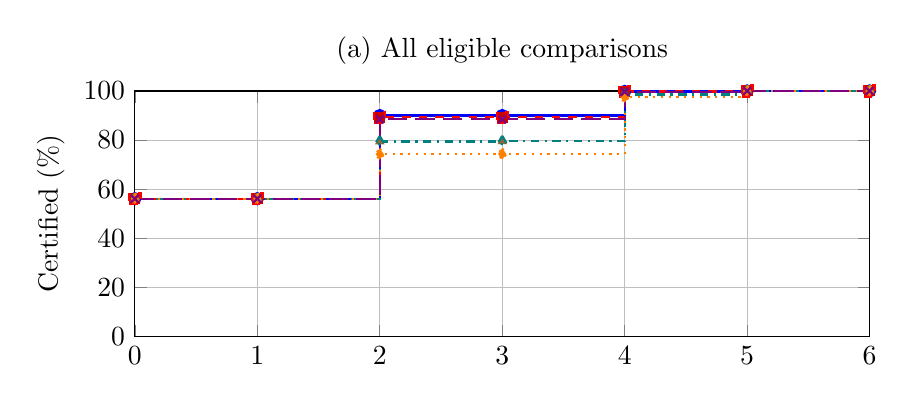
\begin{tikzpicture}
\begin{axis}[width=0.90\linewidth,height=4.7cm,xmin=0,xmax=6,ymin=0,ymax=100,
title={(a) All eligible comparisons},
xtick={0,1,2,3,4,5,6},ytick={0,20,40,60,80,100},
ylabel={Certified (\%)},grid=major,
xlabel={},]
\addplot+[const plot,thick,blue,solid,mark=*] coordinates {(0,56.123721) (1,56.123721) (2,89.976130) (3,89.987164) (4,99.799575) (5,100.000000) (6,100.000000)};
\addplot+[const plot,thick,red,dashed,mark=square*] coordinates {(0,56.123721) (1,56.123721) (2,89.244153) (3,89.261154) (4,99.811059) (5,100.000000) (6,100.000000)};
\addplot+[const plot,thick,teal,dashdotted,mark=triangle*] coordinates {(0,56.123721) (1,56.123721) (2,79.399308) (3,79.471028) (4,98.575273) (5,100.000000) (6,100.000000)};
\addplot+[const plot,thick,orange,dotted,mark=diamond*] coordinates {(0,56.123721) (1,56.123721) (2,74.234697) (3,74.334002) (4,97.512657) (5,100.000000) (6,100.000000)};
\addplot+[const plot,thick,violet,dash pattern=on 7pt off 3pt,mark=x] coordinates {(0,56.123721) (1,56.123721) (2,88.422085) (3,88.433119) (4,99.641761) (5,100.000000) (6,100.000000)};
\end{axis}
\end{tikzpicture}
\par\medskip
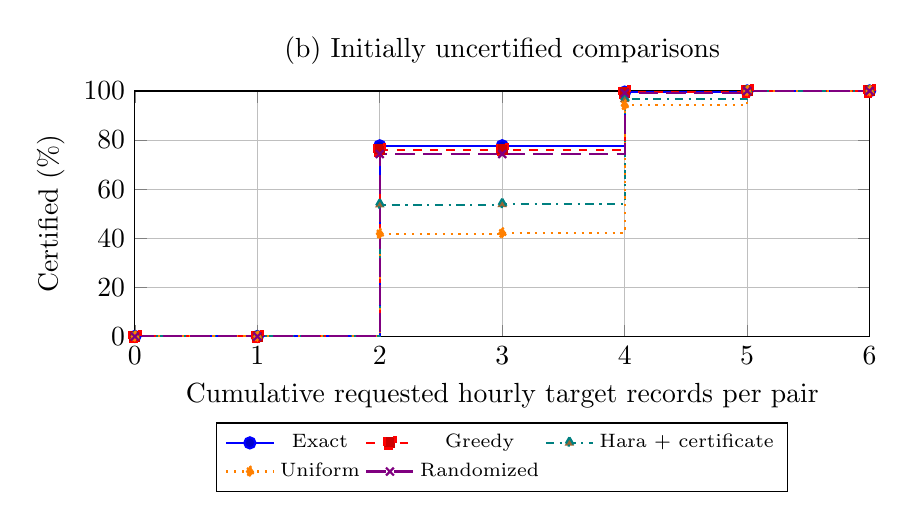
\begin{tikzpicture}
\begin{axis}[width=0.90\linewidth,height=4.7cm,xmin=0,xmax=6,ymin=0,ymax=100,
title={(b) Initially uncertified comparisons},
xtick={0,1,2,3,4,5,6},ytick={0,20,40,60,80,100},
ylabel={Certified (\%)},grid=major,
xlabel={Cumulative requested hourly target records per pair},
legend style={at={(0.5,-0.35)},anchor=north,legend columns=3,font=\scriptsize}]
\addplot+[const plot,thick,blue,solid,mark=*] coordinates {(0,0.000000) (1,0.000000) (2,77.645833) (3,77.673754) (4,99.528558) (5,100.000000) (6,100.000000)};
\addlegendentry{Exact}
\addplot+[const plot,thick,red,dashed,mark=square*] coordinates {(0,0.000000) (1,0.000000) (2,75.974582) (3,76.010792) (4,99.553249) (5,100.000000) (6,100.000000)};
\addlegendentry{Greedy}
\addplot+[const plot,thick,teal,dashdotted,mark=triangle*] coordinates {(0,0.000000) (1,0.000000) (2,53.663397) (3,53.844885) (4,96.602242) (5,100.000000) (6,100.000000)};
\addlegendentry{Hara + certificate}
\addplot+[const plot,thick,orange,dotted,mark=diamond*] coordinates {(0,0.000000) (1,0.000000) (2,41.841115) (3,42.088408) (4,94.123951) (5,100.000000) (6,100.000000)};
\addlegendentry{Uniform}
\addplot+[const plot,thick,violet,dash pattern=on 7pt off 3pt,mark=x] coordinates {(0,0.000000) (1,0.000000) (2,74.311930) (3,74.339851) (4,99.183512) (5,100.000000) (6,100.000000)};
\addlegendentry{Randomized}
\end{axis}
\end{tikzpicture}
\caption{External test decision curves under the early benchmark archive. Panel (a) retains every eligible comparison; panel (b) uses the common initially uncertified population. Each integer point uses executed batches and equal household weights within its panel. The staircase does not interpolate fractional requests. Randomized policies show the three fixed paths; they are not exact expectations over all possible acquisition trajectories.}
\label{fig:external-stopping}
\end{figure}
\begin{table}[htbp]
\centering\small\setlength{\tabcolsep}{4pt}
\caption{External early-archive acquisition costs and planning overhead. $U$ denotes initially uncertified cases and $A$ all eligible cases. Request means average households equally; the request median and planning mean/95th percentile pool cases in $U$. The stop/cap columns count all uncertified stops (including numerical ties) and unresolved cases at the six-request cap, respectively. All costs include failures. Planning covers acquisition selection, not forecast fitting or physical retrieval.}
\label{tab:external-costs}
\begin{tabular}{lrrrrr}
\toprule
Policy & Mean$_U$ & Median$_U$ & Mean$_A$ & Stop/cap & \shortstack{Planning\\mean/p95 (ms)}\\
\midrule
Exact & 2.452 & 2.0 & 1.080 & 0/0 & 0.82/1.65\\
Greedy & 2.485 & 2.0 & 1.094 & 0/0 & 0.81/1.66\\
Hara + certificate & 2.959 & 2.0 & 1.303 & 0/0 & 2.59/4.80\\
Uniform & 3.219 & 4.0 & 1.417 & 0/0 & 1.43/2.47\\
Randomized & 2.522 & 2.0 & 1.113 & 0/0 & 29.79/54.69\\
\bottomrule
\end{tabular}
\end{table}
\FloatBarrier
\subsection{Breadth, ties and reproducible checks}
Exact recovery has a strictly smaller attained $B_{80}$ than the better greedy/Hara baseline in 3 of 19 conditional household comparisons and 1 of 6 model pairs, including 0 learned-model pairs. A baseline that never attains 80\% is shown as NR, and is not assigned an invented numerical budget in these strict-improvement counts. Table~\ref{tab:external-pairs} preserves all pair-level outcomes; the supplement supplies every household and month.

\begin{table}[htbp]
\centering\small
\caption{External early-archive $B_{80}$ by model pair and among learned-model-only pairs. All rows use initially uncertified cases and equal household weights within that row. Pers. is two-day persistence; HGB is histogram gradient boosting.}
\label{tab:external-pairs}
\begin{tabular}{lrrrrr}
\toprule
Comparison & Exact & Greedy & Hara & Uniform & Randomized\\
\midrule
All pairs & 4 & 4 & 4 & 4 & 4\\
Learned pairs only & 4 & 4 & 4 & 4 & 4\\\midrule
Pers. vs HGB & 2 & 2 & 4 & 4 & 2\\
Pers. vs MLP & 2 & 4 & 4 & 4 & 4\\
Pers. vs Ridge & 2 & 2 & 4 & 4 & 4\\
HGB vs MLP & 4 & 4 & 4 & 4 & 4\\
Ridge vs HGB & 4 & 4 & 4 & 4 & 4\\
Ridge vs MLP & 4 & 4 & 4 & 4 & 4\\
\bottomrule
\end{tabular}
\end{table}

At its final stopping state, exact recovery has 0 unresolved cases and 0 numerical-tie stops in the initially uncertified population. Numerical ties are not counted as strict decisions. The corresponding exact and near-zero reference-contrast counts are 0 and 0, respectively; the near-zero count includes exact ties.

The validation replay is a calibration diagnostic because the Hara surrogate uses the full validation-period residual scale. Its $B_{80}$ values, in the same policy order, are 4, 4, 4, 4, 4. The test comparison freezes that scale and the acquisition code before test evaluation; validation is not presented as a second prospective cohort.

A separately written checker reconstructs the source features, archive copies, aggregate deductions, paid-query accounting, every saved acquisition stage and household-macro tables. It checks 52,995 test batches and 76,723 validation batches. Both runs have zero detected incorrect certificates, enclosure failures, timestamp violations, duplicate paid requests and cap violations. This is an independent implementation within the study, not external-investigator replication; it does not independently refit the models or prove each acquisition routine optimal. A logged observation-snapshot alias was repaired without changing query choices or outcomes; original and corrected traces are independently compared in the supplement.



\section{Additional Designs, Extensions, and Energy Results}\label{app:additional}
This appendix retains the supporting designs and complete analyses. The
original uniform-random retrieval baseline in its tables is distinct from
the optimized batch distribution of Section~\ref{sec:randomized-recovery}.
\subsection{Daily decisions and the value of pairing}\label{app:restricted-daily}
For two missing hours and exact six-hour totals, paired resolution was
71.5\%, 91.8\%, 91.8\% for Portugal, the household,
and the counter cohort, respectively; separate individual-error bounds
resolved 21.9\%, 62.7\%, 61.6\%. At six missing
hours the corresponding paired rates were 18.8\%, 48.9\%, 43.9\%,
versus 1.9\%, 8.6\%, 8.6\% for separate bounds.
The Portugal six-hour-gap gain was 16.9
percentage points (descriptive whole-meter bootstrap 95\% interval:
13.7--20.1).
Both methods receive identical measurements. Their difference therefore
isolates the benefit of comparing against the shared unknown target.

The profile imputer made daily ordering errors of
4.6\%, 3.5\%, 4.5\% in that setting, while deciding
100.0\%, 100.0\%, 100.0\% of comparisons.
Certified decisions trade coverage for a conditional all-completions
guarantee; these figures alone do not establish error-rate superiority
at equal coverage. With twelve missing hours and only a daily total,
paired resolution fell to 2.8\%, 3.7\%, 4.7\%.
The complete contiguous-gap grid is retained in Table~\ref{tab:daily}.
\begin{table*}[htbp]
\centering\normalsize\setlength{\tabcolsep}{4pt}
\caption{Frozen restricted-record daily evaluation; no saved-archive reconstruction. Daily comparison results for contiguous gaps and exact totals. Gap and total are hours. Paired and Separate columns give resolved comparisons (\%); the four point-method columns give errors among decisions (\%). Both bounding methods made zero incorrect decisions. Point methods make nearly all decisions; their higher coverage must be considered when comparing errors. Rates are macro-averaged over meters. Unresolved fraction is 100 minus resolved percentage.}
\label{tab:daily}
\begin{tabular}{lrrrrrrrr}
\toprule
Source & Gap & Total & Paired & Separate & Deletion & Uniform & Profile & Donor\\
\midrule
Portugal & 2 & 6 & 71.5 & 21.9 & 4.1 & 1.3 & 0.9 & 0.9\\
Portugal & 2 & 24 & 66.4 & 8.9 & 4.1 & 1.6 & 1.1 & 1.1\\
Portugal & 6 & 6 & 18.8 & 1.9 & 10.3 & 7.5 & 4.6 & 5.0\\
Portugal & 6 & 24 & 13.5 & 1.3 & 10.3 & 10.5 & 6.2 & 6.4\\
Portugal & 12 & 6 & 5.8 & 0.6 & 20.2 & 13.5 & 8.0 & 9.6\\
Portugal & 12 & 24 & 2.8 & 0.3 & 20.2 & 21.0 & 13.0 & 13.9\\
Household & 2 & 6 & 91.8 & 62.7 & 4.5 & 0.9 & 0.8 & 1.1\\
Household & 2 & 24 & 90.3 & 56.2 & 4.5 & 1.2 & 1.0 & 1.3\\
Household & 6 & 6 & 48.9 & 8.6 & 10.7 & 4.6 & 3.5 & 5.5\\
Household & 6 & 24 & 34.8 & 4.9 & 10.7 & 7.5 & 5.4 & 7.2\\
Household & 12 & 6 & 13.0 & 0.4 & 20.0 & 8.6 & 7.2 & 10.1\\
Household & 12 & 24 & 3.7 & 0.0 & 20.0 & 15.3 & 13.0 & 16.6\\
Counters & 2 & 6 & 91.8 & 61.6 & 4.0 & 1.0 & 0.7 & 0.8\\
Counters & 2 & 24 & 89.7 & 53.5 & 4.0 & 1.1 & 0.9 & 1.1\\
Counters & 6 & 6 & 43.9 & 8.6 & 11.8 & 5.6 & 4.5 & 5.3\\
Counters & 6 & 24 & 30.6 & 4.9 & 11.8 & 7.4 & 5.7 & 6.8\\
Counters & 12 & 6 & 11.6 & 1.7 & 24.3 & 11.2 & 8.7 & 11.4\\
Counters & 12 & 24 & 4.7 & 0.3 & 24.3 & 17.4 & 12.7 & 16.3\\
\bottomrule
\end{tabular}
\end{table*}

\FloatBarrier

\subsection{Budgeted recovery of measured values}\label{app:restricted-recovery}
Table~\ref{tab:recovery} reports the complete recovery grid. For six-hour
gaps, allowing two selected readings per pair raised paired resolution
from 18.8\%, 48.9\%, and 43.9\% to
60.1\%, 89.2\%, and 86.9\% for Portugal,
the household, and the counter cohort, respectively. The recovered values
are actual withheld readings; no synthetic completion is substituted for
them. All newly certified decisions remained correct.

The optimal rule left 28.6\%, 25.7\%, and 23.5\% of
the initial worst-case width at that budget, compared with
31.0\%, 28.1\%, and 25.3\% for greedy width
reduction. The implementation checked on every comparison that the
optimal batch's worst-case width was no larger than each baseline's and
that the realized post-recovery width was within its predicted bound.
These are the optimized criterion and its direct numerical verification.
Table~\ref{tab:width} reports the width comparison across gap sizes;
Appendix~\ref{app:neural-pairs} also displays coverage and worst-case width across budgets.
\begin{table*}[htbp]
\centering\normalsize\setlength{\tabcolsep}{4pt}
\caption{Frozen restricted-record daily evaluation; no saved-archive reconstruction. Completed recovery experiment: exact six-hour totals, three mask seeds, pair-specific batch queries. All six policy columns are final resolution (\%), macro-averaged over meters. Wt.: weighted sampling without replacement, using prediction-only contrast weights inspired by active comparison. Every certificate was correct. Optimal refers to worst-case width, not a guarantee of maximum empirical resolution. All policies use at most the listed number of recovered targets.}
\label{tab:recovery}
\begin{tabular}{lrrrrrrrr}
\toprule
Source & Gap & Budget & Optimal & Greedy & Uniform random & Max. $|c|$ & Wt. $|c|$ & Wt. $c^2$\\
\midrule
Portugal & 6 & 0 & 18.8 & 18.8 & 18.8 & 18.8 & 18.8 & 18.8\\
Portugal & 6 & 1 & 35.1 & 35.1 & 25.3 & 30.5 & 26.4 & 27.7\\
Portugal & 6 & 2 & 60.1 & 58.9 & 36.8 & 48.0 & 40.3 & 43.1\\
Portugal & 6 & 3 & 86.1 & 85.2 & 57.0 & 71.9 & 63.4 & 67.3\\
Portugal & 12 & 0 & 5.8 & 5.8 & 5.8 & 5.8 & 5.8 & 5.8\\
Portugal & 12 & 1 & 9.2 & 9.2 & 6.7 & 8.0 & 6.9 & 7.2\\
Portugal & 12 & 2 & 14.2 & 13.8 & 8.1 & 10.9 & 8.6 & 9.4\\
Portugal & 12 & 3 & 21.6 & 20.3 & 9.8 & 14.9 & 11.1 & 12.4\\
Household & 6 & 0 & 48.9 & 48.9 & 48.9 & 48.9 & 48.9 & 48.9\\
Household & 6 & 1 & 73.0 & 73.0 & 58.8 & 66.7 & 61.3 & 63.3\\
Household & 6 & 2 & 89.2 & 88.3 & 71.1 & 81.7 & 75.8 & 78.2\\
Household & 6 & 3 & 97.1 & 96.6 & 84.7 & 93.1 & 88.7 & 90.3\\
Household & 12 & 0 & 13.0 & 13.0 & 13.0 & 13.0 & 13.0 & 13.0\\
Household & 12 & 1 & 28.3 & 28.3 & 16.6 & 23.0 & 18.2 & 19.8\\
Household & 12 & 2 & 44.6 & 43.5 & 21.8 & 34.0 & 25.2 & 28.3\\
Household & 12 & 3 & 60.8 & 58.5 & 28.1 & 46.7 & 33.5 & 38.7\\
Counters & 6 & 0 & 43.9 & 43.9 & 43.9 & 43.9 & 43.9 & 43.9\\
Counters & 6 & 1 & 70.2 & 70.2 & 55.7 & 65.2 & 58.5 & 61.5\\
Counters & 6 & 2 & 86.9 & 86.2 & 67.3 & 80.5 & 73.8 & 77.5\\
Counters & 6 & 3 & 96.7 & 96.5 & 82.6 & 91.9 & 87.2 & 89.9\\
Counters & 12 & 0 & 11.6 & 11.6 & 11.6 & 11.6 & 11.6 & 11.6\\
Counters & 12 & 1 & 26.0 & 26.0 & 15.0 & 22.1 & 16.8 & 19.5\\
Counters & 12 & 2 & 40.8 & 39.4 & 19.8 & 32.4 & 23.9 & 27.2\\
Counters & 12 & 3 & 56.2 & 53.2 & 25.2 & 43.9 & 31.9 & 36.7\\
\bottomrule
\end{tabular}
\end{table*}
\begin{table*}[htbp]
\centering\normalsize\setlength{\tabcolsep}{4pt}
\caption{Frozen restricted-record daily evaluation; no saved-archive reconstruction. Remaining worst-case width (\% of initial width) with budget two. Within each meter, total remaining width is divided by total initial width; ratios are then macro-averaged. This is the objective optimized by the proposed recovery rule.}
\label{tab:width}
\begin{tabular}{lrrrrrrr}
\toprule
Source & Gap & Optimal & Greedy & Uniform random & Max. $|c|$ & Wt. $|c|$ & Wt. $c^2$\\
\midrule
Portugal & 6 & 28.6 & 31.0 & 72.7 & 46.8 & 63.1 & 57.2\\
Portugal & 12 & 52.8 & 54.9 & 89.5 & 69.4 & 84.4 & 79.6\\
Household & 6 & 25.7 & 28.1 & 71.4 & 44.5 & 60.8 & 53.7\\
Household & 12 & 50.8 & 52.7 & 90.0 & 67.9 & 83.9 & 78.6\\
Counters & 6 & 23.5 & 25.3 & 69.2 & 38.2 & 53.9 & 46.5\\
Counters & 12 & 46.2 & 48.0 & 88.6 & 58.8 & 77.9 & 69.8\\
\bottomrule
\end{tabular}
\end{table*}

At the same two-query budget, random recovery resolved
36.8\%, 71.1\%, and 67.3\%, while greedy
width reduction resolved 58.9\%, 88.3\%, and 86.2\%.
The gains over no recovery and the differences between recovery policies
answer distinct questions. The former measures the value of additional
readings; the latter measures how efficiently the budget is allocated.
The optimized quantity is worst-case width, while empirical resolution
also depends on the location of the interval relative to zero.

The optimal-width policy had at least as high aggregate resolution as
each comparator in these cohort/gap/budget settings. This empirical
observation is limited to the evaluated records; the theorem guarantees
worst-case width optimality, not resolution optimality at an arbitrary
realized completion.

\subsection{Recovery with independently bounded totals}\label{app:interval-theory}\label{sec:interval-recovery}
The exact-total model can be extended without imposing a load-shape model.
After subtracting observed values, let each independent block satisfy
$0\leq L_g\leq\sum_{i\in\M_g}y_i\leq U_g<\infty$.
Query answers remain exact, targets are nonnegative and uncapped, and
each query has unit cost. For a nonempty retained set with coefficient
extremes $\alpha\leq\beta$, define
\begin{equation}
 F_{L,U}(\alpha,\beta)=
 U\max(\beta,0)+L\min(\beta,0)
 -L\max(\alpha,0)-U\min(\alpha,0).
 \label{eq:interval-recovery-cost}
\end{equation}
\begin{proposition}[Batch recovery under total intervals]
For a fixed batch leaving at least one unknown coordinate in a block,
its worst-case remaining comparison width is
$F_{L_g,U_g}(\alpha,\beta)$. For each local query count, an optimal
retained set is a consecutive window in sorted coefficient order.
The allocation recurrence therefore remains exact when its local costs
use \eqref{eq:interval-recovery-cost} and allow full-block recovery at
zero remaining width.
\end{proposition}
\begin{proof}
If the queried values sum to $S$, the residual total interval is
$[\ell,u]=[\max(0,L-S),U-S]$. The queried contribution shifts both
comparison endpoints equally. The remaining width is $u\beta-\ell\alpha$
when $\alpha\geq0$, $\ell\beta-u\alpha$ when $\beta\leq0$, and
$u(\beta-\alpha)$ when $\alpha\leq0\leq\beta$. Each expression is
nonincreasing in feasible $S$: below $L$ its slope is
$\alpha-\beta$; above $L$ the respective slopes are $-\beta$,
$\alpha$, and $\alpha-\beta$. Zero queried values are feasible whenever
a coordinate remains, by assigning the required total to that remainder.
Hence the worst width occurs at $S=0$, yielding
\eqref{eq:interval-recovery-cost}. This cost is nondecreasing in
$\beta$ and nonincreasing in $\alpha$. Any retained subset can be
replaced by a consecutive window of the same size with extremes inside
its extremes, without increasing cost. Independent blocks contribute
additively, so the budget-allocation recurrence applies. A fully queried
block has no unknown contribution and contributes zero width.
\end{proof}
Two implementation details distinguish this extension from exact totals.
A singleton with coefficient $c$ retains width $(U-L)|c|$; querying it
may therefore be necessary. Likewise, constant coefficients need not
imply zero width. Local budgets must include $k_g=m_g$, and a block
can be skipped only when its actual width is zero. The released
\texttt{interval\_total\_recovery.py} implements these rules separately
from the primary exact-total experimental code. The result does not
assume independent stochastic errors; it assumes a product of declared
total intervals. Additional known correlations require a different set.
Uncertain query answers, overlapping constraints, target capacity limits
and unequal costs remain outside this implementation.


% Integration fragment: uses the main manuscript's proposition/proof environments.
% Place after deterministic adaptive recovery; replace its short randomized example.
% Requires bibliography keys kawase2024 and mastin2015 (see bibitem_suggestions.tex).

\subsection{Daily fairness and close-competitor diagnostics}\label{app:fairness-design}
In response to methodological review, we add exploratory daily analyses for
the six-hour contiguous gap, exact six-hour totals, and all three fixed
mask seeds. These analyses reuse every eligible saved forecast without
refitting. At budgets zero and two, each point evaluator receives exactly
the same recovered observations as the sharp comparison for that model pair.
At budget two, these are the optimal width-minimizing batch and its actual
withheld values; donor matching and residual-energy allocation are then
updated using the expanded visible record.

Within each cohort, budget, and named pair (and separately across all pairs),
selective point evaluators rank the absolute estimated comparison margin
divided by the squared training mean. Stable meter/day/seed/pair ordering
breaks ties. The selected count is matched to the sharp method's number
of certificates; additional curves retain 5\% through 100\% of comparisons.
Selection uses visible scores, not complete-reference errors. The error
rate is the pooled number of wrong decisions divided by selected decisions.
Each meter in a cohort contributes the same number of days, so pooled
certificate coverage also equals its meter macro-average. These descriptive
rates are not independent-trial estimates.

Named-pair results address comparisons among the learned models directly.
For interpretation only, we also divide comparisons into five equal-count
strata ordered by the absolute complete-reference daily MSE difference,
normalized by the squared training mean. Strata are fixed at budget zero
and reused at budget two; deterministic ordering can place tied margins
in adjacent rank quintiles. Their hidden-reference margin is never used for
query selection or abstention; this post-hoc diagnostic measures difficulty,
not a deployable selection rule.



\subsection{Evaluator-access sensitivity}\label{app:access-design}
The primary restricted-record experiment conditions on the current day's
predictions, surviving targets and retained totals. A post-review protocol
adds a second regime: all available saved test persistence predictions
for that meter. The implemented persistence forecast at $t+24$ hours is
an exact copy of the actual measurement at $t$. A timestamp lookup built
from forecast columns alone therefore reveals a masked target whenever
that later forecast is present. Its provenance is checked against the
fixed feature-construction code; equality with hidden truth is checked
only afterward. No lookup falls back to raw measurements.

We first add these free values to the observed set, then recompute sharp
bounds and batches of at most two paid queries. The same six- and
twelve-hour gaps, six-hour totals, three seeds, six model pairs and all
34 meters are retained. Paid batches never request an already revealed
value. Restricted-regime counts and widths are reconciled with the original
recovery archive. Both exact and greedy policies retain the original
all-case budget convention, including already certified pairs; average
queries do not estimate an optimal early-stopping policy.

This is retrospective access to the available saved test persistence
archive, including future records. It is not a same-day access model,
full informational closure, or a new blind validation cohort. Missing
future archive rows remain unavailable; nonlinear inversion, feature
caches and records outside this archive are excluded. If persistence
used imputed inputs, its output would not establish a measured target.
Free-recovery fractions count masked coordinate occurrences; repeated
seeds and model pairs do not constitute independent observations.



\subsection{Frozen replication on previously unused consumers}\label{app:replication-design}
After the original analyses, a dated local protocol fixed a replication
before evaluating additional consumers from the same UCI Portugal source.
The documented original loaders accessed only meter IDs MT\_001--MT\_080.
Candidates were MT\_081--MT\_370 in ascending order; the first 30 meeting
the original 2013-only coverage and positivity rule were selected.
All selected IDs are disjoint from the original panel. The supplement
records every candidate's training eligibility, the selected IDs, source
and code hashes, and the protocol. Selection does not depend on 2014
forecast errors, recovery results or convergence warnings.

The original timestamp conversion, causal features, daylight-saving
exclusions, 2013 training year, 2014 test windows, four model specifications
and training allowance were frozen. Each new consumer received a separate
fit using its own training history. This evaluates a fixed procedure on
previously unused consumers, not zero-shot transfer or a new data source.
No retuning, fit retry or outcome-driven consumer replacement was allowed.
The primary endpoint uses six-hour contiguous gaps, exact six-hour totals,
the three original mask seeds, all six model pairs and budgets zero and
at most two. Exact and greedy recovery are evaluated under both declared
access regimes. Primary rates weight consumers equally; pooled counts and
rates are supplied separately. Descriptive paired percentile intervals
use 2,000 whole-consumer bootstrap resamples with seed 1729. The consumers
share a historical source and test calendar, so these intervals do not
establish independent-population generalization. This local protocol is
not an independently registered study.



\subsection{Interval-total recovery sensitivity on frozen traces}\label{app:interval-design}
A separate protocol, fixed before its outcomes, evaluates the interval-total
batch solver on the original 34 series and all 3,729 held-out meter-days.
No forecasting model is refitted. The six-hour contiguous gaps, six-hour
blocks, three original mask seeds and all six model pairs are retained.
For each complete reference block total $T$, the supplied interval is
$[(1-\tau)T,(1+\tau)T]$, with $\tau\in\{0,0.01,0.05\}$.
These are constructed sensitivity bands, not calibrated instrument errors
or independent backup measurements.

Both daily access regimes include all exact deductions from retained
totals: an exact singleton residual and every zero-upper-residual block
are revealed without a query. An interval-valued singleton remains unknown.
The saved-archive regime additionally uses every documented persistence
copy in the available test forecasts before making these deductions.
The restricted regime supplies only the isolated daily record and its totals.
The exact batch globally minimizes the worst-width objective. The greedy
batch successively chooses the largest one-step reduction in that same
objective; ties use the smallest target index. A batch receives at
most two exact target answers \emph{per day and model pair}; no answer is
visible during selection, and full-block recovery is permitted.
Freely known or determined values cannot consume the budget.
This eligibility check uses the information available before batch selection.
The experiment does not cancel or refund a later batch request when an
earlier returned answer would make it inferable; it is not an adaptive
early-stopping cost study.
All cases, including already certified comparisons, are retained.
Rates and width summaries average within meters and then equally across
meters in each cohort. Raw widths and widths normalized by squared training
mean energy are supplied alongside paid-query and deduction counts.




\subsection{Daily decisions at equal coverage}\label{app:matched-daily}
Table~\ref{tab:dailymatched} supplies the daily matched-coverage comparison,
including equal-information evaluation after recovery. Figure~\ref{fig:dailycoverage}
shows how selective point-method errors change with coverage. Neither
analysis tunes a threshold against hidden outcomes. Zero certificate errors
are expected when the reference is feasible and the implementation is
correct; the coverage and query requirements determine the empirical usefulness.
\begin{table*}[htbp]
\centering\normalsize\setlength{\tabcolsep}{4pt}
\caption{Frozen restricted-record daily evaluation; no saved-archive reconstruction. Daily errors (\%) among selected comparisons at identical coverage (\%). All six named pairs and three seeds; six-hour gaps and totals. The sharp method has zero observed error in every row. Budget two supplies the same pair-specific recovered readings to all evaluators. Selective errors are pooled wrong/selected counts; coverage equals the cohort\textquotesingle s meter macro-average.}
\label{tab:dailymatched}
\begin{tabular}{lrrrrrr}
\toprule
Source & Budget & Coverage & Deletion & Uniform & Profile & Donor\\
\midrule
Portugal & 0 & 18.8 & 1.345 & 0.939 & 0.276 & 0.193\\
Portugal & 2 & 60.1 & 1.406 & 0.135 & 0.035 & 0.049\\
Household & 0 & 48.9 & 1.847 & 0.323 & 0.231 & 0.970\\
Household & 2 & 89.2 & 3.923 & 0.228 & 0.152 & 0.177\\
Counters & 0 & 43.9 & 3.712 & 1.160 & 0.325 & 0.742\\
Counters & 2 & 86.9 & 4.030 & 0.164 & 0.070 & 0.187\\
\bottomrule
\end{tabular}
\end{table*}
For Portugal at budget two, profile and donor imputation make
12 and 17 wrong decisions,
respectively, among 34,718 selected comparisons each.
The sharp method certifies the same number without an incorrect decision.
The point-method errors are small; these observed differences concern this
specified selective rule and panel, rather than all possible imputation
methods or future records.
\begin{figure}[htbp]\centering
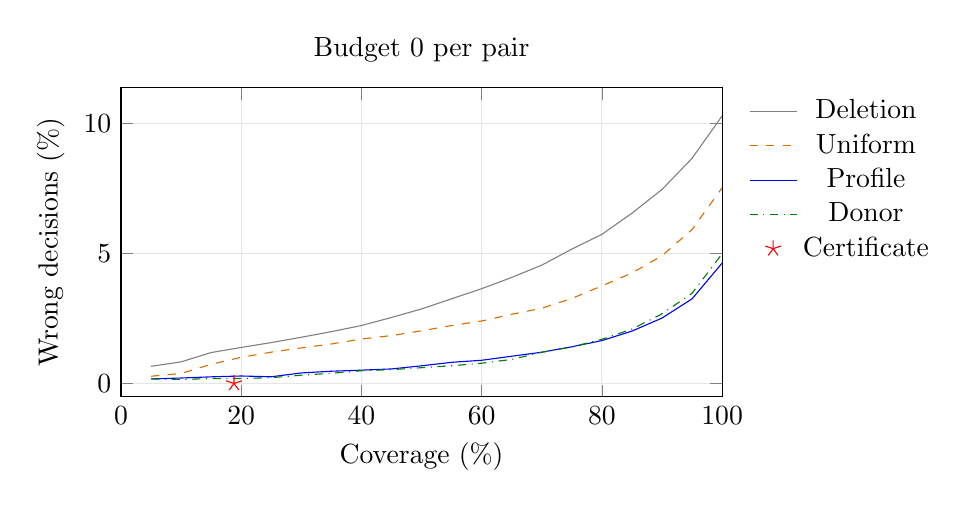
\begin{tikzpicture}
\begin{axis}[width=0.76\linewidth,height=5.5cm,tick label style={font=\normalsize},label style={font=\normalsize},legend style={font=\normalsize,draw=none},grid=major,grid style={gray!20},scaled ticks=false,xmin=0,xmax=100,ymin=-0.5,xlabel={Coverage (\%)},ylabel={Wrong decisions (\%)},legend pos=outer north east,title={Budget 0 per pair}]
\addplot+[gray,mark=none] coordinates {(5,0.6576670128) (10,0.8307372793) (15,1.18841583) (20,1.384562132) (25,1.57147802) (30,1.776854736) (35,1.992780497) (40,2.228279682) (45,2.538363909) (50,2.866043614) (55,3.256867743) (60,3.646013615) (65,4.079133051) (70,4.55174801) (75,5.16903196) (80,5.737279335) (85,6.550200558) (90,7.463174493) (95,8.662622288) (100,10.29421945)};
\addlegendentry{Deletion}
\addplot+[orange!85!black,mark=none,dashed] coordinates {(5,0.2769124264) (10,0.3807545864) (15,0.7384331372) (20,1.003807546) (25,1.204569055) (30,1.367255106) (35,1.518073481) (40,1.709068882) (45,1.842236837) (50,2.024922118) (55,2.22788634) (60,2.4027922) (65,2.659956866) (70,2.892745883) (75,3.269874236) (80,3.753461405) (85,4.249384073) (90,4.915195569) (95,5.920824908) (100,7.526825891)};
\addlegendentry{Uniform}
\addplot+[blue,mark=none] coordinates {(5,0.1730702665) (10,0.2076843198) (15,0.2538363909) (20,0.2855659398) (25,0.2561439945) (30,0.4038306219) (35,0.469762152) (40,0.5105572863) (45,0.5576708588) (50,0.6784354448) (55,0.8118568866) (60,0.8913118726) (65,1.046409458) (70,1.201602136) (75,1.409945771) (80,1.648494289) (85,2.013723454) (90,2.515287874) (95,3.255542803) (100,4.62962963)};
\addlegendentry{Profile}
\addplot+[green!50!black,mark=none,dashdotted] coordinates {(5,0.1730702665) (10,0.1557632399) (15,0.1846082843) (20,0.1903772932) (25,0.2215299412) (30,0.3172954886) (35,0.3906443159) (40,0.4889235029) (45,0.5307488174) (50,0.6057459328) (55,0.6796941376) (60,0.7788161994) (65,0.9239289613) (70,1.199129704) (75,1.403022961) (80,1.69825199) (85,2.091096044) (90,2.676820122) (95,3.470514292) (100,4.986154379)};
\addlegendentry{Donor}
\addplot+[red,only marks,mark=star,mark size=3pt] coordinates {(18.79196954,0)};
\addlegendentry{Certificate}
\end{axis}
\end{tikzpicture}

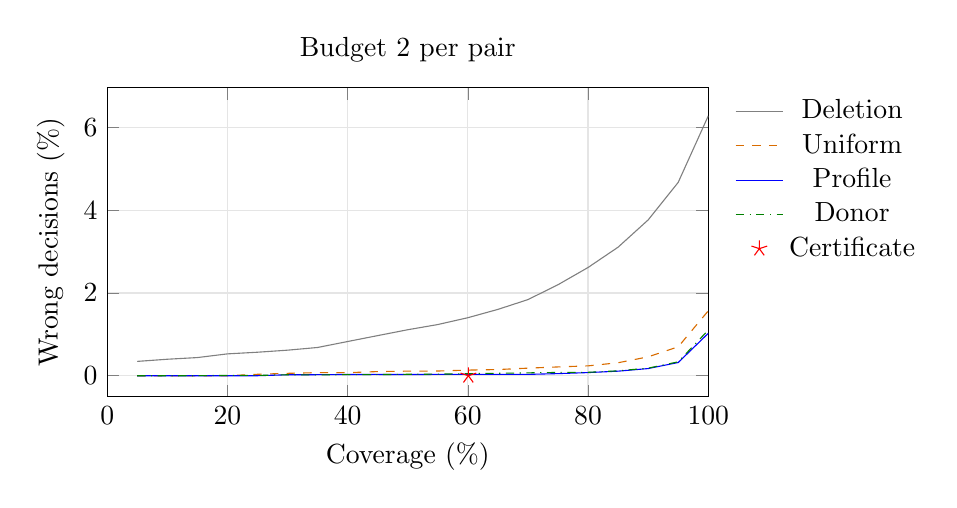
\begin{tikzpicture}
\begin{axis}[width=0.76\linewidth,height=5.5cm,tick label style={font=\normalsize},label style={font=\normalsize},legend style={font=\normalsize,draw=none},grid=major,grid style={gray!20},scaled ticks=false,xmin=0,xmax=100,ymin=-0.5,xlabel={Coverage (\%)},ylabel={Wrong decisions (\%)},legend pos=outer north east,title={Budget 2 per pair}]
\addplot+[gray,mark=none] coordinates {(5,0.3461405331) (10,0.398061613) (15,0.4384446752) (20,0.5278643129) (25,0.5676704742) (30,0.6172839506) (35,0.6823913366) (40,0.8264105227) (45,0.9691934926) (50,1.111111111) (55,1.236665723) (60,1.401869159) (65,1.60289693) (70,1.83948969) (75,2.199146187) (80,2.615524403) (85,3.107120314) (90,3.765239798) (95,4.672897196) (100,6.27898927)};
\addlegendentry{Deletion}
\addplot+[orange!85!black,mark=none,dashed] coordinates {(5,0) (10,0) (15,0) (20,0) (25,0.03461405331) (30,0.05769008884) (35,0.07417297137) (40,0.07355486327) (45,0.09999615399) (50,0.1107649706) (55,0.1132823563) (60,0.1355717088) (65,0.1491066912) (70,0.182959996) (75,0.2122995269) (80,0.2379716165) (85,0.3135626005) (90,0.4557517019) (95,0.697746443) (100,1.568016615)};
\addlegendentry{Uniform}
\addplot+[blue,mark=none] coordinates {(5,0) (10,0) (15,0) (20,0) (25,0) (30,0.02307603554) (35,0.02472432379) (40,0.03028729664) (45,0.03076804738) (50,0.02769124264) (55,0.03146732119) (60,0.03461405331) (65,0.03195143382) (70,0.03214162093) (75,0.05076727818) (80,0.07571824161) (85,0.1099505223) (90,0.1730702665) (95,0.3188136489) (100,1.024575978)};
\addlegendentry{Profile}
\addplot+[green!50!black,mark=none,dashdotted] coordinates {(5,0) (10,0) (15,0) (20,0.008653513326) (25,0.006922810661) (30,0.02307603554) (35,0.01977945903) (40,0.02596053998) (45,0.02692204146) (50,0.03461405331) (55,0.03776078542) (60,0.04903657552) (65,0.05857762867) (70,0.06922810661) (75,0.07845852083) (80,0.0822083766) (85,0.1180950054) (90,0.1826852813) (95,0.3352097794) (100,1.100726895)};
\addlegendentry{Donor}
\addplot+[red,only marks,mark=star,mark size=3pt] coordinates {(60.08653513,0)};
\addlegendentry{Certificate}
\end{axis}
\end{tikzpicture}

\caption{Frozen restricted-record daily evaluation; no saved-archive reconstruction. Daily error versus coverage in the Portugal panel, six-hour gaps and exact six-hour totals. Every evaluator receives the same optimal-batch recovered values at budget two. Curves select by visible estimated margins; the star shows the sharp method\textquotesingle s attained coverage and observed error. Complete-reference losses are used only after selection to count errors. All values are descriptive on this fixed panel.}
\label{fig:dailycoverage}\end{figure}
\FloatBarrier

\subsection{Named competitors and comparison difficulty}\label{app:named-pairs}
Table~\ref{tab:namedpairs} separates every model pair in the primary panel,
including ridge versus boosting and ridge versus MLP. These comparisons
prevent aggregate coverage from being attributed solely to the difference
between persistence and learned forecasts. The complete-reference margin
strata in Table~\ref{tab:marginstrata} further isolate close daily comparisons;
they are explanatory strata formed after evaluation, not information
available to the audit.
\begin{table}[htbp]
\centering\normalsize\setlength{\tabcolsep}{4pt}
\caption{Frozen restricted-record daily evaluation; no saved-archive reconstruction. Certified daily comparisons (\%) by named model pair, six-hour gaps and exact six-hour totals. The full cohort and pair breakdown is in \texttt{study\_daily\_pairs.csv}.}
\label{tab:namedpairs}
\begin{tabular}{lrr}
\toprule
Portugal model pair & Before & Budget two\\
\midrule
Daily--Boosting & 24.9 & 66.2\\
Daily--MLP & 21.5 & 61.7\\
Daily--Ridge & 25.5 & 67.1\\
Boosting--MLP & 10.7 & 51.3\\
Ridge--Boosting & 16.5 & 59.4\\
Ridge--MLP & 13.7 & 54.8\\
\bottomrule
\end{tabular}
\end{table}
\begin{table}[htbp]
\centering\normalsize\setlength{\tabcolsep}{4pt}
\caption{Frozen restricted-record daily evaluation; no saved-archive reconstruction. Portugal certification (\%) by increasing absolute normalized complete-reference daily loss margin, pooled over all six pairs. Quintile 1 contains the closest comparisons. The same cases define each stratum at both budgets; repeated mask seeds remain dependent. Pair-specific strata are archived in \texttt{study\_daily\_margin\_strata.csv}.}
\label{tab:marginstrata}
\begin{tabular}{lrrrr}
\toprule
Quintile & Min. margin & Max. margin & Before & Budget two\\
\midrule
1 & $2.853\times10^{-7}$ & 0.0014627 & 0.1 & 11.2\\
2 & 0.0014628 & 0.003581 & 1.0 & 40.2\\
3 & 0.0035814 & 0.0081389 & 6.3 & 66.0\\
4 & 0.0081464 & 0.021704 & 21.9 & 85.5\\
5 & 0.021704 & 4.0102 & 64.7 & 97.6\\
\bottomrule
\end{tabular}
\end{table}
In the closest-margin quintile, budget-two certification is
11.17\%, versus
97.56\% in the widest-margin quintile.
Recovery therefore helps close comparisons but does not remove their
identification difficulty. The named learned-model comparisons and the
small-margin strata should be considered together when assessing a use case.
\FloatBarrier


\subsection{Comparisons involving the neural forecaster}\label{app:neural-pairs}
Table~\ref{tab:neural} isolates MLP-versus-persistence, MLP-versus-ridge,
and MLP-versus-boosting comparisons, keeping every meter, test day, and
mask seed. This prevents the AI conclusion from resting only on an
aggregate that includes comparisons between simpler models. The audit
requires saved predictions and measurement constraints, so its procedure
is identical for the neural and other candidates. These results establish
its applicability to the trained MLP; they do not establish a new neural
architecture or state-of-the-art forecasting accuracy.
\begin{table*}[htbp]
\centering\normalsize\setlength{\tabcolsep}{4pt}
\caption{Frozen restricted-record daily evaluation; no saved-archive reconstruction. AI-specific audit: resolution (\%) for the three comparisons involving the neural MLP, six-hour gaps and exact six-hour totals. Before: no recovery. All other columns use budget two. This subset was specified before the revised results were calculated.}
\label{tab:neural}
\begin{tabular}{lrrrrrrr}
\toprule
Source & Before & Optimal & Greedy & Uniform random & Max. $|c|$ & Wt. $|c|$ & Wt. $c^2$\\
\midrule
Portugal & 15.3 & 55.9 & 54.8 & 32.5 & 43.0 & 35.4 & 38.0\\
Household & 44.4 & 87.8 & 86.5 & 68.2 & 78.5 & 72.5 & 75.4\\
Counters & 39.8 & 86.2 & 85.5 & 64.8 & 78.1 & 70.7 & 74.3\\
\bottomrule
\end{tabular}
\end{table*}
Figure~\ref{fig:recovery} displays coverage and worst-case width across budgets.
\begin{figure}[htbp]\centering
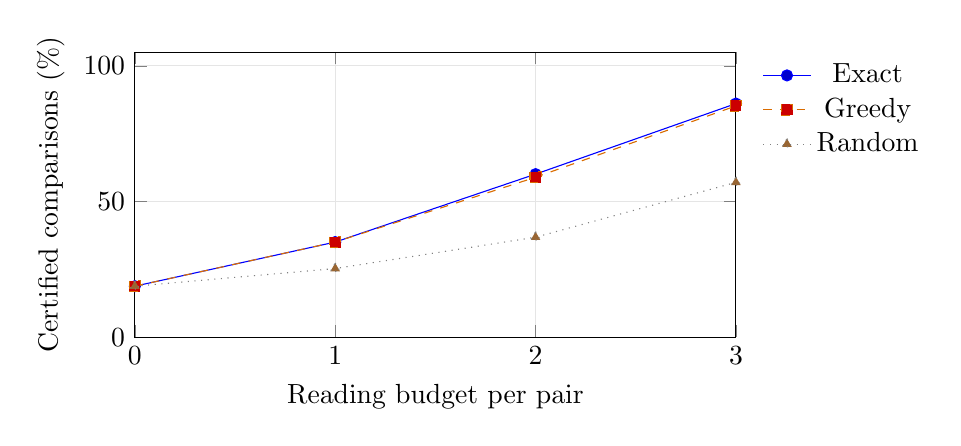
\begin{tikzpicture}
\begin{axis}[width=0.76\linewidth,height=5.2cm,tick label style={font=\normalsize},label style={font=\normalsize},legend style={font=\normalsize,draw=none},grid=major,grid style={gray!20},scaled ticks=false,xmin=0,xmax=3,xtick={0,1,2,3},ymin=0,ymax=105,xlabel={Reading budget per pair},ylabel={Certified comparisons (\%)},legend pos=outer north east]
\addplot+[blue,mark=*] coordinates {(0,18.79196954) (1,35.05019038) (2,60.08653513) (3,86.07995846)};
\addlegendentry{Exact}
\addplot+[orange!85!black,mark=square*,dashed] coordinates {(0,18.79196954) (1,35.05019038) (2,58.93388716) (3,85.22499135)};
\addlegendentry{Greedy}
\addplot+[gray,mark=triangle*,dotted] coordinates {(0,18.79196954) (1,25.29075805) (2,36.84146764) (3,57.04742125)};
\addlegendentry{Random}
\end{axis}
\end{tikzpicture}

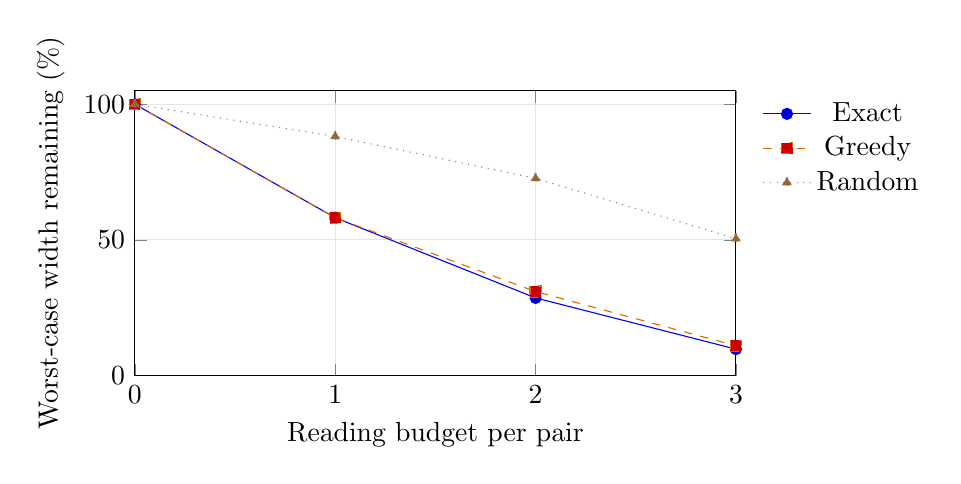
\begin{tikzpicture}
\begin{axis}[width=0.76\linewidth,height=5.2cm,tick label style={font=\normalsize},label style={font=\normalsize},legend style={font=\normalsize,draw=none},grid=major,grid style={gray!20},scaled ticks=false,xmin=0,xmax=3,xtick={0,1,2,3},ymin=0,ymax=105,xlabel={Reading budget per pair},ylabel={Worst-case width remaining (\%)},legend pos=outer north east]
\addplot+[blue,mark=*] coordinates {(0,100) (1,58.18690041) (2,28.62983522) (3,9.755222493)};
\addlegendentry{Exact}
\addplot+[orange!85!black,mark=square*,dashed] coordinates {(0,100) (1,58.18690041) (2,30.97520219) (3,11.00077593)};
\addlegendentry{Greedy}
\addplot+[gray,mark=triangle*,dotted] coordinates {(0,100) (1,88.13802378) (2,72.69957825) (3,50.45326371)};
\addlegendentry{Random}
\end{axis}
\end{tikzpicture}

\caption{Frozen restricted-record daily evaluation; no saved-archive reconstruction. Recovery in the Portugal panel: six missing hourly targets, exact six-hour totals, all six model pairs and three mask seeds. Curves are means of per-meter results. Top: realized certification coverage. Bottom: worst-case width relative to its no-recovery value, the criterion optimized. A width advantage need not give a coverage advantage at the observed truth.}
\label{fig:recovery}\end{figure}
\FloatBarrier

\subsection{Incremental benefit over greedy retrieval}\label{app:greedy-detail}
The gain over no recovery combines acquiring new data with selecting them.
To isolate allocation, we compare exact and greedy selection at the same
budget on every case. In Portugal at six missing hours and budget two,
the mean meter-level resolution difference is 1.15 percentage
points, with meter-level range 0.21 to 2.49.
The median is 1.19; across meter--seed summaries
the 10th and 90th percentiles are 0.47 and 1.87 points.
Exact selection alone resolves 785 dependent cases,
whereas greedy alone resolves 119. Thus the worst-case-width
optimum is not a pointwise optimum for realized certification.

Across these cases, the additional worst-case-width reduction of exact
over greedy, divided by initial width, has median 0.00\%, 90th percentile
3.41\%, and maximum 92.02\%.
Realized width is larger under the exact policy in 700 cases;
that outcome is compatible with optimizing a worst-case objective.
The complete signed distributions and pair/seed breakdowns are retained in
\texttt{recovery\_diagnostics.json}, \texttt{study\_recovery\_pair\_seed.csv},
and the full local \texttt{study\_recovery\_cases.csv}. The public package
supplies \texttt{study\_recovery\_cases\_public.csv} for UCI cases and
hashes plus regeneration instructions for the omitted BLEM case rows.
These post-review diagnostics include
all cases and are descriptive; repeated days, pairs, and seeds are dependent.
Table~\ref{tab:actualrecovery} complements the budget caps with actual query
counts and both realized and worst-case remaining widths.
\begin{table*}[htbp]
\centering\normalsize\setlength{\tabcolsep}{4pt}
\caption{Frozen restricted-record daily evaluation; no saved-archive reconstruction. Actual mean reading counts and remaining-width fractions (\%) at budget two, six-hour gaps and totals. Within-meter width fractions divide summed remaining width by summed initial width; cohort values macro-average meters. Queries are per specified pair, not the cost of ranking all four models. All policies and budgets appear in \texttt{study\_recovery.csv}.}
\label{tab:actualrecovery}
\begin{tabular}{llrrrr}
\toprule
Source & Policy & Queries & Actual width & Worst width & Resolved\\
\midrule
Portugal & Exact & 1.999 & 19.1 & 28.6 & 60.1\\
Portugal & Greedy & 1.999 & 20.5 & 31.0 & 58.9\\
Portugal & Uniform random & 1.999 & 47.8 & 72.7 & 36.8\\
Household & Exact & 2.000 & 17.2 & 25.7 & 89.2\\
Household & Greedy & 2.000 & 18.7 & 28.1 & 88.3\\
Household & Uniform random & 2.000 & 48.4 & 71.4 & 71.1\\
Counters & Exact & 2.000 & 15.6 & 23.5 & 86.9\\
Counters & Greedy & 2.000 & 16.7 & 25.3 & 86.2\\
Counters & Uniform random & 2.000 & 46.5 & 69.2 & 67.3\\
\bottomrule
\end{tabular}
\end{table*}
Table~\ref{tab:recoveryci} summarizes the paired meter-bootstrap
stability of the resolution gains, separately for all pairs and neural-model
pairs. Whole meters remain the resampling unit.
\begin{table}[htbp]
\centering\normalsize\setlength{\tabcolsep}{4pt}
\caption{Frozen restricted-record daily evaluation; no saved-archive reconstruction. Portugal resolution gain in percentage points: optimal recovery with budget two minus the reference policy, six-hour gaps and exact six-hour totals. Lower/Upper: descriptive 95\% paired bootstrap limits from 2,000 resamples of the same 30 whole meters. All days, pairs, and seeds remain aggregated within each meter. These are panel-stability intervals, not population-wide confidence claims.}
\label{tab:recoveryci}
\begin{tabular}{llrrr}
\toprule
Comparisons & Reference & Gain & Lower & Upper\\
\midrule
All pairs & No recovery & 41.29 & 38.85 & 43.52\\
All pairs & Greedy & 1.15 & 1.01 & 1.31\\
All pairs & Weighted $|c|$ & 19.83 & 18.58 & 20.87\\
All pairs & Weighted $c^2$ & 16.98 & 15.90 & 17.91\\
MLP pairs & No recovery & 40.64 & 38.67 & 42.69\\
MLP pairs & Greedy & 1.18 & 0.99 & 1.36\\
MLP pairs & Weighted $|c|$ & 20.56 & 19.40 & 21.56\\
MLP pairs & Weighted $c^2$ & 17.89 & 16.82 & 18.77\\
\bottomrule
\end{tabular}
\end{table}
\FloatBarrier

\subsection{Sensitivity to the available forecast archive}\label{app:earlier-access}\label{sec:archive-access}
Allowing the saved future persistence forecasts changes the information
problem substantially (Table~\ref{tab:archive-access}). The lookup reveals
most masked targets without paid recovery. These results are not additional
improvements attributable to the query optimizer: they arise from using
information already present in the broader archive.

\begin{table}[htbp]
\centering\small
\caption{Access to all available saved test persistence forecasts. Free:
percentage of originally masked target occurrences revealed before queries.
$C_0,C_2$: certified comparison percentages at zero and at most two paid
queries using the exact policy. $\Delta$: exact-minus-greedy $C_2$ in
percentage points. $\bar q$: actual mean paid queries per pair at budget two.
All figures include every case, not only previously unresolved comparisons.}
\label{tab:archive-access}
\begin{tabular}{lrrrrrr}
\toprule
Cohort & Gap (h) & Free (\%) & $C_0$ & $C_2$ & $\Delta$ & $\bar q$\\
\midrule
Portugal & 6 & 95.33 & 96.67 & 98.71 & +0.042 & 0.093\\
Portugal & 12 & 95.33 & 95.70 & 96.17 & +0.014 & 0.093\\
Household & 6 & 88.21 & 93.50 & 98.71 & +0.226 & 0.236\\
Household & 12 & 88.21 & 89.79 & 92.86 & +0.090 & 0.236\\
Counters & 6 & 98.90 & 99.45 & 99.82 & +0.020 & 0.022\\
Counters & 12 & 98.90 & 98.96 & 99.25 & +0.000 & 0.022\\
\bottomrule
\end{tabular}
\end{table}
The saved persistence copies match the reference targets exactly in the
stored binary64 data. Every recomputed comparison interval contains its
reference difference, and no certificate is incorrect. The restricted
regime reproduces 5,168
archived meter and named-pair/seed rows, including decision counts,
widths and mean queries. The sensitivity evaluates 1,073,952
dependent policy/budget/pair cases; this is a computation count, not an
independent statistical sample.

The large restricted-record gain from paid recovery therefore does not
carry over unchanged to an archive with these future exact copies.
The remaining uncertainty is concentrated at boundaries and gaps in the
available test archive. A practical audit should incorporate authorized
reconstructable targets first and allocate a recovery budget only to the
remaining unknowns. This analysis supports that workflow, but does not
measure field retrieval savings or establish how often a real evaluator
has only the restricted inputs.

\FloatBarrier

\subsection{Replication on 30 previously unused consumers}\label{app:replication-results}
\label{sec:newconsumers}
Table~\ref{tab:newconsumers} reports the replication. The fixed training-only rule selected 30 additional consumers from 255
eligible candidates. Each contributes 107 test days, giving 3,210
additional meter-days and 77,040 hourly targets.
The supplied targets and fixed forecasts range from 0.00 to
3,440.43 kWh per hourly target.
All 30 neural fits stopped in 28--383 epochs within the fixed allowance, with no captured training warnings. The analysis retains all 57,780
pair/mask comparisons per access regime. Policy and budget evaluations of
the same records are dependent; they are not additional independent samples.

\begin{table}[t]
\centering\small
\caption{Daily outcomes over three mask seeds. Frozen new-consumer replication: mean consumer-level certification
rates (\%) under six-hour gaps and totals. $q\leq2$ denotes an available
two-reading budget per model pair. Final column: mean readings actually
queried by exact recovery.}
\label{tab:newconsumers}
\begin{tabular}{lrrrr}
\toprule
Access & $q=0$ & Exact $q\leq2$ & Greedy $q\leq2$ & Queries\\
\midrule
Restricted record & 25.02 & 64.11 & 62.95 & 1.998\\
Saved archive & 96.87 & 98.57 & 98.51 & 0.093\\
\bottomrule
\end{tabular}
\end{table}

Restricted-record exact-minus-greedy coverage is 1.154 percentage points (descriptive 95\% consumer-bootstrap interval [1.004, 1.303]); 30 consumers favor exact recovery, 0 favor greedy and 0 tie.
Saved-archive exact-minus-greedy coverage is 0.061 percentage points (descriptive 95\% consumer-bootstrap interval [0.035, 0.088]); 18 consumers favor exact recovery, 2 favor greedy and 10 tie.
The saved archive reconstructs 95.327\% of masked targets without a query. No incorrect certificate,
truth-enclosure failure or violation of the predicted worst remaining
width occurred in the 462,240 dependent policy/budget
evaluations. Query eligibility and copied target values also passed the
recorded checks. Per-consumer, named-pair, seed and forecast-error tables,
along with these UCI-only predictions, are supplied for reconstruction.
This replication tests the fixed procedure beyond its development panel;
it does not supply production outage, target-arrival or retrieval-cost data.

A separate checker, importing none of the analysis implementations,
recomputes all 120 forecast-error rows and
115,560 zero-query comparisons,
and reconciles all pair/seed, consumer, cohort and named-pair aggregates.
Representative numerical checks additionally enumerate 2,882 direct-loss vertices
and 5,994 query subsets.
This is a separate implementation within the same study; it does not
independently refit the forecasts or reproduce every two-query case.
\FloatBarrier

\subsection{Recovery with interval totals on real traces}\label{app:interval-results}
\label{sec:interval-trace-recovery}
Table~\ref{tab:interval-trace-recovery} reports every cohort, access regime
and total-uncertainty setting. Under restricted daily access, widening the
Portugal totals from exact values to $\pm5\%$ lowers two-query certification
from 60.1\% to 46.3\%.
Recovery still increases certification from 15.8\%
at zero queries. With saved-archive access and $\pm5\%$ totals, the change
is smaller: 96.5\% to 98.1\%.
The exact-minus-greedy certification differences at this setting are
1.163 and
0.050 percentage points,
respectively. The corresponding reductions in mean realized width,
normalized by squared training mean energy, are
0.001249 and
0.000071.
These are observed increments, not approximation guarantees for certification.

\begin{table*}[htbp]
\centering\normalsize\setlength{\tabcolsep}{4pt}
\caption{Recovery under constructed total intervals on real traces. $\tau$: total half-width (\%). D: isolated daily record with exact deductions; A: all saved persistence copies plus exact deductions. $C_0$: certification without paid queries; $C_E,C_G$: certification after at most two queries per day/pair for exact and greedy batches (\%). $W_E,W_G$: remaining worst width as a percentage of initial width, computed as a within-meter ratio of sums and then macro-averaged. Zero initial width contributes zero to this ratio. All observed certificates were correct; repeats are dependent.}
\label{tab:interval-trace-recovery}
\begin{tabular}{lrlrrrrr}
\toprule
Source & $\tau$ & Access & $C_0$ & $C_E$ & $C_G$ & $W_E$ & $W_G$\\
\midrule
Portugal & 0 & D & 18.8 & 60.1 & 58.9 & 28.6 & 31.0\\
Portugal & 1 & D & 18.1 & 56.8 & 55.7 & 30.2 & 32.5\\
Portugal & 5 & D & 15.8 & 46.3 & 45.2 & 35.1 & 37.4\\
Portugal & 0 & A & 96.7 & 98.7 & 98.7 & 27.4 & 30.3\\
Portugal & 1 & A & 96.6 & 98.6 & 98.5 & 29.3 & 32.1\\
Portugal & 5 & A & 96.5 & 98.1 & 98.0 & 35.2 & 37.9\\
Household & 0 & D & 48.9 & 89.2 & 88.3 & 25.7 & 28.1\\
Household & 1 & D & 47.9 & 88.1 & 87.1 & 26.8 & 29.2\\
Household & 5 & D & 44.6 & 83.9 & 82.7 & 30.6 & 33.1\\
Household & 0 & A & 93.5 & 98.7 & 98.5 & 24.5 & 26.0\\
Household & 1 & A & 93.4 & 98.6 & 98.4 & 25.7 & 27.2\\
Household & 5 & A & 93.0 & 98.2 & 98.1 & 29.8 & 31.6\\
Counters & 0 & D & 43.9 & 86.9 & 86.2 & 23.5 & 25.3\\
Counters & 1 & D & 42.9 & 85.8 & 85.1 & 24.6 & 26.4\\
Counters & 5 & D & 39.8 & 81.7 & 80.6 & 28.1 & 30.0\\
Counters & 0 & A & 99.5 & 99.8 & 99.8 & 15.3 & 16.4\\
Counters & 1 & A & 99.5 & 99.8 & 99.8 & 16.0 & 17.0\\
Counters & 5 & A & 99.4 & 99.8 & 99.8 & 18.4 & 19.3\\
\bottomrule
\end{tabular}
\end{table*}

No incorrect certificate, truth-enclosure failure, or realized-width
violation occurred in 1,610,928
dependent policy/budget evaluations. Exact worst width never exceeded
greedy worst width in the 402,732
matched cases. At zero total uncertainty,
134,244 initial-bound
and optimal-objective comparisons agree with the original exact-total
implementation within the declared numerical tolerance;
all 268,488 compared query
tuples and their decisions are unchanged. The largest discrepancy in the
reconciled cohort mean worst width is \texttt{2.84e-14}.
Independent integration fixtures additionally verify
192
linear-program endpoints, with maximum absolute discrepancy
\texttt{1.33e-15}; these floating-point checks
do not provide outward-rounded enclosures. Source hashes confirm that the
original archives and implementations are unchanged.
A separate aggregation script reconstructs all meter, cohort and policy
comparison tables from the saved pair/seed summaries; it does not rerun
the raw-trace experiment.
The sensitivity demonstrates behavior under specified total intervals on
real load shapes. It does not estimate physical meter-error distributions,
retrieval cost, response latency, or operational savings.




\FloatBarrier
\section{Conservative Selection When Ordering Is Unresolved}\label{app:regret}
Let $U_{jk}=\max_{y\in\F}(L_j(y)-L_k(y))$, with $U_{jj}=0$.
For a finite set of fixed candidates define
\begin{equation}
 R_j=\max_{y\in\F}\{L_j(y)-\min_k L_k(y)\}.
 \label{eq:regret}
\end{equation}
The comparator is the best member of this candidate set for the completed
record. It is not a forecast that had advance access to the targets.
\begin{proposition}[Regret from pairwise bounds]
For a common nonempty compact feasible set,
\begin{equation}
 R_j=\max_k U_{jk},\qquad
 j^*\in\arg\min_j\max_k U_{jk}.
 \label{eq:minimax}
\end{equation}
Consequently, $j^*$ minimizes the worst-case empirical regret among the
available candidates.
\end{proposition}
\begin{proof}
$L_j(y)-\min_kL_k(y)=\max_k(L_j(y)-L_k(y))$.
Taking a maximum over $y$ commutes with the finite maximum over $k$.
Both sides optimize over the same product of the feasible set and candidate
index set. No interchange of a minimum and a maximum is required.
\end{proof}
For every $y\in\F$, the selected candidate's realized regret is at most
$R_{j^*}$. This guarantee is conditional on the measurement constraints
containing the relevant truth. It does not imply that the minimax choice
has the smallest regret at every particular completion. An imputation-based
choice can perform better at the actual reference record; both realized
regret and the worst-case bound are therefore evaluated.


\subsection{Observed selection tradeoff}
Table~\ref{tab:regret} retains realized regret and the exact worst-case
criterion for every evaluated selector in the six-hour-gap/six-hour-total
setting. A small worst-case bound is a different objective from a small
regret at the actual reference completion. This extension should be used
only when that conservative criterion is relevant; it does not establish
that minimax selection improves average prediction accuracy.
\begin{table*}[htbp]
\centering\normalsize\setlength{\tabcolsep}{4pt}
\caption{Frozen restricted-record daily evaluation; no saved-archive reconstruction. Selection tradeoff for contiguous six-target gaps and exact six-hour totals. Entries are $10^3$ times normalized realized regret and worst-case regret bound. Tail actual is the mean of individual meters\textquotesingle\ 95th-percentile regrets, not a pooled percentile. Every realized regret was within its corresponding bound. Minimax reduces the worst-case criterion but does not minimize observed regret.}
\label{tab:regret}
\begin{tabular}{llrrr}
\toprule
Source & Selector & Mean actual & Tail actual & Mean bound\\
\midrule
Portugal & Deletion & 1.123 & 5.238 & 34.126\\
Portugal & Uniform & 0.433 & 2.416 & 32.262\\
Portugal & Profile & 0.198 & 1.085 & 32.492\\
Portugal & Donor & 0.195 & 0.896 & 32.731\\
Portugal & Minimax regret & 1.549 & 7.382 & 27.283\\
Household & Deletion & 9.540 & 59.321 & 117.518\\
Household & Uniform & 1.443 & 8.484 & 103.739\\
Household & Profile & 1.106 & 4.018 & 105.996\\
Household & Donor & 2.664 & 14.220 & 111.310\\
Household & Minimax regret & 6.809 & 48.240 & 93.646\\
Counters & Deletion & 19.132 & 100.609 & 175.961\\
Counters & Uniform & 5.106 & 29.035 & 153.845\\
Counters & Profile & 2.556 & 14.072 & 153.035\\
Counters & Donor & 3.655 & 19.691 & 157.434\\
Counters & Minimax regret & 11.114 & 64.649 & 137.404\\
\bottomrule
\end{tabular}
\end{table*}



\FloatBarrier

\section{Historical Energy Study: Design and Reproducibility}\label{app:historical-design}
\subsection{Data sources and chronological splits}
The primary evaluation uses 34 consumption series from three public sources
(Table~\ref{tab:data}). The Portugal panel uses the first 30 eligible meter
IDs in the ordered UCI ElectricityLoadDiagrams20112014 file \cite{portugal}.
Eligibility requires at least 99\% finite and more than 95\% positive
training-hour values. The training year is 2013; test windows are the first
28 days of January, April, July, and October 2014. The original end-stamped
15-minute average-kW readings are shifted to interval starts and converted
to hourly energy by summing four values and dividing by four.

The UCI French household trace \cite{uci} supplies a separate scale and
load pattern. Training uses 2008--2009 and testing uses eligible days in
2010. Hourly kWh is the sum of 60 minute-average kW values divided by 60;
all 60 readings must be valid. For both UCI sources, the spring and autumn
clock-transition dates and target days whose 1-, 2-, or 7-day lags touch
them are excluded in training and testing. This prevents documented local
time-grid artifacts from contaminating the features. Every eligible day
must contain all 24 targets and all required causal features. The retained
totals in these two sources are constructed from the complete trace before
masking; they are not separate backup-register measurements.

The third source contains actual cumulative Discovergy consumption counters
released with the BLEM study \cite{blem}. We use the first three consumer
IDs in the pinned source version identified in the supplement. Each raw
series contains 175,201 readings on an uninterrupted three-minute grid,
without counter decreases. Hourly energy is calculated from integer
counter differences at exact UTC hour endpoints, using the source's
$10^{-10}$ conversion to kWh. Training uses January--September 2017 and
testing uses October--December 2017, subject to complete-day and feature
availability. First and last partial days are excluded. Here the retained
six-hour or daily totals can be obtained directly from the recorded
counter endpoints. Removing interval targets is still an artificial outage:
the experiment assumes these endpoints remain available and does not
measure an independent communication channel's survival rate.

\begin{table}[t]
\centering\normalsize
\caption{Data retained after feature and quality filters. Training and
test counts are days per series; totals are test meter-days.}
\label{tab:data}
\begin{tabular}{lrrrr}
\toprule
Source & Meters & Train & Test & Total\\
\midrule
Portugal & 30 & 357 & 107 & 3,210\\
French household & 1 & 587 & 246 & 246\\
Counter meters & 3 & 266 & 91 & 273\\
\bottomrule
\end{tabular}
\end{table}

The study contains 3,729 test meter-days. A dated local protocol records
the design and amendments for counter data, daylight-saving handling,
information-flow checks, and whole-period comparisons. This is not a
registered study. The household trace was used during implementation
development and is reported separately. After inspecting an earlier
four-model analysis, we replaced weekly persistence with an MLP in a
dated expansion of the candidate model set. An initial neural run exposed training-iteration-limit
warnings; a documented amendment increased the training allowance based
on those training diagnostics, retaining the architecture and all other
hyperparameters. The final configuration was checked for training convergence
before the final evaluation run. The retained split therefore is not a new blind
validation panel. No hyperparameters were selected using the revised
evaluation outcomes. All reported empirical values come from the revised
run; the earlier results are not mixed with it. The underlying records
remain historical (2010--2017), rather than newly collected 2026 loads.


\subsection{Forecasts and information cutoffs}
The four candidates are previous-day persistence, ridge regression,
histogram gradient boosting, and a multilayer perceptron (MLP) neural
network. Boosting and the MLP provide nonlinear AI models; persistence and
ridge provide simple references. Each forecast supplies all 24 targets at
the start of a day. In this retrospective benchmark, issue time is a
simulated historical day-start cutoff enforced through feature timestamps;
these are not contemporaneously logged vendor forecasts.
Features for target hour $h$ are lagged values at 24, 48, and 168 hours,
the mean of the previous day, and sine/cosine encodings of hour, weekday,
and month. All features are available at the common issue time. The
regression models share parameters across the 24 target hours.

Ridge uses training-only standardization and regularization parameter 1.
Gradient boosting uses 100 iterations, learning rate 0.08, at most 15
leaves, minimum leaf size 20, $L_2$ regularization 1, 127 bins, and seed
1729. The MLP has two hidden layers of 32 and 16 rectified-linear units,
Adam optimization, learning rate 0.001, $L_2$ penalty 0.001, minibatches
of 256, and at most 1000 epochs, with seed 1729. Its features are standardized
using training data only; targets are divided by the training mean and
predictions are rescaled to kWh. Validation-based early stopping is disabled;
the library's training-loss convergence rule remains enabled. The supplement
records iterations, final training losses, fit times, and warnings for every
meter. Negative predictions are clipped to zero. The configurations are
fixed before the final evaluation run; no search on its evaluation outcomes is
performed. Training periods,
data-quality filters, and the experiment protocol are stored with the
reproduction code. Forecasts are generated once and reused for every
verification scenario. The experiment isolates missing \emph{verification}
targets, not damaged inputs at forecast issue time.

\paragraph{Fresh model-fitting verification.}
We also executed a fresh fitting replay for all 34 original series and all 30 additional consumers from the pinned raw sources, bypassing the previous hourly caches and any fitted model state. All 192 Ridge, histogram-boosting, and MLP estimators completed under the declared settings and seeds; daily persistence was reconstructed. No training warnings were captured, and MLP stopping epochs ranged from 28 to 443. A separately written checker found exact numerical agreement after CSV parsing for all 166,536 targets and 666,144 forecast values, checked 768 complete-reference MSE/RMSE/MAE quantities and 384 model-pair rankings with no ranking changes, and independently reconstructed the feature and train/test eligibility calculations for all 64 series. On the same Intel Core i7-8565U host, raw-data preparation took 52.8~s and the sequential fresh fitting phase took 262.9~s with two numerical threads; these are descriptive shared-host measurements. This verifies fresh execution of the original trainer with independent arithmetic and chronology checks. It does not constitute an independent training implementation, a new cohort, or another run of the downstream mask grids.

\subsection{Missingness and retained totals}
For each eligible 24-target record we remove exactly 2, 6, or 12 targets.
The mechanisms are a contiguous gap with a random start, a random scattered
set, and the highest-demand targets. The last is an oracle stress test of
selective missingness, not an estimated mechanism of real communication
failure. Disjoint 6-hour and 24-hour totals are retained. These alternatives
use the same masks within each mechanism, record, and seed. Three seeds
are used for stochastic masks. The deterministic high-demand condition is
not treated as additional independent evidence when repeated in the design.

The exact-total setting is augmented by symmetric uncertainty intervals of
1\% and 5\% of each complete aggregate. Bounds use the widened feasible
set; point-imputation comparators continue to use the central supplied
total. This isolates sensitivity to uncertainty in the surviving totals.
All methods see the same surviving interval values. No learned load cap,
smoothness constraint, or hidden high-resolution target is supplied to an
imputer or bound calculation.

\subsection{Comparators and decisions}
The direct paired bounds are compared with sharp individual MSE bounds
combined by independent subtraction. Both methods can decline to establish
a strict ordering. The point-evaluation comparators are complete-case
scoring, uniform allocation of missing energy, allocation in proportion to
a weekday/hour profile estimated from training data, and an energy-rescaled
historical donor selected using surviving target coordinates. The donor
comparator is inspired by the energy-preservation principle of CPI
\cite{cpi}; it is not presented as a reproduction of CPI's complete
published algorithm. Training-based shapes are independent of the competing
test forecasts. If a shape has zero mass on a missing block, uniform
allocation supplies the fallback.

Each energy-preserving filling subtracts the observed consumption from
the retained total, then distributes that residual over missing intervals.
The complete reference is used only for evaluation of the resulting
ordering and regret. Complete-case scoring uses its common observed-count
denominator; only its ordering is compared with the full-record target.
Its numerical loss magnitude is not substituted for a full-day MSE.

For each pair, a decision is correct if its strict sign agrees with the
complete-reference MSE difference. We report the proportion of comparisons
resolved and errors among those decisions, together with the rate of
unresolved comparisons. A method can achieve zero decision errors by
always declining, so resolution is essential. The minimax rule and
point-imputation selectors also choose a candidate from all four models.
Their realized regret is measured against the best of those four on the
complete reference, and the minimax upper bound is checked separately.
For comparisons across load scales, realized regret and its bound are
divided by the squared training-period mean hourly energy of that meter.
The reported mean is first calculated within each meter and then averaged
across meters. The tail summary is the mean of the meters' individual
95th percentiles, rather than a pooled 95th percentile.

\subsection{Archive-consistent whole-period audits}\label{sec:period-information}
The historical audit covers all eligible test days of one meter and one
fixed model pair. Its target is the paired MSE over those same hourly
coordinates, with denominator $N=24d$ for $d$ retained days. The benchmark
snapshot specifies surviving hourly readings, six-hour or daily aggregate
bands, and the permitted saved forecast records. Actual production arrival
times are unavailable; this is a retrospective access rule, not a measured
deadline or latency experiment.

The operative \emph{saved-forecast archive} regime supplies every saved
test forecast row for that meter and all four candidates. For each masked
target at time $t$, an available daily-persistence prediction at $t+24$
provides $y_t$ directly. This includes later forecast rows inside the
evaluation period. The available saved test archive and the within-period
raw forecast vectors coincide in this benchmark; the result uses no
additional outside-period forecasts. Reconstruction reads timestamps and that forecast
column only; hidden reference targets subsequently check the copied value.
Every copy has a source-row trace. Training records used by the profile
and donor baselines remain confined to the original chronological training
period. Unsaved forecasts and feature caches are excluded. The feasible set
does not impose inverse constraints from other fitted predictor mappings,
including the ridge model; all four prediction columns are used for scoring,
but only the documented direct persistence identity is used for reconstruction.

An \emph{isolated-daily summary} reference supplies each daily evaluator
only that day's forecasts, surviving readings and aggregates. The period
aggregator receives scalar comparison endpoints, point-score sums and
counts, not cross-day raw forecast vectors. This deliberately limited
reference is not the information set of an analyst holding the complete
period's raw predictions. Both regimes also deduce a remaining singleton
from an exact residual total and all remaining zeros from a zero upper
residual total. A singleton with a positive-width total interval remains
unknown. The original daily experiments retain their frozen supplied-input
protocol; they are not relabelled as reanalyses with these enlarged observations.

Writing $O_0$ for surviving readings, $R(\mathcal A)$ for verified direct
copies from the permitted archive and $C$ for aggregate-determined values,
the new observed set is $O_{\mathcal A}=O_0\cup R(\mathcal A)\cup C$.
For exact totals the comparison set is
\begin{equation}
 \F_{\mathcal A}=\{y:y_i=o_i\ (i\in O_{\mathcal A}),\quad
 y_i\geq0\ (i\notin O_{\mathcal A}),\quad
 \textstyle\sum_{i\in I_g}y_i=T_g\ \text{for every }g\}.
 \label{eq:archive-set}
\end{equation}
For interval totals, replace the last equality by its declared lower and
upper bounds. Once copies fix coordinates, the remaining blocks are still
disjoint. The whole-period endpoints are therefore sharp \emph{for this
stated augmented product set}. Averaging updated daily endpoints is valid
here because every day has 24 targets; unequal day lengths would require
target-count weighting. This is not a claim of maximal information closure
under inversion of the fitted predictor mappings.

All period comparators receive the same enlarged observed set and retained
totals. Complete-case scoring pools observed paired-loss sums and divides
by the total observed-coordinate count across days. Its magnitude is not
a full-period MSE; only its sign is compared with the full-period reference.
The imputation methods and bounds use the full $24d$ denominator. Exact-total
point methods may abstain at the paired method's scenario-level coverage:
within cohort, gap, mask and aggregate settings, they retain the largest
absolute period contrasts divided by the squared training-period mean
hourly energy, with a fixed identity-based tie rule.
Reference outcomes are consulted only afterwards to count errors. Selection
shortfalls and unfavorable results are retained. This is a descriptive
score-based comparison, not a calibrated confidence procedure.

The reanalysis retains the original 34 meters, all three gap lengths,
three masks, three seeds, both aggregate lengths and three tolerances.
It refits no models. The oracle high-demand mask ranks the original hourly
source values before CSV serialization, preserving the original stable
tie order. This oracle stress does not add inequalities implied by the
mask-generation rule to the evaluator's declared product set.
Compatibility checks preserve the historical
restricted endpoints separately; donor and deletion scores can change after
exact deductions, and deletion additionally changes from a mean of daily
observed scores to pooled observed-coordinate scoring.
These whole-period tables are zero-query audits. Recovery experiments use
at most two readings \emph{per day and per model pair}; they do not solve
an unrestricted two-reading budget over the entire period.
Query eligibility is determined after free closure and before selecting the
nonadaptive batch; no sequential cancellation or refund rule is evaluated.
Period decisions require the stated $10^{-9}\max(1,|D^-|,|D^+|)$
sign margin. Enclosure checks allow $10^{-8}\max(1,|D_{\rm ref}|)$;
non-widening checks allow $10^{-8}$ times the maximum of one and the
absolute restricted endpoints. Exact-deduction values retain their
binary64 subtraction results and are never replaced by hidden truth.
These tolerances diagnose floating-point consistency, not formal
outward-rounded enclosure.


\subsection{Recovery experiment}
A recovery experiment was added after inspecting the original verification
analysis. For the evaluation including the MLP, a new dated protocol fixed six
acquisition policies and a separate summary of the three MLP-involving
model pairs before revised outcomes were calculated. The experiment reuses
the newly fitted forecasts of all 34 series; it does not fit models on
recovered targets or tune their parameters.
This extension uses contiguous gaps of six and twelve hours, exact six-hour
totals, all three main-study mask seeds, and budgets of zero through three
recovered targets per model pair. It is a same-panel extension rather than
external validation.

The optimal batch rule is compared with seeded random recovery, recovery
of the largest absolute contrast coefficients, and greedy selection of the
next target yielding the largest immediate worst-case width reduction.
Two further policies sample with weights proportional to $|a_i-b_i|$ or
$(a_i-b_i)^2$, inspired by the prediction-only limiting distributions of
Sawade et al.\ \cite{sawade}. We adapt these weights to sampling without
replacement among eligible missing records, then apply the same retained-total
certificate. These are acquisition-policy adaptations, not reproductions
of the original importance-weighted risk estimator or Wald test.
All avoid querying the final missing value in a block, which its total
already determines. Selection uses only evaluator-visible information;
the complete batch is fixed before withheld values are revealed.
The budgets are applied to the same full set of comparisons, including
comparisons already resolved without recovery. This experiment measures
width refinement and final resolution, not the minimum retrieval cost to
establish a winner or an early-stopping repair policy.

We report final resolution, actual queries used, realized remaining width,
and the worst possible post-recovery width. A width fraction is the sum of
remaining widths divided by the sum of initial widths within a meter,
then averaged over meters. The optimization guarantee concerns the
worst-case width; realized width and resolution are evaluated separately.
Pre-execution tests include exhaustive query-subset comparison on 120
small multiblock problems at four budgets, 100 generic-bound checks,
information invariance, zero-energy/tie cases, and two greedy counterexamples.
Post-run checks verify source hashes and exact agreement of zero-budget
counts with the corresponding main-study settings.



\subsection{Uncertainty, numerical checks, and reproducibility}
The interval $[D^-,D^+]$ is an identification interval for a fixed record,
not a statistical confidence interval. The main panel summaries average
over meters; repeated masks, model pairs, and days are not counted as
independent households. Descriptive 95\% bootstrap intervals resample
entire panel meters 2,000 times, preserving within-meter dependence. The
small external cohorts are reported separately. The ordered meter selection
is a convenience sample, so these intervals describe stability within this
panel rather than population sampling uncertainty. Resampling individual
meters does not account for shared cross-meter shocks. Neither bootstrap ranges
nor deterministic identification bounds establish future forecasting
superiority.

The standard-library reference implementation returns both bounds and
attaining completions. Tests include exhaustive comparison with 250
small integer polytopes, uncertain totals with an interior optimum under
caps, feasibility failures, weighted losses, and refinement monotonicity.
The vectorized experimental implementation is checked against the reference
solver on 1,000 randomly selected feasible comparisons. In the experimental
pipeline, a negative residual total with magnitude at most
$10^{-9}\max(1,|T_g|)$ is clipped to zero; larger negative residuals are
rejected. The recovery interface also accepts a fully observed block only
when the absolute total discrepancy is within that tolerance. This
roundoff convention is separate from the strict reference API, the
measurement-uncertainty intervals, and the decision margin. It is not a
license to repair inconsistent physical measurements. Numerical decisions
use a margin of $10^{-9}\max(1,|D^-|,|D^+|)$ in the study's stated loss
scale. These are floating-point computations, not a formally verified
interval-arithmetic implementation. The mathematical propositions concern
real arithmetic; the numerical margin avoids decisions close to zero.

Further integration tests check forecast-feature causality,
daylight-saving exclusions, 100 random linear-program comparisons, and
invariance to replacing hidden targets while preserving all evaluator-visible
values and totals. An independently implemented computational check compares 1,800 paired
extrema against a general linear-programming solver and 600 individual
minima against constrained numerical optimization. Here independence means
different checker implementations and optimization algorithms within the
same study; it does not mean verification by an external investigator.
These checks supplement
the proofs and do not substitute for the experimental resolution results.
Regression tests additionally cover nonfinite inputs, inconsistent totals,
negative consumption, array-shape mismatches, and cancellation at large
common offsets. Objective values are evaluated from differences of prediction
residuals at attaining completions, avoiding the subtraction of large
squared forecasts. This improves numerical stability but does not convert
floating-point computations into formal interval arithmetic.

The measured held-out targets and fixed forecasts in the original
34-series evaluation range from 0.00 to 507.01 kWh per hourly target;
their aggregate ranges and source hash are in \texttt{frozen\_forecasts.json}.
Computation uses binary64 arithmetic. Stress regressions separately check
common offsets near $10^{10}$ against 80-digit decimal calculations, and
contrast preservation with targets of $10^{16}$. These are specific
regression checks, not an accuracy guarantee throughout that magnitude
range. Nonfinite inputs and detected arithmetic overflow are rejected.
Applications requiring a machine-certified enclosure should use
outward-rounded interval arithmetic or an appropriate exact solver.


All scenarios, including unresolved outcomes and unfavorable comparator
results, are retained. Data-source identifiers and hashes, meter IDs, splits,
forecast-file checksums and regeneration code, per-meter scenario summaries,
package versions, and the
protocol are included in the reproducibility materials. Forecast and data
preparation costs are distinguished from the calculation of the comparison
bounds.



\subsection{Additional designs and reproducibility}
Appendices~\ref{app:fairness-design}--\ref{app:interval-design} give the
matched-coverage diagnostics, earlier access sensitivity, frozen selection
and fitting of 30 previously unused consumers, and real-trace interval-total
experiment. The replication adds 3,210 days from the same source and calendar;
the constructed tolerance study adds assumptions, not new measured cases.
Their full results are retained below in the additional analyses appendix.

\subsection{Randomized recovery with a fixed hidden record}\label{sec:random-design}
The new batch experiment uses all 31 public UCI meter series from the
original study, comprising 3,456 days and 20,736 day--pair comparisons.
It is an additional analysis of that panel, not a new independent cohort.
Before examining outcomes, its protocol fixes the six-hour contiguous mask,
seed 1103, exact six-hour totals, all six model pairs, the permitted saved
persistence archive, and budget $B=2$ per day and pair. Direct archive
copies and exact-total deductions are incorporated before any policy is
optimized. The comparator is the globally optimal deterministic policy,
with greedy also retained in the distributed results. Budgets count
readings, not optimization iterations or retrieval transactions.

For each positive-width case, an independently enumerated finite-game
linear program computes a distribution over all eligible batches. Its
primal and dual constraints, positive support, and source observations
are saved. The compact formulation of Section~\ref{sec:randomized-recovery}
is independently solved on every such case. Expected realized width and
certification are exact probability-weighted sums over the saved support,
not Monte Carlo estimates. They use the held-out reference targets only
after the query distribution is fixed. Worst expected width instead takes
the maximum over every feasible record fixed before the random draw.
These are distinct outcomes, both reported without an effect-size filter.

For the compact implementation, a fixed synthetic suite compares 42
one-, two-, and three-block instances with exhaustive batch linear programs,
including tied coefficients. Four separated-cluster instances check the
sharp gap. Two larger one-block instances have 60 and 120 coordinates.
A separate policy-compilation check verifies original-index mapping,
preprocessing, and the actual distribution induced by flow-path and
conditional-subset sampling; it includes 48 cases, 5,800 seeded draws,
and eight invalid-input checks. These numerical checks use ordinary
floating-point arithmetic and the declared tolerances; they do not replace
the proofs or supply outward-rounded machine certificates.


\subsection{Post-review selection among minimax optima}\label{sec:tie-design}
The original energy experiment uses the feasible distribution returned by
HiGHS dual simplex with fixed input ordering and no secondary objective.
It is one specified solver selection, not a claim that all optimal policies
have the same realized performance. A subsequent frozen sensitivity protocol
applies both refinements in Section~\ref{sec:tie-selection} to all 1,074
positive-width cases, retaining the other 19,662 cases unchanged. Policies
are saved before reference targets are parsed or used for evaluation;
the file is hashed earlier solely for provenance. The
primary-optimal-face constraint uses the unrounded value of the saved
feasible mixture, with no deliberate slack; primal and dual feasibility
tolerances are $10^{-9}$. Archived policies and unfavorable original results
are retained. This is a post-review analysis of the same panel, not a new
independent replication or a claim of exact interval-arithmetic certification.

\subsection{Generative-AI assistance}
OpenAI Codex was used for literature discovery, mathematical review,
code development, execution support, and drafting. Numerical evidence was
obtained by executing the archived experimental and validation scripts;
language-model responses were not treated as experimental measurements.
The independent optimization checks and finite exhaustive tests described
above audit the numerical implementations. This assistance is separate
from the MLP and boosted-tree models evaluated as forecasting candidates.


\FloatBarrier
\section{Supporting Historical Results}\label{app:historical-results}
The main retrospective application uses the declared saved forecast archive.
Its permitted direct copies remove most target uncertainty before any paid
recovery. We first report this regime and the exact attribution of free
information, additional readings, and allocation. Restricted-record results
are retained as a separate sensitivity analysis. The methodological
contribution is exact audit and recovery under specified uncertainty;
these experiments do not demonstrate superior full-period ranking accuracy
or production retrieval savings over the strongest imputation comparator.
\subsection{Archive-consistent whole-period results}
\label{sec:period-results}
Tables~\ref{tab:period} and~\ref{tab:matched} use the explicit information
sets of Section~\ref{sec:period-information}. In the archive regime,
every permitted direct persistence copy is incorporated before any bound,
imputation or observed-only score is calculated. The daily-summary regime
is a limited-input reference. It is not presented as an archive-wide
analysis with reconstructable targets left unknown.
\begin{table*}[htbp]
\centering\normalsize\setlength{\tabcolsep}{4pt}
\caption{Corrected zero-query whole-period paired comparisons with contiguous gaps and exact six-hour totals. D: isolated-daily summaries after exact deductions; A: the complete saved test forecast archive after direct-copy reconstruction and exact deductions. Each meter contributes six pairs and three seeds. $n$: comparisons; Unres.: unresolved comparisons; Wrong: erroneous issued decisions; Width: mean interval width divided by squared training mean hourly energy. The full mask, aggregate and tolerance grid is supplied in the supplement.}
\label{tab:period}
\begin{tabular}{llrrrrrr}
\toprule
Source & Access & Gap & $n$ & Cert. (\%) & Unres. & Wrong & Width\\
\midrule
Portugal & D & 2 & 540 & 66.3 & 182 & 0 & 0.0086\\
Portugal & D & 6 & 540 & 13.3 & 468 & 0 & 0.0678\\
Portugal & D & 12 & 540 & 3.7 & 520 & 0 & 0.1624\\
Portugal & A & 2 & 540 & 98.9 & 6 & 0 & 0.0004\\
Portugal & A & 6 & 540 & 88.5 & 62 & 0 & 0.0032\\
Portugal & A & 12 & 540 & 68.9 & 168 & 0 & 0.0095\\
Household & D & 2 & 18 & 83.3 & 3 & 0 & 0.0391\\
Household & D & 6 & 18 & 33.3 & 12 & 0 & 0.2982\\
Household & D & 12 & 18 & 0.0 & 18 & 0 & 0.7374\\
Household & A & 2 & 18 & 100.0 & 0 & 0 & 0.0048\\
Household & A & 6 & 18 & 83.3 & 3 & 0 & 0.0425\\
Household & A & 12 & 18 & 83.3 & 3 & 0 & 0.0965\\
Counters & D & 2 & 54 & 98.1 & 1 & 0 & 0.0451\\
Counters & D & 6 & 54 & 27.8 & 39 & 0 & 0.4157\\
Counters & D & 12 & 54 & 0.0 & 54 & 0 & 1.0245\\
Counters & A & 2 & 54 & 100.0 & 0 & 0 & 0.0004\\
Counters & A & 6 & 54 & 100.0 & 0 & 0 & 0.0093\\
Counters & A & 12 & 54 & 100.0 & 0 & 0 & 0.0252\\
\bottomrule
\end{tabular}
\end{table*}
For Portugal in the primary six-hour-gap archive setting, the paired bound certifies 478 of 540 period comparisons (88.5\%), versus 64 (11.9\%) for separate-loss bounds using exactly the same information. This measures the value of preserving shared-target cancellation in the bound, not an improvement caused by paid recovery or by the exact query allocator.
\begin{table*}[htbp]
\centering\normalsize\setlength{\tabcolsep}{4pt}
\caption{Whole-period errors among decisions (\%) at scenario-matched paired coverage, over all exact-total gap/mask/aggregate settings. Both regimes supply identical information to every method within that regime. Coverage is a percentage; the paired method has zero observed errors at the displayed coverage. Deletion pools observed-coordinate loss sums and counts after free deductions. Public UCI point scores permit inspection of the selected identities; BLEM identities are recovered by the raw-data reproduction path. No method has a coverage shortfall.}
\label{tab:matched}
\begin{tabular}{llrrrrrr}
\toprule
Source & Access & $n$ & Coverage & Deletion & Uniform & Profile & Donor\\
\midrule
Portugal & D & 9720 & 24.9 & 0.04 & 0.00 & 0.00 & 0.00\\
Portugal & A & 9720 & 80.6 & 0.26 & 0.00 & 0.00 & 0.00\\
Household & D & 324 & 31.5 & 0.00 & 0.00 & 0.00 & 0.00\\
Household & A & 324 & 80.6 & 0.00 & 0.00 & 0.00 & 0.00\\
Counters & D & 972 & 37.9 & 0.00 & 0.00 & 0.00 & 0.00\\
Counters & A & 972 & 100.0 & 0.00 & 0.00 & 0.00 & 0.00\\
\bottomrule
\end{tabular}
\end{table*}

The comparison archive contains 220,320
method-specific period rows. All issued paired certificates were correct,
all reference differences were enclosed, and adding verified archive
information never widened the paired interval. The compatibility audit
reconciles 66,096
restricted paired/separate interval rows with the original analysis.
The new deletion and donor results use their enlarged observed sets;
their differences from historical outputs are separately documented rather
than attributed to new forecasts or new consumers.
For historical-donor scoring at its full reported coverage, the archive-aware exact-total grid gives Portugal: 0 errors in 9,720 decisions (100.0\% coverage); Household: 0 errors in 324 decisions (100.0\% coverage); Counters: 0 errors in 972 decisions (100.0\% coverage). These favorable realized results do not provide a guarantee over all feasible completions.

Zero observed errors from an imputation method at matched coverage remain
evidence in its favor on this panel. The paired guarantee instead concerns
every completion in the declared feasible set; the experiment does not
establish general empirical error-rate dominance over selective imputation.
The source traces, scenario-to-state links, residual constraints, query
eligibility and per-state scalar contributions support reconstruction of
the revised period results. The distributed detailed cases and traces
cover the UCI cohorts. Full BLEM daily traces and archive-aware case
endpoints can reveal original readings and are therefore retained locally,
with their hashes and no-refit raw-data regeneration supplied instead.
BLEM cohort/scenario summaries remain reported. The clean-package checker
states its reduced detailed-trace scope; the full local checker covers
all 34 series.

Table~\ref{tab:recovery-attribution} separates three mechanisms. Archive
reconstruction uses information already supplied. Paid recovery obtains
additional readings. Exact-versus-greedy differences concern allocation of
the same budget after identical free information. The largest certification
change is not attributed to the optimizer. Remaining worst width is
reported because that is the objective the algorithm actually minimizes.


\FloatBarrier

\subsection{AI forecasters and completed evaluation}
All 34 series completed the revised forecast and verification pipeline.
The evaluated candidate set replaces the earlier weekly-persistence model with a
trained MLP; every reported table uses the resulting four-model set.
Table~\ref{tab:forecasts} reports complete-reference prediction quality.
These scores describe the fixed models being audited, not an improvement
caused by the audit itself. The design contains 604,098
day--mask--aggregate--tolerance scenarios and 3,624,588
pair comparisons, including dependent pairs and repeated masks.
The paired method issued 999,136 daily and
7,441 historical isolated-daily-product period certificates with no incorrect
certified decisions. Every calculated paired interval enclosed the
complete-reference difference. This verifies consistency under feasible
measurement constraints; the useful empirical outcome is the fraction of
comparisons for which a strict ordering can be established.
\begin{table}[htbp]
\centering\normalsize\setlength{\tabcolsep}{4pt}
\caption{Complete-reference MSE divided by squared training mean hourly energy, then averaged over meters. These fixed forecasts define the audited comparisons.}
\label{tab:forecasts}
\begin{tabular}{lrrrr}
\toprule
Source & Daily & Ridge & Boosting & Neural MLP\\
\midrule
Portugal & 0.0719 & 0.0367 & 0.0330 & 0.0373\\
Household & 0.5548 & 0.3431 & 0.3068 & 0.3365\\
Counters & 0.8920 & 0.5050 & 0.4505 & 0.5374\\
\bottomrule
\end{tabular}
\end{table}
The neural fits used 29--443 epochs.
All 34 fits met the training-loss convergence criterion
before the fixed iteration cap, with no convergence warnings. Per-meter
iterations, training objectives, and fit times are archived.

\subsection{Worked example under restricted record access}\label{app:worked-audit}
The worked record is meter \texttt{MT\_002} on
2014-01-01, selected as the first chronologically unresolved Portugal
MLP-versus-boosting comparison under mask seed 1103, before inspecting
the recovery outcome. Its four retained six-hour totals, in day order,
are $(136.56, 154.34, 173.72, 160.03)$ kWh. Its six-hour verification gap initially gives the
MLP-minus-boosting MSE interval $[-9.2956,12.736]$
in squared kWh. With budget two, the optimizer requests 2
records at provider-local times: 06:00 (21.693 kWh), 08:00 (23.293 kWh). After their actual withheld values are
revealed, the interval becomes $[-1.6243,-0.52891]$,
giving a strict preference for the neural MLP. The guaranteed remaining-width fraction for the
chosen batch is 7.9\%.
The supplement supplies timestamps, issued predictions, visible readings,
totals, query choices, and a separately labelled complete reference. This
is a reproducible operator illustration on archived data, not a live meter
deployment or a case selected because recovery succeeded. Figure~\ref{fig:operator}
displays the forecasts, observations, and attaining completions before and
after recovery.
\begin{figure}[htbp]\centering
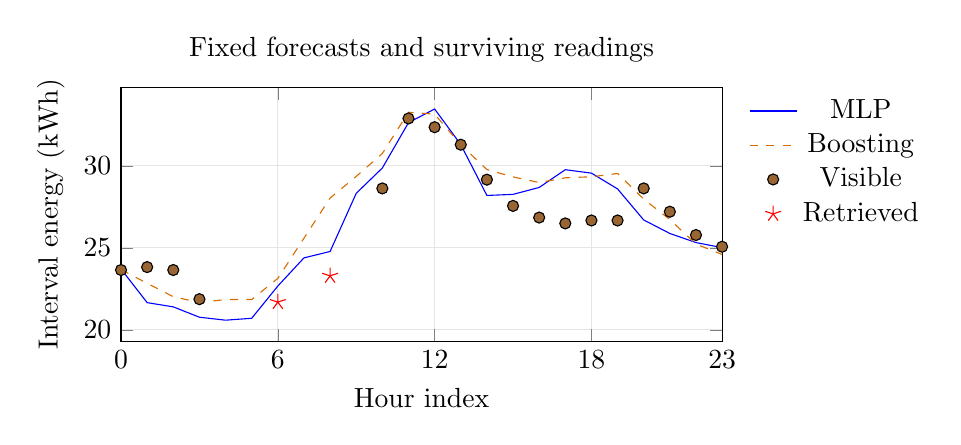
\begin{tikzpicture}
\begin{axis}[width=0.76\linewidth,height=4.8cm,tick label style={font=\normalsize},label style={font=\normalsize},legend style={font=\normalsize,draw=none},grid=major,grid style={gray!20},scaled ticks=false,xmin=0,xmax=23,xtick={0,6,12,18,23},xlabel={Hour index},ylabel={Interval energy (kWh)},legend pos=outer north east,title={Fixed forecasts and surviving readings}]
\addplot+[blue,mark=none] coordinates {(0,23.7089731) (1,21.65926053) (2,21.40056945) (3,20.76969428) (4,20.58918072) (5,20.7049956) (6,22.67158609) (7,24.38967792) (8,24.77970026) (9,28.32769632) (10,29.87362605) (11,32.63845034) (12,33.47187004) (13,31.30219642) (14,28.19734887) (15,28.26401218) (16,28.68569787) (17,29.76830032) (18,29.55914475) (19,28.59682085) (20,26.70253117) (21,25.87983072) (22,25.3235942) (23,25.0144397)};
\addlegendentry{MLP}
\addplot+[orange!85!black,mark=none,dashed] coordinates {(0,23.67335923) (1,22.83729057) (2,22.02153812) (3,21.666634) (4,21.84769547) (5,21.84769547) (6,23.13793853) (7,25.58930242) (8,28.04009073) (9,29.35798188) (10,30.76006346) (11,33.27016375) (12,33.15826742) (13,31.29274311) (14,29.77802672) (15,29.3296904) (16,28.98399795) (17,29.27340546) (18,29.33811927) (19,29.53693981) (20,27.97449045) (21,26.7313281) (22,25.23573177) (23,24.59836533)};
\addlegendentry{Boosting}
\addplot+[black,only marks,mark=*] coordinates {(0,23.64864865) (1,23.82645804) (2,23.64864865) (3,21.87055477) (10,28.62731152) (11,32.89473684) (12,32.36130868) (13,31.29445235) (14,29.16073969) (15,27.56045519) (16,26.84921764) (17,26.49359886) (18,26.67140825) (19,26.67140825) (20,28.62731152) (21,27.20483642) (22,25.78236131) (23,25.07112376)};
\addlegendentry{Visible}
\addplot+[red,only marks,mark=star,mark size=3pt] coordinates {(6,21.69274538) (8,23.29302987)};
\addlegendentry{Retrieved}
\end{axis}
\end{tikzpicture}

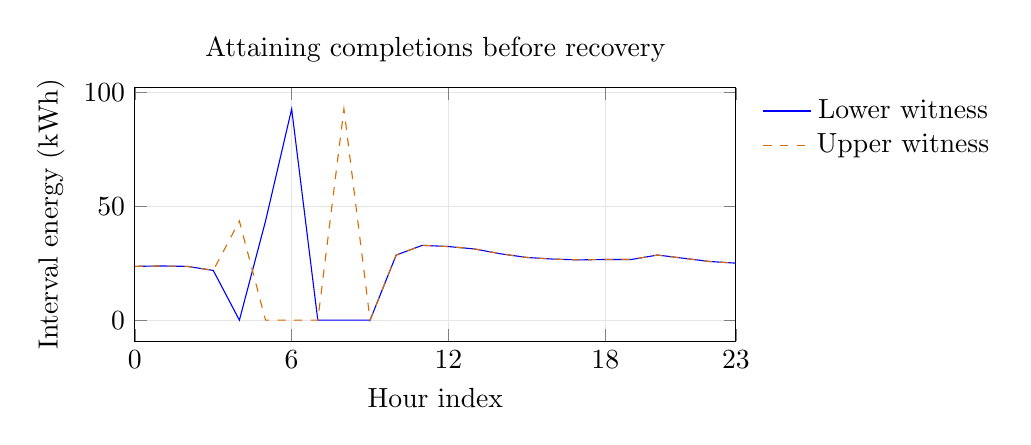
\begin{tikzpicture}
\begin{axis}[width=0.76\linewidth,height=4.8cm,tick label style={font=\normalsize},label style={font=\normalsize},legend style={font=\normalsize,draw=none},grid=major,grid style={gray!20},scaled ticks=false,xmin=0,xmax=23,xtick={0,6,12,18,23},xlabel={Hour index},ylabel={Interval energy (kWh)},legend pos=outer north east,title={Attaining completions before recovery}]
\addplot+[blue,mark=none] coordinates {(0,23.64864865) (1,23.82645804) (2,23.64864865) (3,21.87055477) (4,0) (5,43.56330014) (6,92.81650071) (7,0) (8,0) (9,0) (10,28.62731152) (11,32.89473684) (12,32.36130868) (13,31.29445235) (14,29.16073969) (15,27.56045519) (16,26.84921764) (17,26.49359886) (18,26.67140825) (19,26.67140825) (20,28.62731152) (21,27.20483642) (22,25.78236131) (23,25.07112376)};
\addlegendentry{Lower witness}
\addplot+[orange!85!black,mark=none,dashed] coordinates {(0,23.64864865) (1,23.82645804) (2,23.64864865) (3,21.87055477) (4,43.56330014) (5,0) (6,0) (7,0) (8,92.81650071) (9,0) (10,28.62731152) (11,32.89473684) (12,32.36130868) (13,31.29445235) (14,29.16073969) (15,27.56045519) (16,26.84921764) (17,26.49359886) (18,26.67140825) (19,26.67140825) (20,28.62731152) (21,27.20483642) (22,25.78236131) (23,25.07112376)};
\addlegendentry{Upper witness}
\end{axis}
\end{tikzpicture}

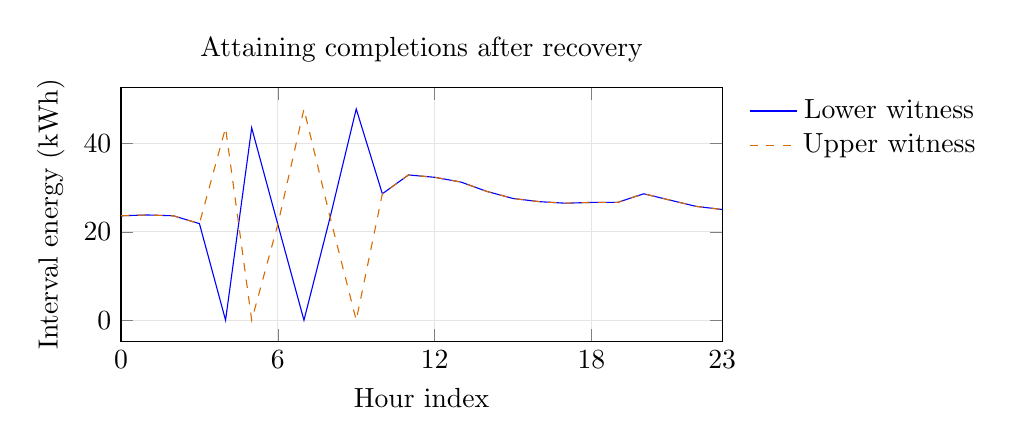
\begin{tikzpicture}
\begin{axis}[width=0.76\linewidth,height=4.8cm,tick label style={font=\normalsize},label style={font=\normalsize},legend style={font=\normalsize,draw=none},grid=major,grid style={gray!20},scaled ticks=false,xmin=0,xmax=23,xtick={0,6,12,18,23},xlabel={Hour index},ylabel={Interval energy (kWh)},legend pos=outer north east,title={Attaining completions after recovery}]
\addplot+[blue,mark=none] coordinates {(0,23.64864865) (1,23.82645804) (2,23.64864865) (3,21.87055477) (4,0) (5,43.56330014) (6,21.69274538) (7,0) (8,23.29302987) (9,47.83072546) (10,28.62731152) (11,32.89473684) (12,32.36130868) (13,31.29445235) (14,29.16073969) (15,27.56045519) (16,26.84921764) (17,26.49359886) (18,26.67140825) (19,26.67140825) (20,28.62731152) (21,27.20483642) (22,25.78236131) (23,25.07112376)};
\addlegendentry{Lower witness}
\addplot+[orange!85!black,mark=none,dashed] coordinates {(0,23.64864865) (1,23.82645804) (2,23.64864865) (3,21.87055477) (4,43.56330014) (5,0) (6,21.69274538) (7,47.83072546) (8,23.29302987) (9,0) (10,28.62731152) (11,32.89473684) (12,32.36130868) (13,31.29445235) (14,29.16073969) (15,27.56045519) (16,26.84921764) (17,26.49359886) (18,26.67140825) (19,26.67140825) (20,28.62731152) (21,27.20483642) (22,25.78236131) (23,25.07112376)};
\addlegendentry{Upper witness}
\end{axis}
\end{tikzpicture}
\caption{Frozen restricted-record daily evaluation; no saved-archive reconstruction. Worked historical audit, meter \texttt{MT\_002} on 2014-01-01. Lower and upper witnesses attain the bounds on MLP-minus-boosting MSE; they are measurement-compatible extremal completions, not predicted load profiles. The first chronologically unresolved eligible case was selected before inspecting the recovery outcome. Retrieved values come from the held-out reference trace. Full values and retained totals are in \texttt{study\_operator\_example.csv}.}
\label{fig:operator}\end{figure}

\FloatBarrier


\subsection{Restricted-record sensitivity}
The isolated daily-record experiment is a separate limited-input benchmark.
Appendices~\ref{app:restricted-daily} and~\ref{app:restricted-recovery}
retain its complete comparisons and budget grid. Its large recovery gains
must not be interpreted as gains after the saved archive has already been
used. The archive-consistent evidence above is the primary retrospective
application result.




\subsection{Attribution and the exact-versus-greedy distinction}
In the original restricted-record six-hour experiment, exact recovery exceeds
greedy certification by 1.15 percentage points on average across Portugal
meters. Exact alone certifies 785 dependent cases and greedy alone 119;
actual width is larger under exact recovery in 700 cases. Thus the worst-case
width optimum is not a pointwise certification optimum.
The preceding archive-consistent analysis isolates the much smaller
archive-aware allocator increment from free reconstruction and paid readings.
Appendix~\ref{app:greedy-detail} retains query counts, signed distributions
and descriptive bootstrap intervals.


\subsection{Total uncertainty and selective missingness}
Table~\ref{tab:sensitivity} retains every mask mechanism and total-error
setting for six missing targets and six-hour totals. Widening total
uncertainty enlarges the feasible set and cannot improve the mathematical
certificate. The contiguous, scattered, and highest-demand masks test
different locations of missing energy and forecast disagreement. The
highest-demand mask is an oracle stress condition, not a learned or
prospective outage predictor.
\begin{table}[htbp]
\centering\normalsize\setlength{\tabcolsep}{4pt}
\caption{Frozen restricted-record daily evaluation; no saved-archive reconstruction. Daily paired resolution (\%) with six missing targets and six-hour totals. High demand is an oracle stress mask. Every issued decision remained correct.}
\label{tab:sensitivity}
\begin{tabular}{llrrr}
\toprule
Source & Mask & Exact & $1\%$ & $5\%$\\
\midrule
Portugal & Contiguous & 18.8 & 18.1 & 15.8\\
Portugal & Scattered & 32.0 & 28.9 & 20.2\\
Portugal & High demand & 15.4 & 14.6 & 11.9\\
Household & Contiguous & 48.9 & 47.9 & 44.6\\
Household & Scattered & 67.8 & 65.2 & 57.0\\
Household & High demand & 32.5 & 31.6 & 27.3\\
Counters & Contiguous & 43.9 & 42.9 & 39.8\\
Counters & Scattered & 67.3 & 65.1 & 57.1\\
Counters & High demand & 35.8 & 34.7 & 30.3\\
\bottomrule
\end{tabular}
\end{table}

\FloatBarrier
\subsection{Numerical verification and execution cost}
The revised reference, integration, recovery, and malformed-input tests
passed. The study additionally passed 1,000
random study/reference cross-checks. Independent LP/QP audits and an
exhaustive adaptive-query oracle provide checks beyond the implementation's
own formulas. Their reports and source hashes accompany the manuscript.
The largest absolute LP discrepancy was $1.14\times10^{-13}$
across 1800 extrema; the corresponding
individual-error minimum discrepancy was $1.06\times10^{-9}$
across 600 constrained optimizations.
The adaptive oracle checked 5,952 finite small cases, including determined
last-coordinate queries and excess budgets, with exact agreement between
adaptive, exhaustive fixed-batch, and sorted-window optima.

On an Intel Core i7-8565U CPU with 15.75 GiB RAM, the revised main
pipeline took 809.8 s using two computation
threads and no GPU. Prepared-input timing used 30 feasible cases at each
length, five warmups, and three repetitions. The validated reference API
returned both extrema and witnesses in median 0.172 ms for
24 targets and 0.858 ms for 168 targets.
Two SciPy HiGHS calls on prepared matrices took
5.151 and
5.954 ms, respectively.
These measurements include solver-call overhead and exclude fitting and
file processing. They describe one host under uncontrolled concurrent
activity; no end-to-end forecasting speedup is inferred.

The additional two-query batch optimizer was timed on 30 prepared
24-target problems at each gap size, with five warmups and three repeats.
Its median latency was 0.057 ms for
six missing targets and 0.058 ms for
twelve. This measures query selection alone; input preparation, retrieval
from a real meter or archive, and recomputation of the bounds are excluded.
The experiment does not measure communication latency.

The separate interval-total batch solver was checked on 86
small synthetic instances by enumerating 1,247
query subsets and computing extrema using 3,458
HiGHS linear-program solves. It also passed 482
conditional-answer checks, 108
reductions to the exact-total implementation, and 25
invalid-input checks. The maximum recorded discrepancy was zero in these
constructed cases; this is finite numerical verification, not an
outward-rounded arithmetic guarantee. This extension was not used to
replace or pool the primary exact-total meter results, and its tests do
not measure field deployment benefits.
\FloatBarrier

\subsection{Replication and total-uncertainty sensitivity}
The frozen additional 30-consumer panel increases restricted-record
certification from 25.02\% to 64.11\% with exact two-query recovery;
archive-aware certification instead starts at 96.87\% and reaches 98.57\%.
The archive-aware exact-over-greedy increment is 0.061 percentage points
(Appendix~\ref{app:replication-results}). This supports repeatability within
the same dataset and calendar, not independent infrastructure validation.
With constructed $\pm5\%$ total bands on the original Portugal traces,
certification increases from 15.8\% to 46.3\% under restricted access and
from 96.5\% to 98.1\% with the saved archive. Appendix~\ref{app:interval-results}
retains every cohort, tolerance and policy result.


\subsection{Exact randomized recovery: robust gain and realized tradeoff}
\label{sec:random-results}
Of the 20,736 fixed comparisons, 1,074 retain positive width after free
archive information and total deductions. The finite-game solutions have
2,341 positive-probability batches. Independent reconstruction checks all
20,736 cases, all positive batches, 19,662 permitted direct target copies,
and all 1,074 compact-versus-finite-game optima. The largest objective
discrepancy, divided by $\max(1,\text{initial width})$, is
$1.34\times10^{-13}$. No issued support-batch certificate contradicts
the reference comparison. These dependent checks validate the calculation;
their count is not an independent statistical sample size.

Table~\ref{tab:random-results} separates the robust objective from realized
outcomes. Portugal's mean normalized worst expected width decreases from
29.595\% to 26.673\% of its initial width, a relative reduction of 9.88\%
against the exact deterministic optimum. Its normalized expected width at
the actual record increases from 20.154\% to 23.670\%, or 17.45\% relatively.
The household reductions and increases are 6.66\% and 11.05\%, respectively.
Certification decreases slightly in both cohorts. The robust objective
improves strictly in 663 positive-width cases; realized expected width
improves in 14, worsens in 649, and is unchanged in the remaining 411.
No query-count advantage is claimed: both exact policies use two readings
in these positive-width cases.



This adverse realized tradeoff is consistent with the objective: minimizing
the largest expected ambiguity over all compatible records does not
minimize width or maximize certification at the particular realized load
profile. Randomization is therefore a robust-design option, not an
empirically dominant default replacement for deterministic recovery.

The compact implementation agrees with exhaustive finite-game programs on
all 42 synthetic cases to within $1.78\times10^{-13}$ absolute objective
error. Constructed $(m,r)=(4,2),(6,2),(9,3),(12,2)$ instances attain factors
2, 3, 3, and 6, respectively. These are sharpness examples, not estimates
of typical field gains. Table~\ref{tab:compact-scale} demonstrates that the
implementation need not enumerate all batches. The larger instance has
more than 3.65 billion size-six subsets but only 3,221 LP variables.
The independent sampler audit also checks its induced mixture, rather than
only whether sampled batches have the correct size: the largest recovered
coefficient discrepancy is $1.78\times10^{-15}$. All floating-point
projection and normalization corrections are recorded in Online Resource~1.

\begin{table}[htbp]\centering\small
\caption{Fixed one-block scalability checks. The batch counts are combinatorial
counts, not enumerated runs. LP variable counts include the epigraph. These
two synthetic configurations establish feasibility at these sizes, not an
asymptotic runtime benchmark.}\label{tab:compact-scale}
\begin{tabular}{rrrr}\toprule
Coordinates $m$&Budget $B$&Size-$B$ batches&Compact LP variables\\\midrule
60 & 4 & 487,635 & 846 \\
120 & 6 & 3,652,745,460 & 3,221 \\
\bottomrule\end{tabular}\end{table}


\subsection{Secondary optimization does not remove the observed penalty}
\label{sec:tie-results}
All 2,148 secondary LPs complete. Neither the dominance refinement nor the
uniform-completion refinement changes the realized expected width in any
of the 1,074 positive-width cases beyond the declared $10^{-9}$ scaled
comparison tolerance. Neither strictly improves the secondary objective at
that tolerance. The largest normalized primary lower-bound gap is
$1.96\times10^{-12}$ and the largest dominance residual is
$5.75\times10^{-12}$. Portugal's normalized expected width remains
23.670\% for both refinements, versus 20.154\% for deterministic recovery;
certification remains 98.688\% versus 98.795\%. The household summaries
are likewise unchanged at the displayed precision. Independent replay checks
every refined distribution, secondary optimum, and case aggregation.
Thus the reported 17.45\% Portugal penalty persists under these specified
target-independent tie refinements. It is not evidence that every minimax
policy has that penalty, or that the percentage transfers to other records.
The exact counterexample in Section~\ref{sec:tie-selection} remains a useful
regression test even though this empirical panel shows no such improvement.

\subsection{Randomized recovery on additional consumers}
We subsequently froze the uniform-barycenter secondary rule and applied it to the existing 30-consumer Portugal replication: all 3,210 meter-days and all six model pairs (19,260 cases), without refitting. The information regime used the same six-hour contiguous mask, seed 1103, exact six-hour totals, saved persistence copies, exact-total closure, and budget $B=2$. Masked observations and measurement totals were first exported to a selection-only archive. A separate process optimized policies from these inputs, without opening the reference-target archive; the policies were hashed before realized-performance evaluation. This is a post-review audit of an existing held-out-consumer archive, not a prospective study or a new data source.

Of the 19,260 cases, 899 retained positive width after free reconstruction and closure; all were evaluated. Every positive-width case passed both the finite-game primal--dual checks and a comparison with the compact formulation, with maximum normalized objective discrepancy $6.94\times10^{-14}$. The independent arithmetic replay checked archive reconstruction, selected-batch interval containment, query budgets, and the saved primary dual bounds. All 3,958 positive-probability batches across the secondary policy and the original primary optimizer passed containment checks.

The adverse realized-performance result persisted. Consumer-macro worst-width fractions were 0.28112 for deterministic recovery and 0.25501 for the secondary randomized policy; realized-width fractions were 0.18497 and 0.21935, respectively. These fractions divide each consumer's summed posterior widths by its summed initial width, then average over consumers. All-case certification was 98.894\% versus 98.776\%, and positive-width-case certification was 76.318\% versus 73.798\%; these are consumer-macro averages of case-level certification probabilities. Mean paid queries were equal to the displayed precision: 0.09330 over all cases and 1.99885 in the positive-width stratum. Among the 899 positive-width cases, randomization strictly reduced worst width in 564; its realized width improved in 12, worsened in 553, and tied in 334 relative to deterministic recovery. The original primary optimizer gave the same aggregate results at the displayed precision. Thus the frozen secondary criterion did not remove the practical tradeoff on these additional consumers.

\subsection{Computational scaling of randomized recovery}

We froze 28 synthetic cases before optimization: the full factorial $G\in\{1,2,4\}$, $m\in\{6,12\}$, $B=\lfloor Gmf\rfloor$, $f\in\{1/4,1/2\}$, and two coefficient/total profiles, plus four single-block cases with $m\in\{24,48\}$ and $f=1/2$. The profiles were distinct coefficients with homogeneous totals, and threefold coefficient ties with geometric coefficient scales and heterogeneous totals. Thus ties and heterogeneity vary jointly; the comparison does not isolate either effect. The manifest fixes every coefficient, total, seed, budget, and exhaustive-solver eligibility decision.

Each method/case ran once in a fresh subprocess on an Intel Core i7-8565U (four physical cores, 16.9 GB RAM), Windows 11, Python 3.12.14, NumPy 2.5.3, and SciPy 1.18.1. HiGHS and numerical-library thread limits were one. Method time includes LP construction, solution, and policy compilation after imports; separately measured diagnostic overhead is removed. Peak working set is the worker-reported whole-process peak, including interpreter and imports. The wall limit was 20 s. A parent memory watchdog used a 1 GiB threshold, but the Windows environment launcher can make that watchdog observe the redirector; therefore it is not a verified worker allocation cap. Every worker-reported peak was below 169 MiB. Runs were sequential on a shared host, without timing repetitions.

All 28 compact runs returned an optimal LP and passed 560 seeded exact-budget/sample-identity checks. Maximum normalized primal violation, stationarity residual, and primal--dual gap were $3.78\times10^{-15}$, $5.22\times10^{-15}$, and $5.78\times10^{-16}$, respectively; the recorded dual sign violation was zero. Exhaustive finite-game comparison was prescribed only for at most 25,000 admissible batches and at most 100,000 prefilter Cartesian-product candidates. All 12 eligible comparisons ran, with maximum objective discrepancy $1.27\times10^{-15}$ after division by $\max(1,W_0)$; the other 16 were retained as predetermined skips. There were no timeouts, solver errors, or memory terminations.
Table~\ref{tab:compact-scaling-audit} reports both profiles at every dimension/budget setting. Its ranges span two different instances, not repeated-run uncertainty. Full per-case objectives, sparse dimensions/nonzeros, timings, memory, and numerical diagnostics are archived. These bounded measurements establish operability at the sampled sizes; they do not establish runtime dominance or empirical asymptotic complexity, and the residual checks are floating-point evidence rather than exact certificates.


% Standalone integration fragment, based on panel_summary.json and immutable
% recorded source/decode snapshots. Does not claim natural hidden-label truth.
\subsection{Natural precipitation accumulations: a zero-query audit}
\label{sec:noaa-natural}
The aggregate-only information structure also occurs without deliberately
removing fine-resolution labels. NOAA's COOP Hourly Precipitation Data retain
legacy records in which an accumulation total is reported but its distribution
over the intervening hours is unavailable \cite{noaa_hpd_v2,noaa_hpd_format}.
This supports a limited retrospective verification task: determine whether two
fixed forecasts can be ordered for every temporal allocation consistent with
the archived total. It does not establish that historical hourly readings can
be recovered, or assign a cost to recovering them.

We fixed a small source-based panel before inspecting forecast comparisons.
A lexical screen of the first three CONUS station files found nine simple
one-day accumulation records after 2000 at Alberta, Alabama
(USC00010140; $32.2322^{\circ}$N, $87.4104^{\circ}$W). All nine occur in December
2008 or June 2009 and are retained. We also retain every eligible complete day
in those two months. Of 61 calendar dates, 52 are included: nine accumulation
days and 43 complete days. Seven dates have no hourly row, and two contain
multi-day accumulations outside this fixed one-day design. Selection is
purposive and does not estimate the prevalence of useful coarse records.

On each natural case, the hourly record has a beginning flag at 00:00,
interior accumulation flags, and an ending flag with the total at 23:00.
The current CSV definition assigns these fields to $[00{:}00,01{:}00)$ and
$[23{:}00,24{:}00)$ local standard time, respectively. Thus the constraint
covers the full 24-hour recorded day. Values in hundredths of an inch are
converted to millimetres by multiplication by $0.254$. We use the original
accumulation total, never the computed \texttt{DlySum} field as an independent
measurement. The station inventory specifies UTC$-6$ in both months.

The permitted public-source audit includes the parallel 15-minute station
file and the digital raw-data files for both months. For the six December
cases, the parallel file supplies three initial zero quarter-hours followed
by the same unresolved accumulation and matching total. The three June
event dates are absent. No selected station record is present in either
monthly digital raw file. These findings are preserved with source-row
pointers and hashes. Initial zero quarter-hours do not identify any complete
three-hour target: every three-hour bin still contains unconstrained
nonnegative periods, so projecting the checked information onto the eight
bins leaves $y\geq0$ and $\sum_i y_i=T$. Several legacy download endpoints
returned HTTP 404; the conclusion concerns the documented files checked,
not a proof that no other archive exists.

We compare the GEFSv12 control member with the fixed arithmetic mean of its
five daily members, with no fitting or member selection
\cite{guan2022gefs,noaa_gefs_archive}. These are retrospective numerical
weather forecasts, not forecasts issued in 2008--2009 or an ML-performance
benchmark. The nearest $0.25^{\circ}$ grid point is 8.6565\,km from the station.
The nominal cycle is 00:00 UTC; Phase 2 integration actually starts at 03:00
UTC following the replay analysis. Guan et al.'s documented corrections
concern the initial 00:00--03:00 and 00:00--06:00 accumulated fields. We use
valid windows 06:00--06:00 the following day, checked against GRIB validity
metadata, corresponding to eight local three-hour bins. Nested three- and
six-hour precipitation fields are differenced. There were 28 negative
differences, between $-0.05$ and $-0.01$\,mm,
across 27 of 260 member-days. Each discrepancy passed the recorded packing
resolution bound; this establishes consistency with differential quantization,
not its exclusive causal explanation. Our specified nonnegative preprocessing caps the first
three-hour amount at its six-hour total and uses the residual for the second,
preserving every decoded six-hour total. All raw differences and the complete
raw-versus-processed endpoint sensitivity are retained.

Let $a$ denote the processed control and $b$ the processed ensemble mean.
For the daily mean squared-error contrast $\Delta=L(a)-L(b)$, the direct
paired bounds are compared with subtraction of separately sharp individual
MSE bounds using exactly the same information. Table~\ref{tab:noaa-natural}
reports all nine natural cases. Two days certify lower ensemble-mean MSE;
the separate individual bounds certify neither. One day is an exact forecast
tie and six permit both orderings. Uniform allocation gives point orderings
on all eight non-tie days, but six of those orderings are not implied by the
observed information. There is no fine-resolution truth with which to label
those point decisions correct or incorrect.

\begin{table}[t]
\centering
\caption{All natural accumulation cases. Bounds are for control minus
ensemble-mean MSE over eight three-hour bins, in $\mathrm{mm}^2$.
Positive intervals certify the ensemble mean.}
\label{tab:noaa-natural}
\begin{tabular}{lrrrl}
\hline
Date & Total (mm) & Lower & Upper & Conclusion\\
\hline
2008-12-05 & 12.700 & 0.00000 & 0.00000 & exact tie\\
2008-12-10 & 12.700 & 7.18081 & 25.37356 & ensemble\\
2008-12-11 & 33.020 & $-24.65680$ & 26.47467 & unresolved\\
2008-12-17 & 5.080 & $-0.48739$ & 0.43971 & unresolved\\
2008-12-28 & 5.080 & $-1.01836$ & 0.37356 & unresolved\\
2008-12-29 & 5.080 & $-0.04186$ & 0.03942 & unresolved\\
2009-06-05 & 7.874 & $-1.15768$ & 1.48011 & unresolved\\
2009-06-14 & 1.524 & 0.64919 & 1.47063 & ensemble\\
2009-06-24 & 9.652 & $-0.00005$ & 0.04821 & unresolved\\
\hline
\end{tabular}
\end{table}

The conclusions on all nine natural days are unchanged using raw signed
increments; preprocessing changes two dry-control conclusions to ties.
All 43 complete controls have zero recorded precipitation, predominantly
archive-assigned zero flags. Their feasible sets are singleton zero vectors,
so they test only this degenerate case and do not validate nonzero natural
endpoints against hidden truth. Combining their observed loss contrasts with
the nine natural intervals yields the 52-day interval
$[-0.250924,1.195845]\,\mathrm{mm}^2$, which does not order the forecasts.
We also fixed a supplementary $\pm2.54$\,mm total perturbation before inspecting
paired outcomes, motivated by NOAA's nominal $0.1$-inch gauge accuracy.
With $T\in[\max(0,T_0-2.54),T_0+2.54]$, only the 2008-12-10 strict certificate
remains. This is a source-inspired sensitivity, not a validated error bound
for the legacy totals or a confidence statement about physical rainfall.

This panel supplies a concrete natural use of zero-query partial-label
evaluation: some forecast comparisons are identifiable even when their
individual scores are not. Its scope is limited by the nine selected events,
recording and measurement uncertainty, and grid-point versus gauge
representativeness. It provides neither evidence of retrieval savings nor
a general ranking of the forecast systems. The lightweight archive contains
source excerpts, every decoded-message record and provenance pointer, both
forecast variants, and an offline executable reconstruction; fresh GRIB
decoding and full-source checks are distinguished from excerpt arithmetic.


\FloatBarrier
\section*{Supplementary Materials}
The present decision-acquisition revision is reproduced with
\texttt{python} \path{work/reproduce_decision_revision.py}. Its default route
checks the new source records, independently verifies confirmation trajectories
and exhaustive hindsight subsets, and rebuilds the present manuscript.
The \texttt{--development} option also checks the complete original validation
selection grid; \texttt{--legacy} adds the earlier external replay.
The \texttt{--refit} option runs new model fitting and confirmation in an
isolated stage, and \texttt{--small} runs mathematical fixtures. Replaying
saved forecasts does not constitute a fresh fit or external investigator
replication. The release pins every composition input and preserves earlier
negative outcomes and protocol amendments.
The independent randomized check verifies finite-game objectives and mixture
moments and support; it does not replay the compact sampler's exact random
draw. The complete sampler is supplied, and the fresh-fit route reruns its
acquisition.

The later query-eligibility review supplies an exact-rational
zero-coefficient fixture, calls to every production policy and the actual
hindsight driver, a complete audit of the earlier saved batches, and
synthetic batch-feasibility checks. Run
\texttt{python} \path{work/eligibility_review_20261011/check_review.py}.
These checks clarify eligibility and accounting; they do not refit models
or replace an empirical result. The associated diagnostic scripts explain
the small learned-policy gain from the already evaluated confirmation
traces and are explicitly retrospective.


The entry point for the preceding external revision is
\texttt{python} \path{work/reproduce_external_revision.py}. It checks the bundled
literal LCL source subset, independently replays all validation and test
trajectories and summaries, and reconstructs its earlier manuscript in an isolated
workspace. The \texttt{--small} route runs synthetic checks without reading
the large data. The \texttt{--refit} route reruns all external model fits and
acquisition from bundled hourly references; \texttt{--raw}, with the pinned
official archive and extracted CSV paths, first reconstructs those references
from the complete source. The documentation records commands, source hashes,
measured runtimes and the scope of each check. Saved-trajectory replay does
not imply a fresh fitting run. The original completed 60-model external
fitting execution is separately documented, including an earlier input-date
serialization failure and its unchanged-design correction. No test outcomes
were produced by that failed execution.

The first independent trajectory replay also detected aliasing in saved
intermediate observation snapshots. The logging assignment now copies its
array. The affected snapshots were reconstructed from their saved prior
states, recorded batch answers and totals; query choices, bounds, costs,
decisions and numerical summaries were unchanged. Original compressed
traces, execution metadata and evaluator source are retained. The independent
checker requires each original discrepancy to equal exactly the next
batch's recorded reveals and verifies the corrected state separately.
This disclosed logging repair is not a new policy run.

The supplement contains the selected literal LCL rows with attribution,
all considered household quality counts, model inputs, every issued forecast,
reference targets, archive source traces, acquisition sequences and per-case
and aggregate results. The full 8.54~GB raw CSV and extraction tool are
obtained separately using the documented official URL. Earlier historical
reproduction routes remain included with their original evidence and
redistribution boundaries. A release manifest distinguishes newly executed
external checks from byte-identical historical evidence carried forward.

\textbf{Online Resource 1: Reproducibility package.}
The accompanying \path{research_supplement.zip} contains implementations,
source-download and reproduction scripts, dated protocols, aggregate
results, frozen fitted-model forecasts, validation reports, and the
manuscript reconstruction scripts.

\section*{Statements and Declarations}
\subsection*{Data and Code Availability}
The source datasets are publicly identified in References
\cite{uci,portugal,blem,lcl}. Reproduction code, the documented protocol and its
dated amendments, complete scenario summaries, and
validation results accompany this manuscript as supplementary materials.
The supplement identifies exact source versions and checksums and recreates
the hourly targets from the original sources. The original fitting pipeline
is supplied separately from the no-refit evaluation reproduction.
\texttt{frozen\_forecasts.csv} supplies saved fitted-model forecasts for all
34 series, target timestamps, and simulated issue-time cutoffs; it also
includes persistence for the two UCI sources. BLEM persistence is omitted
because it directly copies earlier raw readings and can be regenerated.
For exact reproduction, \texttt{review\_frozen\_forecasts.csv} preserves
the original fitted-forecast text and the UCI targets, with only BLEM
targets and persistence omitted. Combining this lossless export with the
pinned raw targets restores all 89,496 original evaluation rows to the
original byte-level SHA-256 checksum without refitting. That reconstruction
has been executed; the supplied \texttt{--raw} mode reruns the corrected
analyses from these restored records. The default
\texttt{work/reproduce\_review\_revision.py} command independently checks
distributed UCI period traces and interval aggregates and rebuilds the
corresponding historical manuscript. The decision-revision entry point above rebuilds the present manuscript. Its BLEM checks reconcile aggregates; detailed BLEM case
reconstruction requires the full local records or raw mode. Full period
traces, archive-aware case endpoints and old per-day recovery cases that
could reveal omitted BLEM readings are replaced by UCI-only public exports
and omission manifests. Full local and raw-mode period checks cover all
34 series. The default mode does not claim an independent forecast refit
or a raw-data rerun.
The separate UCI-only new-consumer replication supplies its hourly targets
and all four forecasts under the source's CC BY 4.0 terms, with attribution
and preprocessing documented in the supplement.
The full
per-hour prediction/target archive is retained for the local analysis but
omitted from the submission supplement because a separate redistribution
license for the BLEM readings was not verified. Its checksum is recorded
so regenerated files can be checked. No public
repository publication is claimed beyond the cited original data sources.


The additional randomized-recovery materials include the compact optimizer,
an executable hard-budget sampler, complete finite-game primal/dual traces,
all positive query batches, an independent reconstruction of every public
energy case, and sharpness/scalability fixtures. The NOAA materials include
the selected observation records, decoded gridpoint predictions and message
provenance, the fixed source-selection protocol, all nine natural cases,
all 43 dry controls, failed-run diagnostics and the declared preprocessing
and tolerance sensitivities. Source URLs and content hashes identify the
downloaded records; the supplement does not include the large GRIB cache.
The naturally missing subdaily targets are not available as reference truth.

\subsection*{Research Transparency}
This study reanalyzes public meter and precipitation records and does not recruit participants
or collect new measurements. Artificial outages, constructed totals,
recorded counter increments, and assumed total-error ranges are distinguished
in the methods. All reported numerical results were calculated by the
accompanying code.

\subsection*{Funding and Competing Interests}
\textbf{Funding.} This research received no external funding.

\textbf{Competing interests.} The author declares no conflicts of interest.

\subsection*{Generative-AI Disclosure}
OpenAI Codex (OpenAI; accessed October 2026) assisted with literature
searches, mathematical review, programming, experimental execution, and
manuscript drafting. This assistance is distinct from the trained MLP and
boosted-tree forecasting models evaluated in the study.

\FloatBarrier
\begin{thebibliography}{99}

\bibitem{azuremonitor} Microsoft, ``Monitor the performance of models deployed
to production,'' Azure Machine Learning documentation, updated 11 February
2026. \url{https://learn.microsoft.com/en-us/azure/machine-learning/how-to-monitor-model-performance?view=azureml-api-2}.

\bibitem{awsmonitor} Amazon Web Services, ``Model Monitor FAQs,'' Amazon
SageMaker AI Developer Guide, accessed 9 October 2026.
\url{https://docs.aws.amazon.com/sagemaker/latest/dg/model-monitor-faqs.html}.

\bibitem{canada} Measurement Canada, ``GEN-31---Policy on multirate register
metering,'' sec.~5.7, revised 2010.
\url{https://ised-isde.canada.ca/site/measurement-canada/en/laws-and-requirements/gen-31-policy-multirate-register-metering}.

\bibitem{norpen} A. Vavouris, F. Guasselli, L. Stankovic, V. Stankovic,
K. Gram-Hanssen, and S. Didierjean, ``Descriptor: A Norwegian positive
energy neighborhood dataset of electrical measurements and interviews on
energy practices (NorPEN),'' \emph{IEEE Data Descriptions}, vol.~1, 2024.
\url{https://doi.org/10.1109/IEEEDATA.2024.3483154}.

\bibitem{elexon} Elexon, ``BSCP702: Advanced Data Service,'' version 2.0,
effective 6 November 2025, secs.~4.2.7A--B, 4.2.16--17, and 4.2.21.
\url{https://bscdocs.elexon.co.uk/bsc-module/bsc-procedures/bscp702-advanced-data-service}.

\bibitem{aemo} Australian Energy Market Operator,
``Metrology procedure: Part B---Metering data validation, substitution
and estimation,'' version~8.13, effective June~9, 2026,
secs.~2.4--2.5 and 3.2.
\url{https://www.aemo.com.au/-/media/files/electricity/nem/retail_and_metering/market_settlement_and_transfer_solutions/2026/metrology-procedure-part-b-v813-clean.pdf}.

\bibitem{manski} C. F. Manski, ``Partial identification with missing data:
Concepts and findings,'' \emph{International Journal of Approximate
Reasoning}, vol.~39, pp.~151--165, 2005.
\url{https://doi.org/10.1016/j.ijar.2004.10.006}.

\bibitem{polo} F. Maia Polo, S. Maity, M. Yurochkin, M. Banerjee, and
Y. Sun, ``Weak supervision performance evaluation via partial
identification,'' \emph{Advances in Neural Information Processing
Systems}, vol.~37, 2024. \url{https://arxiv.org/abs/2312.04601}.

\bibitem{bessac} J. Bessac and P. Naveau, ``Forecast score distributions
with imperfect observations,'' \emph{Advances in Statistical Climatology,
Meteorology and Oceanography}, vol.~7, pp.~53--71, 2021.
\url{https://doi.org/10.5194/ascmo-7-53-2021}.

\bibitem{patton} A. J. Patton, ``Volatility forecast comparison using
imperfect volatility proxies,'' \emph{Journal of Econometrics}, vol.~160,
no.~1, pp.~246--256, 2011. \url{https://doi.org/10.1016/j.jeconom.2010.03.034}.

\bibitem{cpi} M. Weber, M. Turowski, H. K. \c{C}akmak, R. Mikut,
U. K\"uhnapfel, and V. Hagenmeyer, ``Data-driven copy-paste imputation
for energy time series,'' \emph{IEEE Transactions on Smart Grid},
vol.~12, no.~6, pp.~5409--5419, 2021.
\url{https://doi.org/10.1109/TSG.2021.3101831}.

\bibitem{hu} S. Hu, H. Dai, F. Meng, L. Aslett, M. Pollock, and
G. O. Roberts, ``Statistical disaggregation---A Monte Carlo approach
for imputation under constraints,'' \emph{Scandinavian Journal of
Statistics}, vol.~52, no.~3, pp.~1376--1421, 2025.
\url{https://doi.org/10.1111/sjos.12790}.

\bibitem{heat} M. Schaffer, T. Tvedebrink, and A. Marszal-Pomianowska,
``Three years of hourly data from 3021 smart heat meters installed in
Danish residential buildings,'' \emph{Scientific Data}, vol.~9,
art.~420, 2022. \url{https://doi.org/10.1038/s41597-022-01502-3}.

\bibitem{sawade} C. Sawade, N. Landwehr, and T. Scheffer,
``Active comparison of prediction models,''
\emph{Advances in Neural Information Processing Systems}, vol.~25, 2012.
\url{https://proceedings.neurips.cc/paper_files/paper/2012/file/92fb0c6d1758261f10d052e6e2c1123c-Paper.pdf}.

\bibitem{hara} S. Hara, M. Matsuura, J. Honda, and S. Ito,
``Active model selection: A variance minimization approach,''
\emph{Machine Learning}, vol.~113, pp.~8327--8345, 2024.
\url{https://doi.org/10.1007/s10994-024-06603-1}.

\bibitem{javdani2014} S. Javdani, Y. Chen, A. Karbasi, A. Krause,
D. Bagnell, and S. Srinivasa, ``Near Optimal Bayesian Active Learning for
Decision Making,'' in \emph{Proceedings of the Seventeenth International
Conference on Artificial Intelligence and Statistics}, \emph{Proceedings
of Machine Learning Research}, vol.~33, pp.~430--438, 2014.
\url{https://proceedings.mlr.press/v33/javdani14.html}.

\bibitem{active} J. Kossen, S. Farquhar, Y. Gal, and
T. Rainforth, ``Active testing: Sample-efficient model evaluation,''
\emph{Proceedings of Machine Learning Research}, vol.~139,
pp.~5753--5763, 2021.
\url{https://proceedings.mlr.press/v139/kossen21a.html}.

\bibitem{okanovic2025} P. Okanovic, A. Kirsch, J. Kasper, T. Hoefler,
A. Krause, and N. M. G\"urel, ``All models are wrong, some are useful:
Model Selection with Limited Labels,'' in \emph{Proceedings of the 28th
International Conference on Artificial Intelligence and Statistics},
\emph{Proceedings of Machine Learning Research}, vol.~258, pp.~2035--2043,
2025. \url{https://proceedings.mlr.press/v258/okanovic25a.html}.

\bibitem{ddid} P. Vayanos, A. Georghiou, and H. Yu,
``Robust optimization with decision-dependent information discovery,''
\emph{Management Science}, vol.~72, no.~2, pp.~1509--1528, 2026
(published online June 2025).
\url{https://doi.org/10.1287/mnsc.2021.00160}.

\bibitem{chen2026} X. Chen, M. Goerigk, and M. Poss, ``The robust selection
problem with information discovery,'' \emph{Discrete Applied Mathematics},
vol.~382, pp.~277--292, 2026. \url{https://doi.org/10.1016/j.dam.2025.12.012}.

\bibitem{kawase2024}
Y.~Kawase and H.~Sumita, ``Randomized strategies for robust combinatorial
optimization with approximate separation,'' \emph{Algorithmica}, vol.~86,
pp.~566--584, 2024. \url{https://doi.org/10.1007/s00453-023-01175-3}.

\bibitem{aggarwal} A. Aggarwal, H. Imai, N. Katoh, and S. Suri, ``Finding
$k$ points with minimum diameter and related problems,'' \emph{Journal of
Algorithms}, vol.~12, no.~1, pp.~38--56, 1991,
\url{https://doi.org/10.1016/0196-6774(91)90022-Q}.

\bibitem{martin1990} R. K. Martin, R. L. Rardin, and B. A. Campbell,
``Polyhedral Characterization of Discrete Dynamic Programming,''
\emph{Operations Research}, vol.~38, no.~1, pp.~127--138, 1990.
\url{https://doi.org/10.1287/opre.38.1.127}.

\bibitem{iancu2014} D. A. Iancu and N. Trichakis, ``Pareto efficiency in robust
optimization,'' \emph{Management Science}, vol.~60, no.~1, pp.~130--147, 2014.
\url{https://doi.org/10.1287/mnsc.2013.1753}.

% Verified against the official Springer article/chapter pages, 10 October 2026.
% Kawase--Sumita appeared online in 2023; its journal volume year is 2024.

\bibitem{osipenko} K. Yu. Osipenko,
``Generalized adaptive versus nonadaptive recovery from noisy information,''
\emph{Journal of Complexity}, vol.~53, pp.~162--172, 2019.
\url{https://doi.org/10.1016/j.jco.2018.12.001}.

\bibitem{mastin2015}
A.~Mastin, P.~Jaillet, and S.~Chin, ``Randomized minmax regret for
combinatorial optimization under uncertainty,'' in \emph{Algorithms and
Computation (ISAAC 2015)}, Lecture Notes in Computer Science, vol.~9472,
Springer, 2015, pp.~491--501.
\url{https://doi.org/10.1007/978-3-662-48971-0_42}.

% Primary full texts / metadata:
% https://link.springer.com/article/10.1007/s00453-023-01175-3
% https://link.springer.com/chapter/10.1007/978-3-662-48971-0_42
% Author-hosted Mastin et al. accepted text:
% https://www.mit.edu/~jaillet/general/rand_mmr_final.pdf

\bibitem{lcl} UK Power Networks, ``SmartMeter Energy Consumption Data in
London Households,'' London Datastore, dataset, accessed 11 October 2026.
Official full archive, CC BY 4.0.
\url{https://data.london.gov.uk/dataset/smartmeter-energy-consumption-data-in-london-households-vqm0d}.

\bibitem{refitraw} D. Murray, L. Stankovic, and V. Stankovic,
``REFIT: Electrical Load Measurements,'' University of Strathclyde, dataset,
2015. Raw release \texttt{REFIT\_RAW\_081116.7z}, CC BY 4.0.
\url{https://doi.org/10.15129/31da3ece-f902-4e95-a093-e0a9536983c4}.

\bibitem{botacin2025} M. Botacin and H. Gomes, ``Towards more realistic
evaluations: The impact of label delays in malware detection pipelines,''
\emph{Computers \& Security}, vol.~148, art.~104122, 2025.
\url{https://doi.org/10.1016/j.cose.2024.104122}.

\bibitem{savage} L. J. Savage, ``The theory of statistical decision,''
\emph{Journal of the American Statistical Association}, vol.~46,
pp.~55--67, 1951. \url{https://doi.org/10.1080/01621459.1951.10500768}.

\bibitem{manskiregret} C. F. Manski, ``Minimax-regret treatment choice
with missing outcome data,'' \emph{Journal of Econometrics}, vol.~139,
pp.~105--115, 2007. \url{https://doi.org/10.1016/j.jeconom.2006.06.006}.

\bibitem{sensorsel} Y. Wang, M. Sznaier, and F. Dabbene,
``A convex optimization approach to worst-case optimal sensor selection,''
in \emph{Proceedings of the 52nd IEEE Conference on Decision and Control},
pp.~6353--6358, 2013.
\url{https://robustsystems.coe.neu.edu/sites/robustsystems.coe.neu.edu/files/systems/papers/Yin_CDC13.pdf}.

\bibitem{portugal} A. Trindade, ``ElectricityLoadDiagrams20112014,''
UCI Machine Learning Repository, dataset, 2015.
\url{https://doi.org/10.24432/C58C86}.

\bibitem{uci} G. Hebrail and A. Berard, ``Individual household electric
power consumption,'' UCI Machine Learning Repository, dataset, 2006.
\url{https://doi.org/10.24432/C58K54}.

\bibitem{blem} M. Kostmann and W. K. H\"ardle,
``Forecasting in blockchain-based local energy markets,''
\emph{Energies}, vol.~12, art.~2718, 2019.
\url{https://doi.org/10.3390/en12142718}.
Source data: \url{https://github.com/QuantLet/BLEM}.

\bibitem{noaa_hpd_v2}
D.~Wuertz, J.~Lawrimore, and B.~Korzeniewski,
``NOAA Cooperative Observer Program (COOP) Precipitation Data---Hourly,
Version 2,'' NOAA National Centers for Environmental Information, 2018.
Station USC00010140, December 2008 and June 2009; accessed 10 October 2026.
\url{https://doi.org/10.25921/p7j8-2170}.

\bibitem{noaa_hpd_format}
NOAA National Centers for Environmental Information,
``README file for COOP Hourly Precipitation Data, CSV format,''
and parallel 15-minute archive format documentation, accessed 10 October 2026.
\url{https://www.ncei.noaa.gov/data/coop-hourly-precipitation/v2/doc/readme.csv.txt};
\url{https://www.ncei.noaa.gov/pub/data/hpd/auto/v2/beta/15min/readme.15min.txt}.

\bibitem{guan2022gefs}
H.~Guan et al., ``GEFSv12 Reforecast Dataset for Supporting Subseasonal
and Hydrometeorological Applications,'' \emph{Monthly Weather Review},
vol.~150, pp.~647--665, 2022.
\url{https://doi.org/10.1175/MWR-D-21-0245.1}.

\bibitem{noaa_gefs_archive}
NOAA, ``GEFSv12 reforecast data: archive description,'' accessed 10 October 2026.
\url{https://noaa-gefs-retrospective.s3.amazonaws.com/Description_of_reforecast_data.pdf}.
\end{thebibliography}
\end{document}
